\chapter{Integration and Installation}
\label{ch:int-inst}

\fixme{Note: the R/O link for the CDR chapter on ND-LAr is https://www.overleaf.com/read/djjrpnnxzbfp}
\fixme{Anne is putting in info from google sheet}
%%%%%%%%%%%%%%%%%%%%%%%%%%%%%%%%
\section{Introduction and Near Detector Facility Layout} 
\label{sec:int-inst-intro}

\subsection{Near Detector Cavern Layout}
\label{sec:chap-id:introduction:layout}

The DUNE ND cavern, which accommodates the DUNE ND with its component subdetectors ND-LAr, ND-GAr, and SAND,  will be located on the western-most boundary of Fermi National Laboratory.   Figure~\ref{fig:nd_hall_location} shows a birds-eye view of the future LBNF/DUNE construction site with the FNAL main injector, the target hall, decay pipe, muon absorber, and the Near Detector hall locations indicated. A cross-sectional view of the near site beamline is shown in Figure~\ref{fig:near_site_xsec}. As illustrated the near detector hall will be located about \SI{570}{\m} from the proton beam target at an underground depth of approximately \SI{60}{\m}. This is the furthest possible separation from the target hall within the FNAL property boundary.

\begin{dunefigure}[Top view of the future LBNF/DUNE construction site]{fig:nd_hall_location}
{Birds-eye view of the future LBNF/DUNE construction site. The Near Detector cavern will be located at the west-most boundary of Fermi National Lab.}
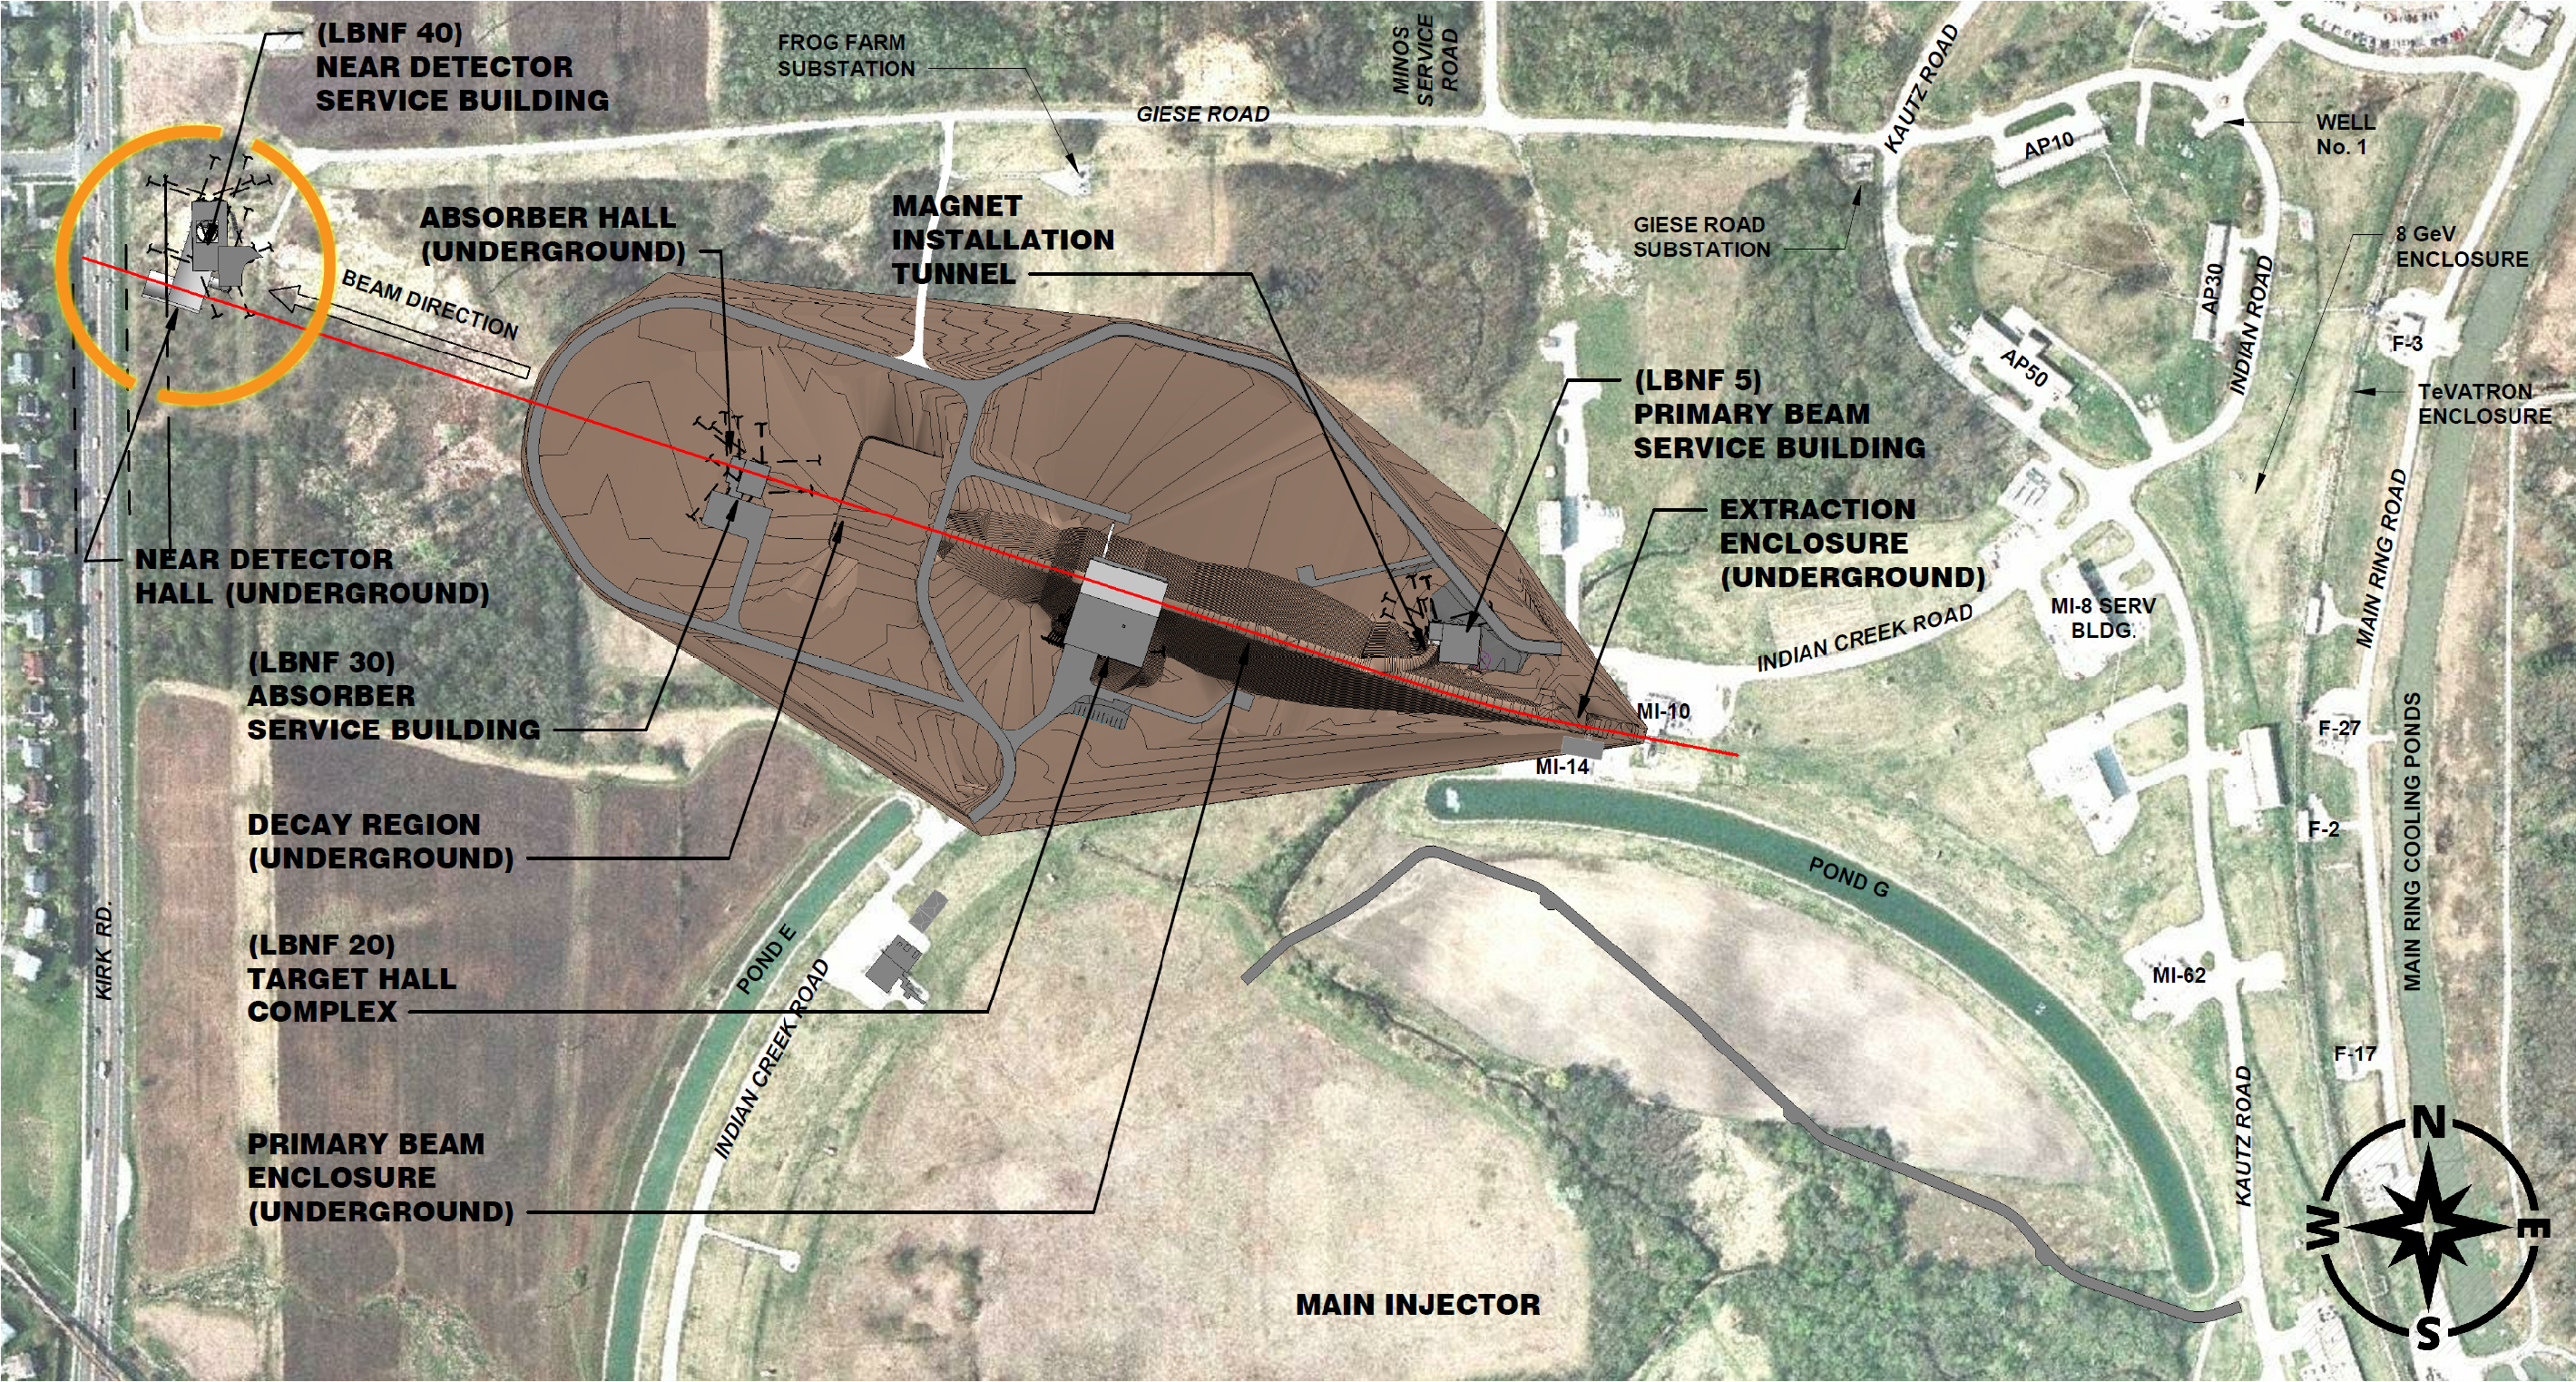
\includegraphics[width=0.8\textwidth]{graphics/i-and-i/nd_hall_location}
\end{dunefigure}


\begin{dunefigure}[Cross-sectional view of the near site beamline]{fig:near_site_xsec}
{A cross-sectional view of the near site neutrino beamline. The near detector hall will be located about \SI{570}{\m} from the proton beam target at an underground depth of approximately \SI{60}{\m}.}
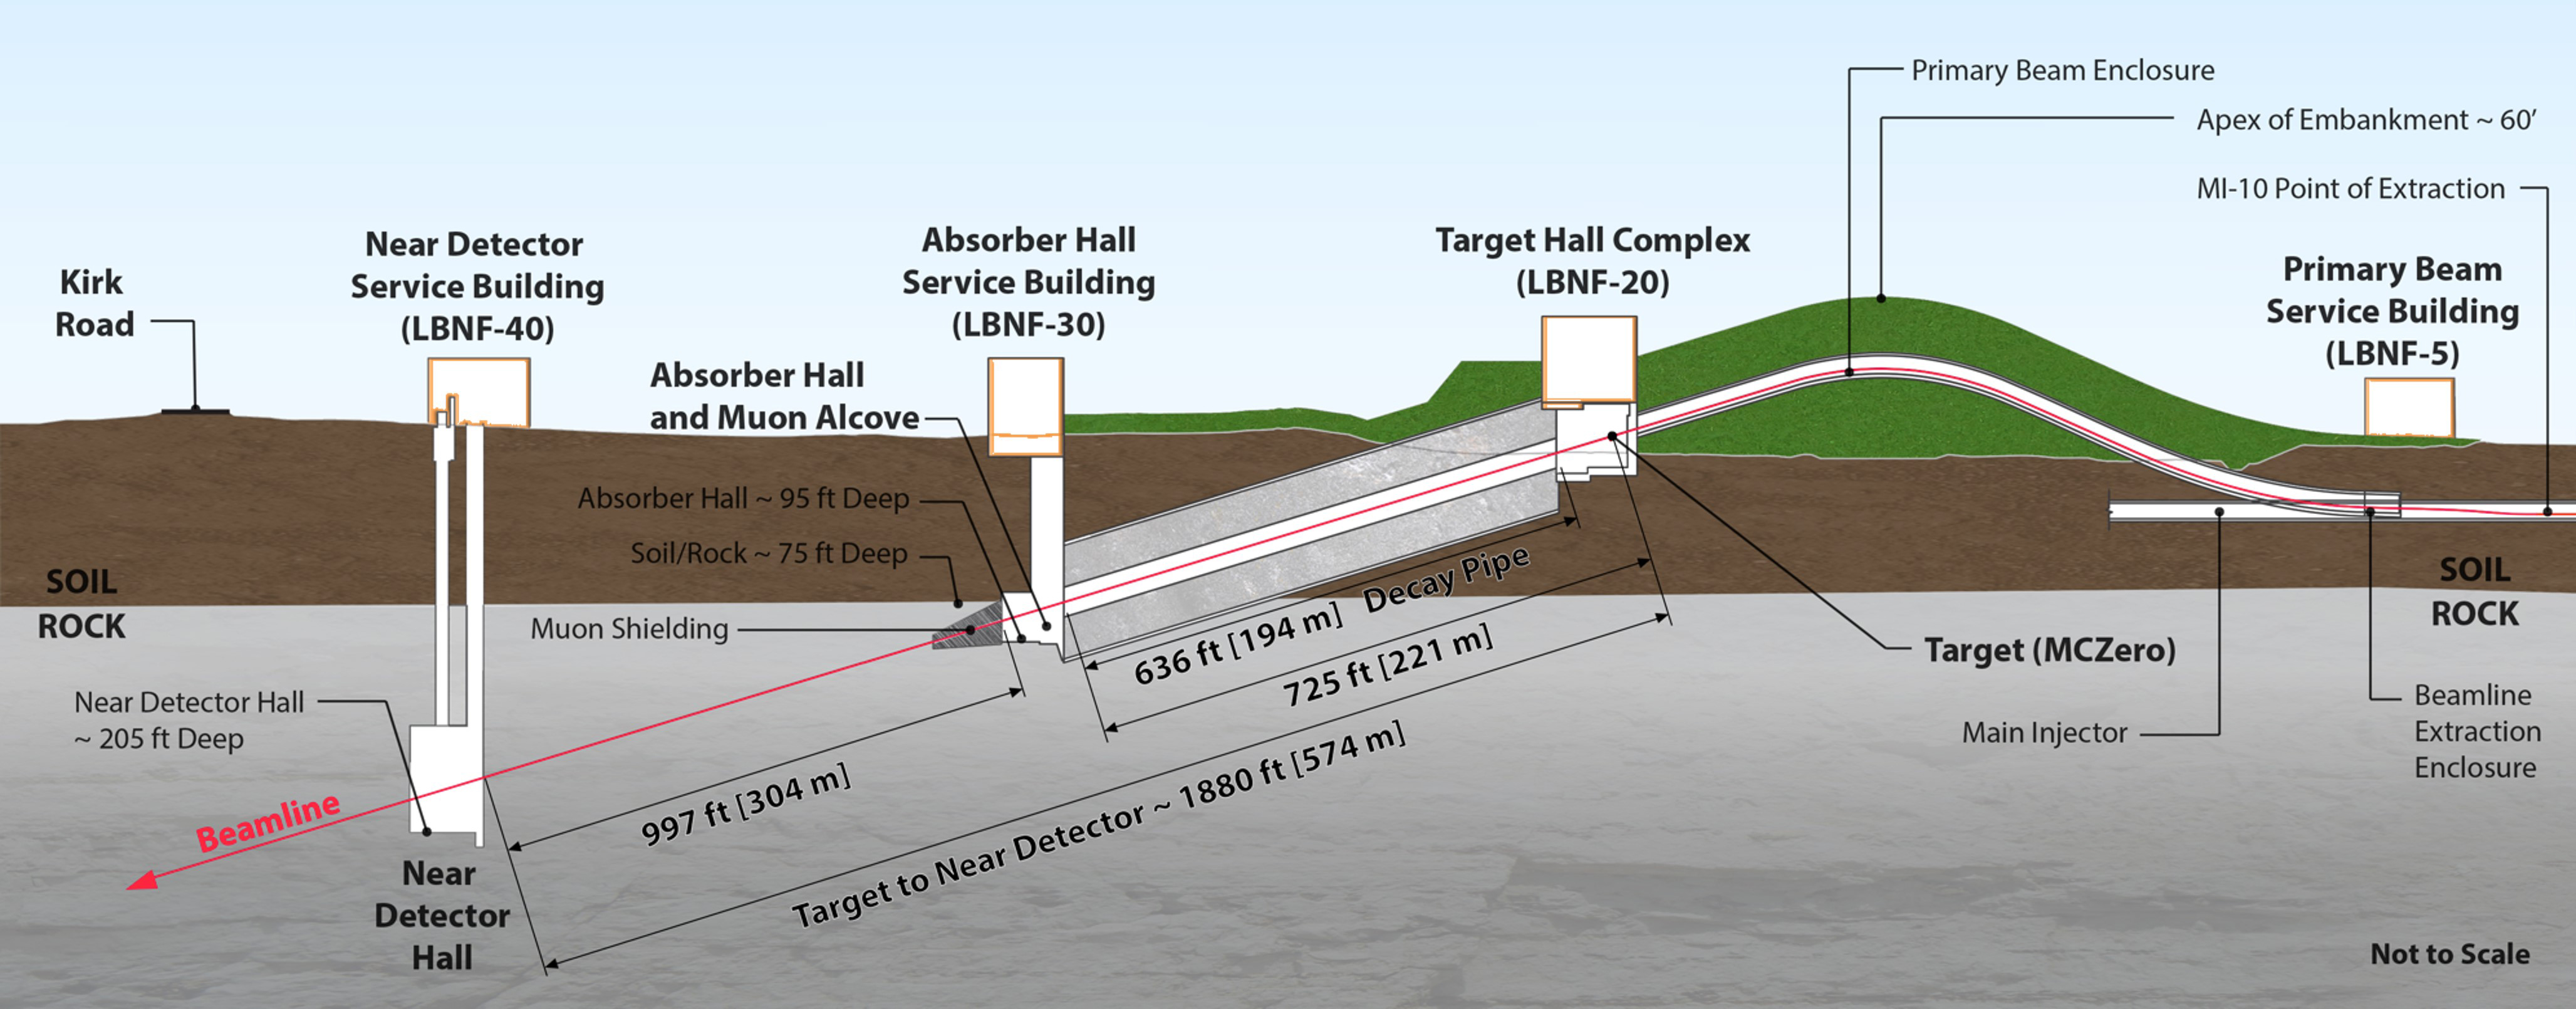
\includegraphics[width=0.8\textwidth]{graphics/i-and-i/near_site_xsec.jpg}
\end{dunefigure}

The Near Detector hall complex consists of a surface building, the underground cavern, and a secondary egress shaft which has a separate air supply for fire safety. A large, \SI{38}{\ft} diameter primary shaft connects the surface building to the cavern and will be utilized for hoisting detector equipment underground. The shaft also accommodates utility and cryogenics lines plus an elevator. Figure~\ref{fig:nd_hall_3d} shows an architectural 3D model and detail drawing of the Near Detector hall complex. Main sizing parameters are summarized in Table~\ref{tab:cavern-sizing-param}.

\begin{dunefigure}[Cavern and surface building architectural drawings]{fig:nd_hall_3d}
{Near Detector cavern and surface building architectural drawings.}
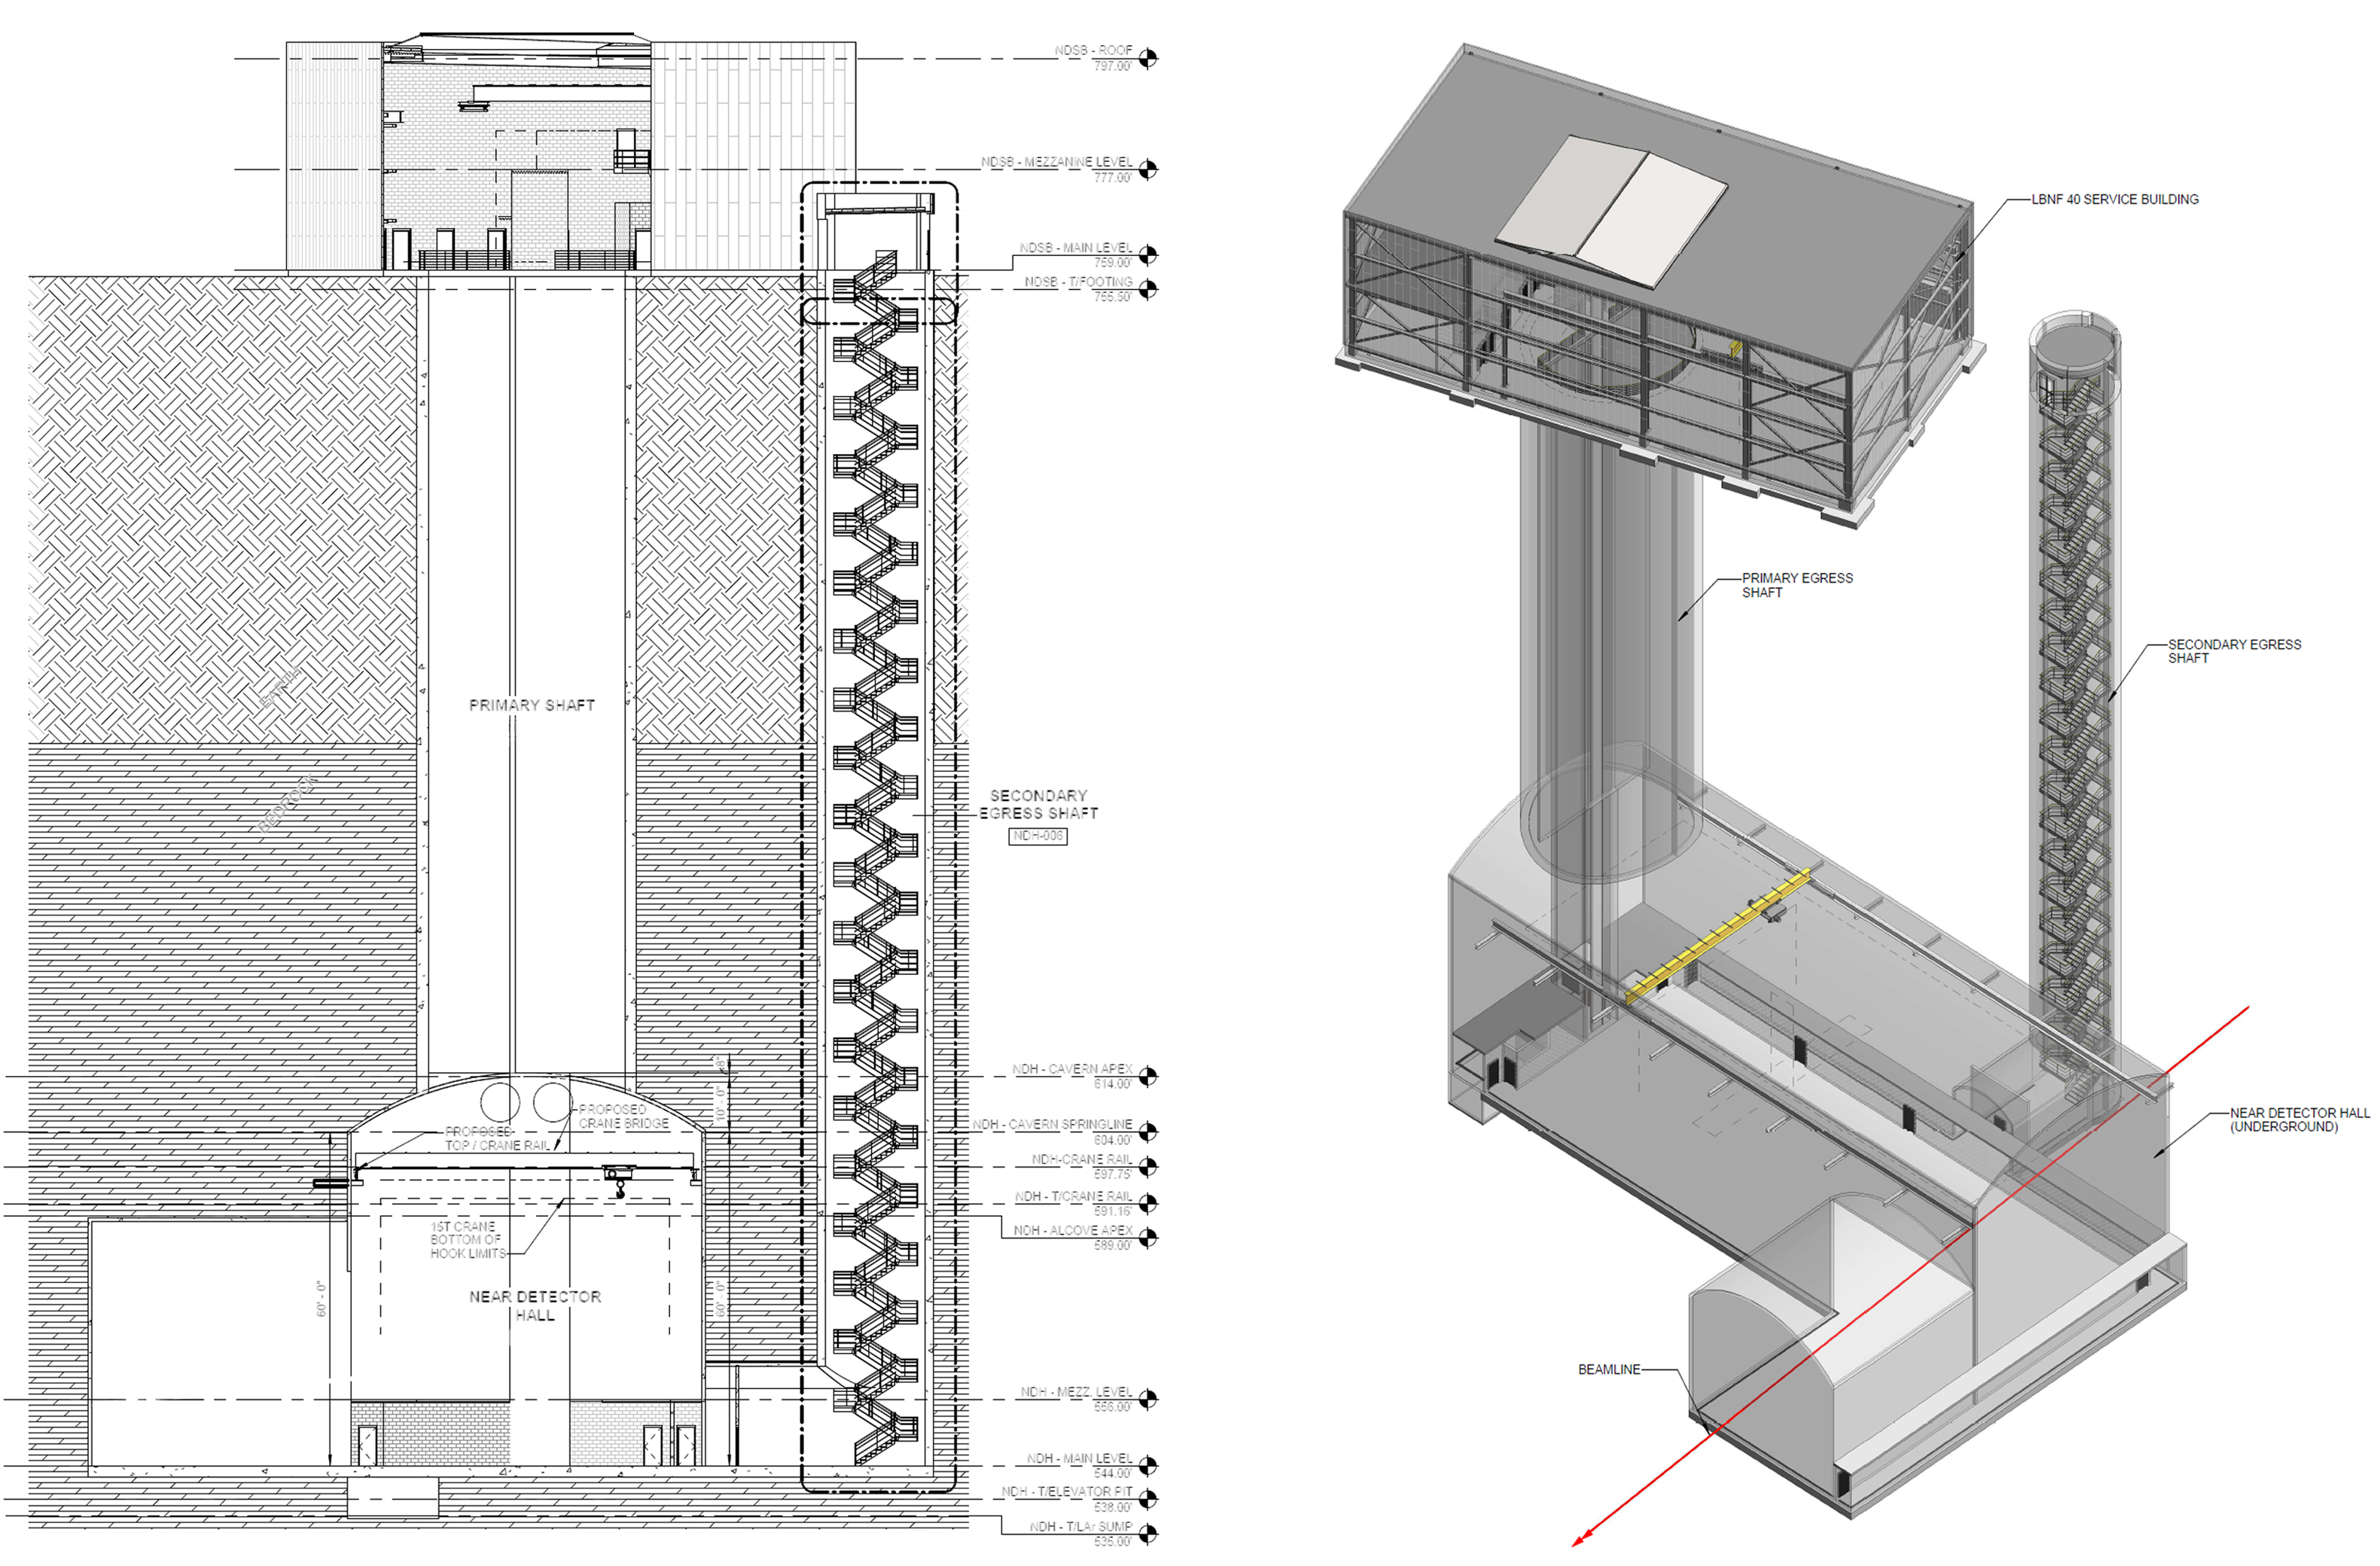
\includegraphics[width=0.8\textwidth]{graphics/i-and-i/nd_hall_3d}
\end{dunefigure}

\begin{dunetable}
[Underground cavern size parameters]
{cc}
{tab:cavern-sizing-param}
{Approximate underground cavern size parameters.}
Cavern Parameter & Dimension \\ \toprowrule
Main Cavern Length & \SI{166}{\ft} \\ \colhline
Main Cavern Width & \SI{63}{\ft} \\ \colhline
Main Cavern Height & $\sim$\SI{50}{\ft} \\ \colhline
Alcove Width & \SI{44}{\ft} - \SI{8}{\in} \\ \colhline
Alcove Depth & \SI{41}{\ft} - \SI{7}{\in} \\ \colhline
Alcove Height & \SI{39}{\ft} \\ \colhline
Access Shaft Clear Diameter & \SI{38}{\ft} \\ % no \colhline on final row
\end{dunetable}

%%%%%%%%%%%%%%%%
\subsection{Detector Arrangement and Neutrino Beamline}
\label{sec:chap-id:introduction:arrangement}

Figure~\ref{fig:nd_detector_arrangement} shows the three ND  subdetectors located at their nominal, on-axis beamline position. The ND-LAr and the ND-GAr subdetectors can move transverse to the neutrino beamline to permit off-axis flux measurements as part of the PRISM science program. PRISM requires an off-axis movement range of approximately \SI{30}{\m}. This distance determines the overall length of the main cavern. On the other hand, the SAND subdetector will act as a stationary, permanent beam monitor at a fixed position inside an alcove along the beam centerline.
 \dword{ndlar} and \dword{ndgar} will typically move together to facilitate the measurements of PRISM, but they can move separately for installation and maintenance as needed.  

\begin{dunefigure}[Cavern layout with ND-LAr, ND-GAr, and SAND detectors]{fig:nd_detector_arrangement}
{Near detector cavern arrangement of the ND-LAr, ND-GAr and SAND subdetectors plus the PRISM movement system.}
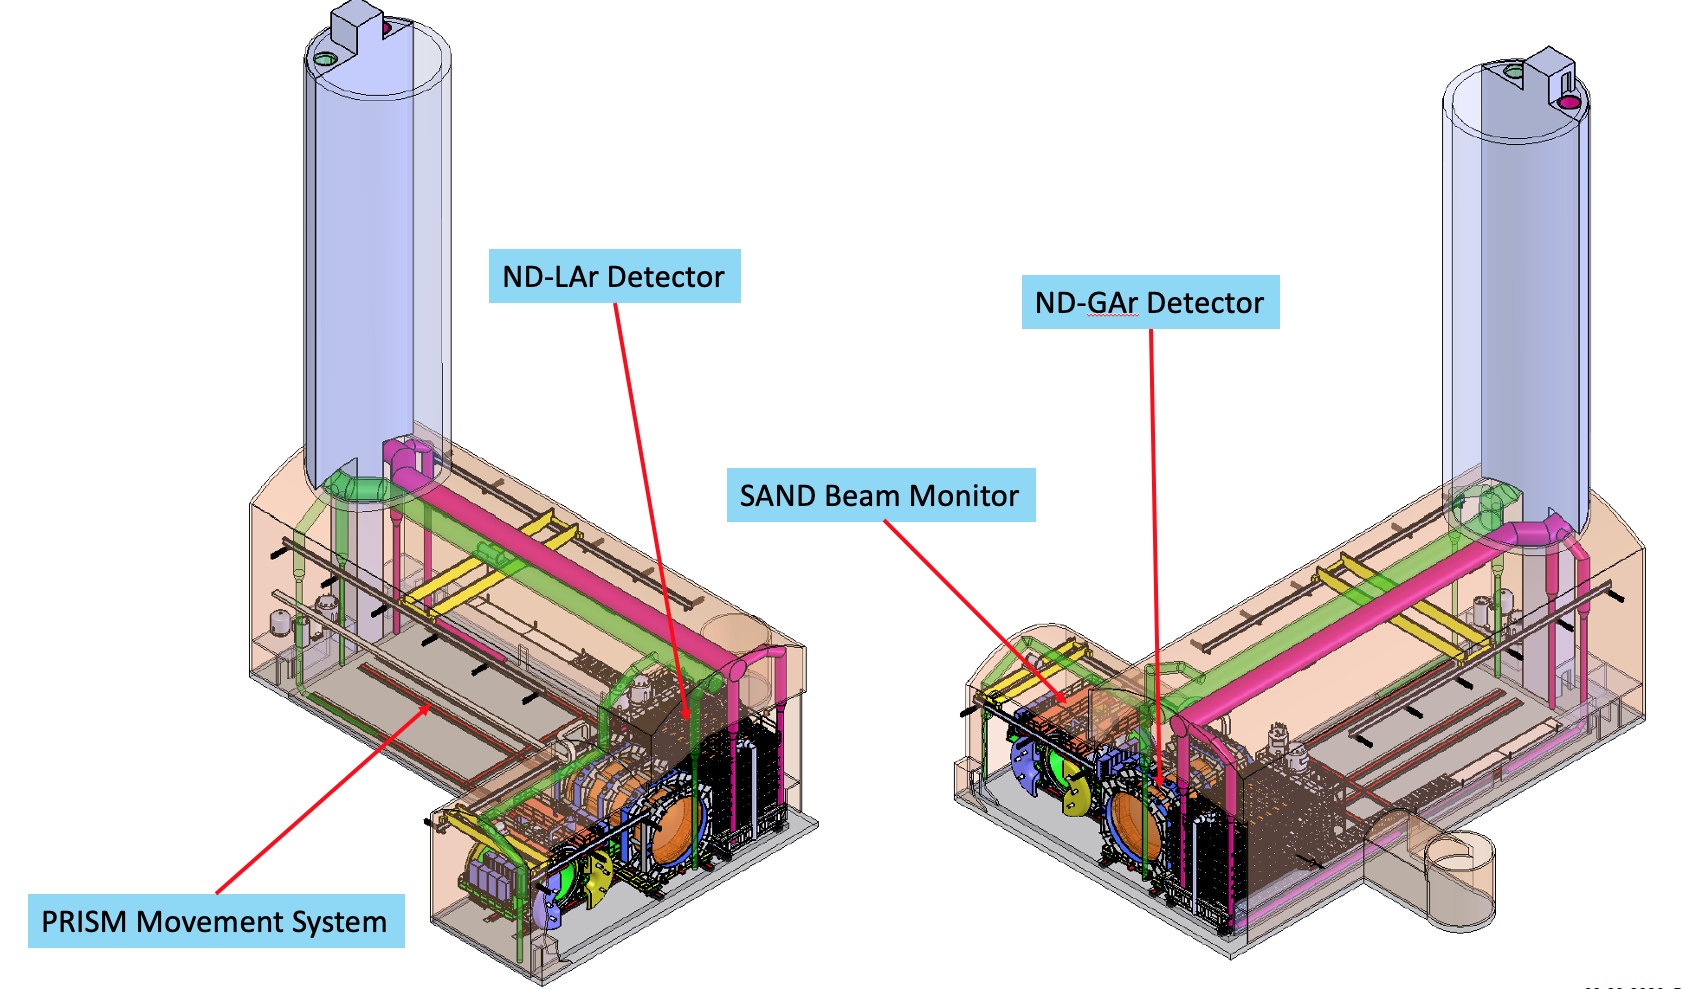
\includegraphics[width=0.9\textwidth]{graphics/i-and-i/nd_detector_arrangement2}
\end{dunefigure}

The neutrino beamline which is directed towards the far site is angled by \SI{5.3}{\degree} with respect to the cavern horizontal plane. As shown in Figure~\ref{fig:beamline} the subdetectors are elevated such that the neutrino beamline passes through the center of the active volume of each subdetector. The figure also summarizes the main dimensions related to the positioning of the detectors inside the cavern.

\begin{dunefigure}[Neutrino beamline location inside the Near Detector cavern]{fig:beamline}
{Near detector positions relative to the cavern and the DUNE neutrino beamline which passes through the center of each detector active volume.}
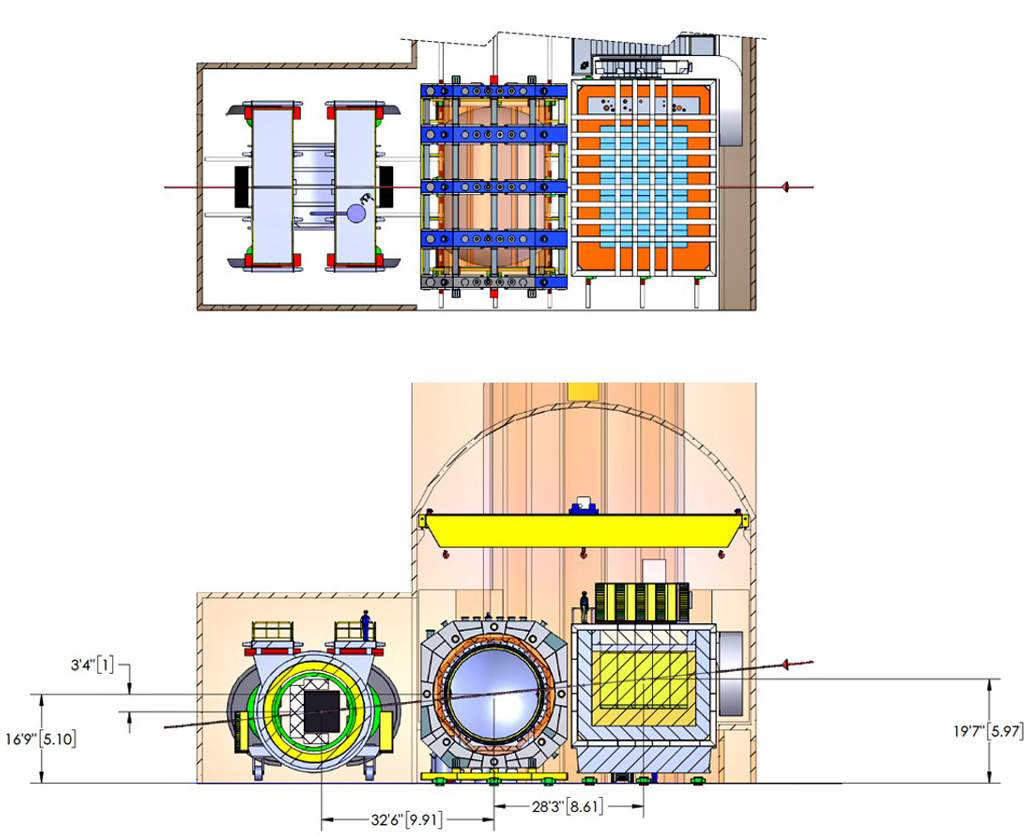
\includegraphics[width=0.9\textwidth]{graphics/i-and-i/beamline}
\end{dunefigure}

The cavern floor consists of a \SI{24}{\in} thick concrete slab resting on the natural rock formation. The structure can support the significant subdetector weights which are summarized in Table~\ref{tab:detector-weights}.

\begin{dunetable}
[approximate detector weights]
{cc}
{tab:detector-weights}
{Approximate subdetector weight summaries.}
%%Detector & \begin{tabular}[x]{@{}c@{}}Approx. Weight\\{[metric ton]}\end{tabular} \\ \toprowrule
Detector & Approximate Weight \\ \toprowrule
ND-LAr Subdetector & \SI{880}{\metricton} \\ \colhline
ND-GAr Subdetector & \SI{710}{\metricton} \\ \colhline
SAND Beam Monitor & \SI{900}{\metricton} \\ \colhline
PRISM & included with detector weights \\ % no \colhline on final row
\end{dunetable}


%%%%%%%%%%%%%%%%%%%%%%%%%%%%%%%% 
\section{ND-LAr Detector Layout and Interfaces}
\label{sec:int-inst-ndlar-layout}

The design configuration for the ND-LAr subdetector setup is shown in Figure~\ref{fig:nd_lar_details}. Seven rows of five pixelated detector modules each (see section~\ref{sec:lartpc-dimensions}) are suspended inside a large membrane cryostat. The design of the membrane cryostat is comparable to similarly sized cryostats built for previous or existing neutrino experiments (ProtoDUNE-SP, for example).

\begin{dunefigure}[Main ND-LAr detector components]{fig:nd_lar_details}
{Image of the ND-LAr subdetector. Seven rows of five pixelated detector modules each are suspended inside a large membrane cryostat. The figure shows prototype module design features which will be adapted to the final cryostat configuration.}
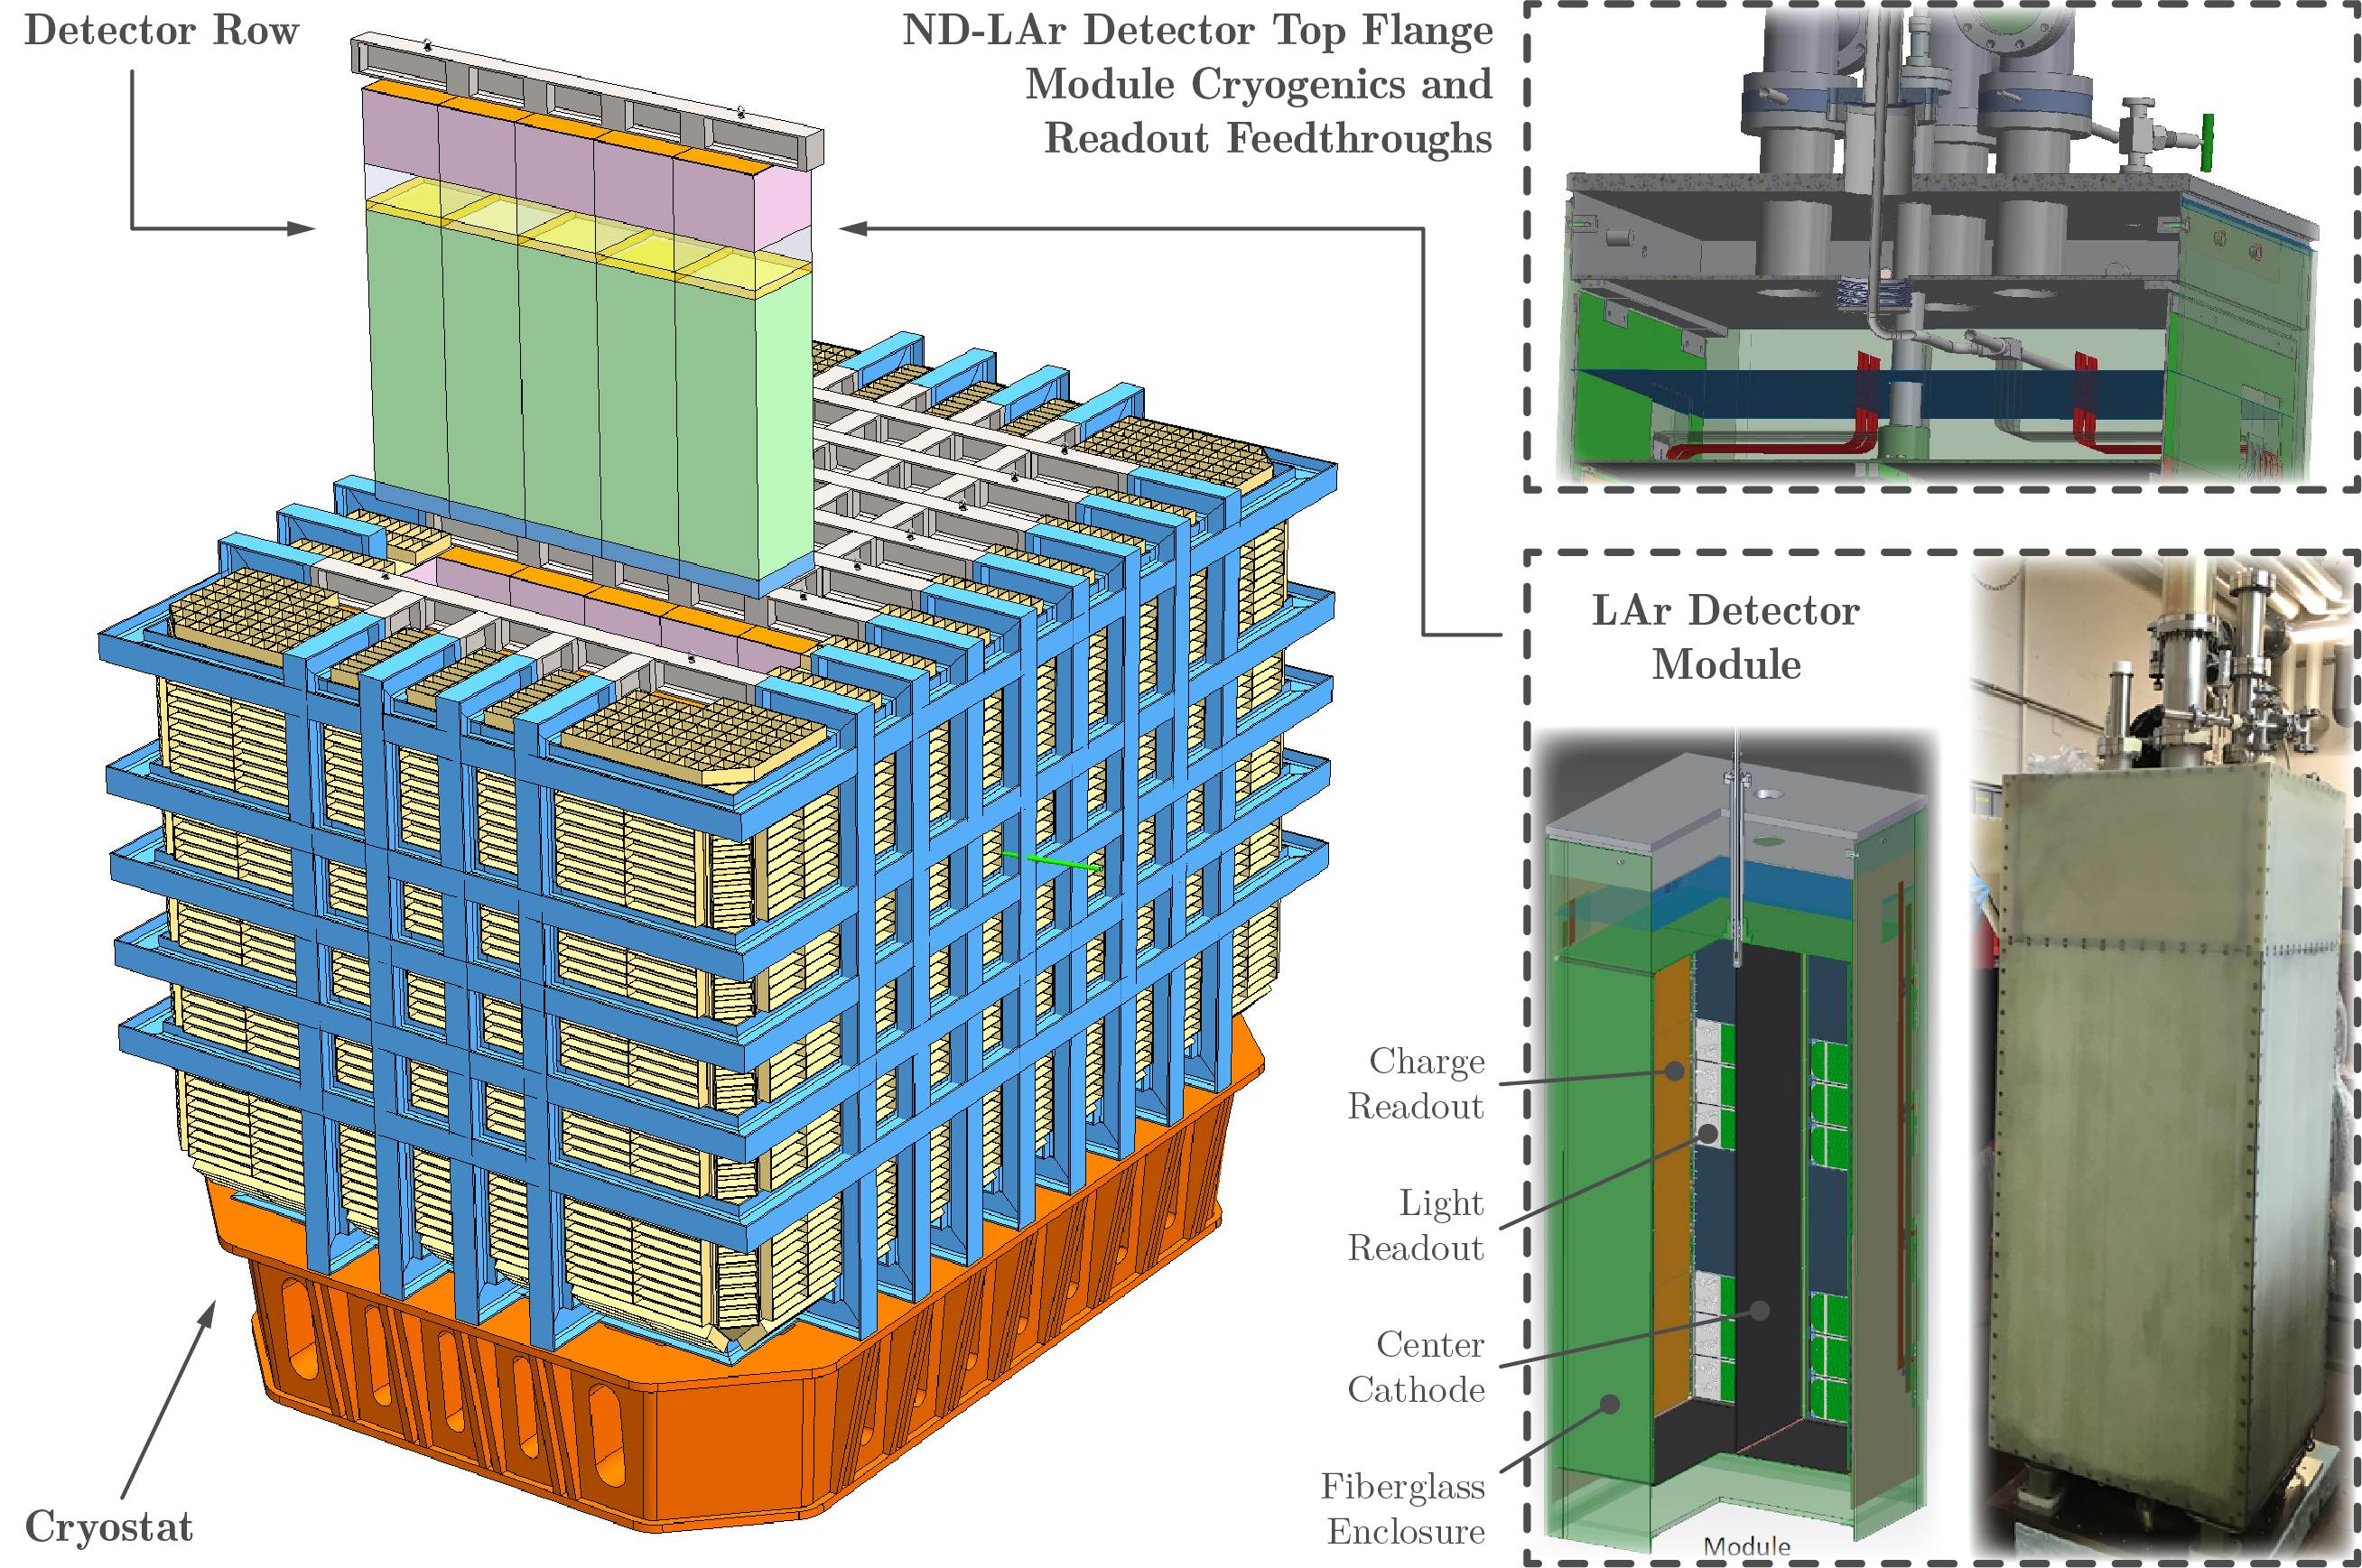
\includegraphics[width=0.8\textwidth]{graphics/i-and-i/nd_lar_details}
\end{dunefigure}

The cryostat stores roughly \SI{300}{\metricton}s of liquid argon, and its outside dimensions are approximately \SI{11.4}{\m} wide (transverse to neutrino beam) x \SI{8.4}{\m} deep (along neutrino beam) x \SI{7.0}{\m} high. \begin{comment}A cryogenic process flow diagram for the ND-LAr subdetector is shown in Figure~\ref{fig:nd_lar_flowdiagram}.\end{comment} A unique feature of the subdetector will be a large cable carrier (see Figure~\ref{fig:nd_lar_setup}) which houses flexible cryogenic pipes, power, and data acquisition cables. To minimize the quantity of flexible cryogenic piping in the cable carrier most of the argon purification system will be located on a two-level support system mounted on the moveable detector platform. The argon cryogenic system will be designed based on extensive experiences on ProtoDUNE enabling optimization of space needs on the detector platform.

\begin{comment}
\begin{dunefigure}[ND-LAr cryogenic process flow diagram]{fig:nd_lar_flowdiagram}
{Cryogenic process flow diagram for the ND-LAr subdetector. A unique feature of the ND-LAr detector will be the capability of moving the entire cryogenic purification system together with the detector for off-axis beam measurements.}
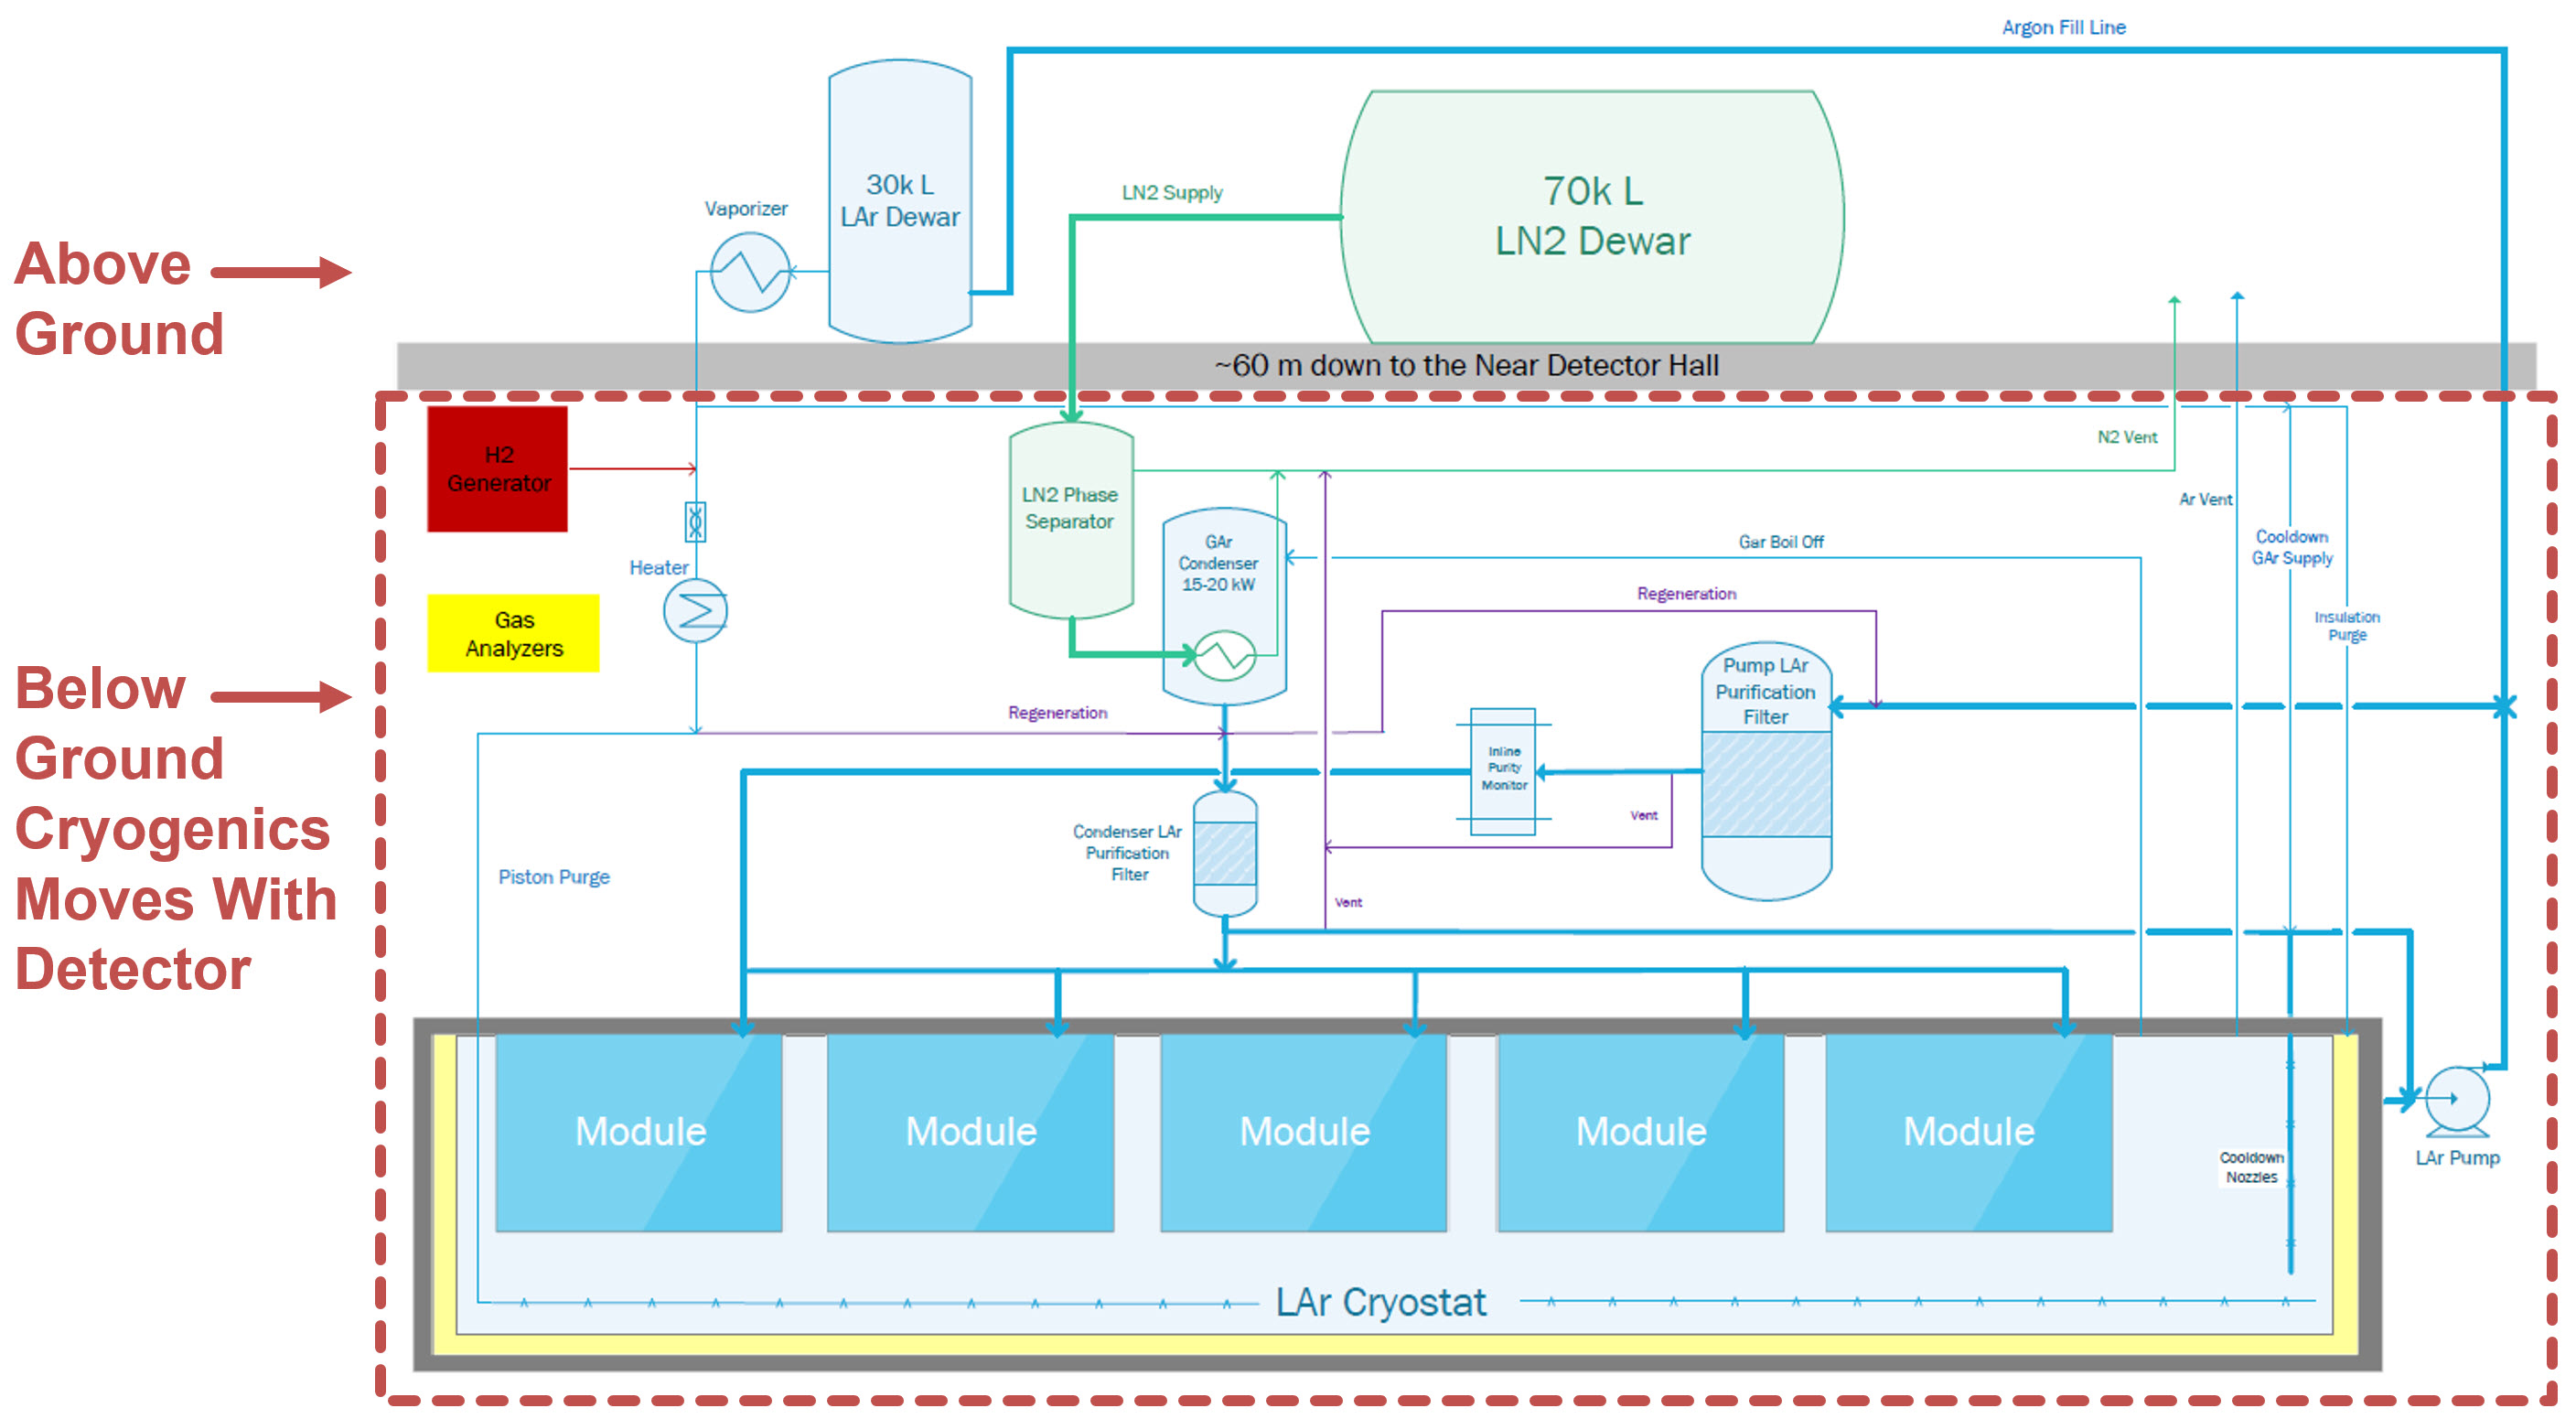
\includegraphics[width=0.8\textwidth]{graphics/i-and-i/nd_lar_flowdiagram}
\end{dunefigure}
\end{comment}

\begin{dunefigure}[Detailed ND-LAr detector layout]{fig:nd_lar_setup}
{Illustration of the ND-LAr subdetector setup including the cryostat, the cryogenic purification system, and the PRISM movement system. A large cable carrier houses flexible cryogenic pipes, power, and data acquisition cables. \dword{ndgar} will have a similar, separate cable carrier.}
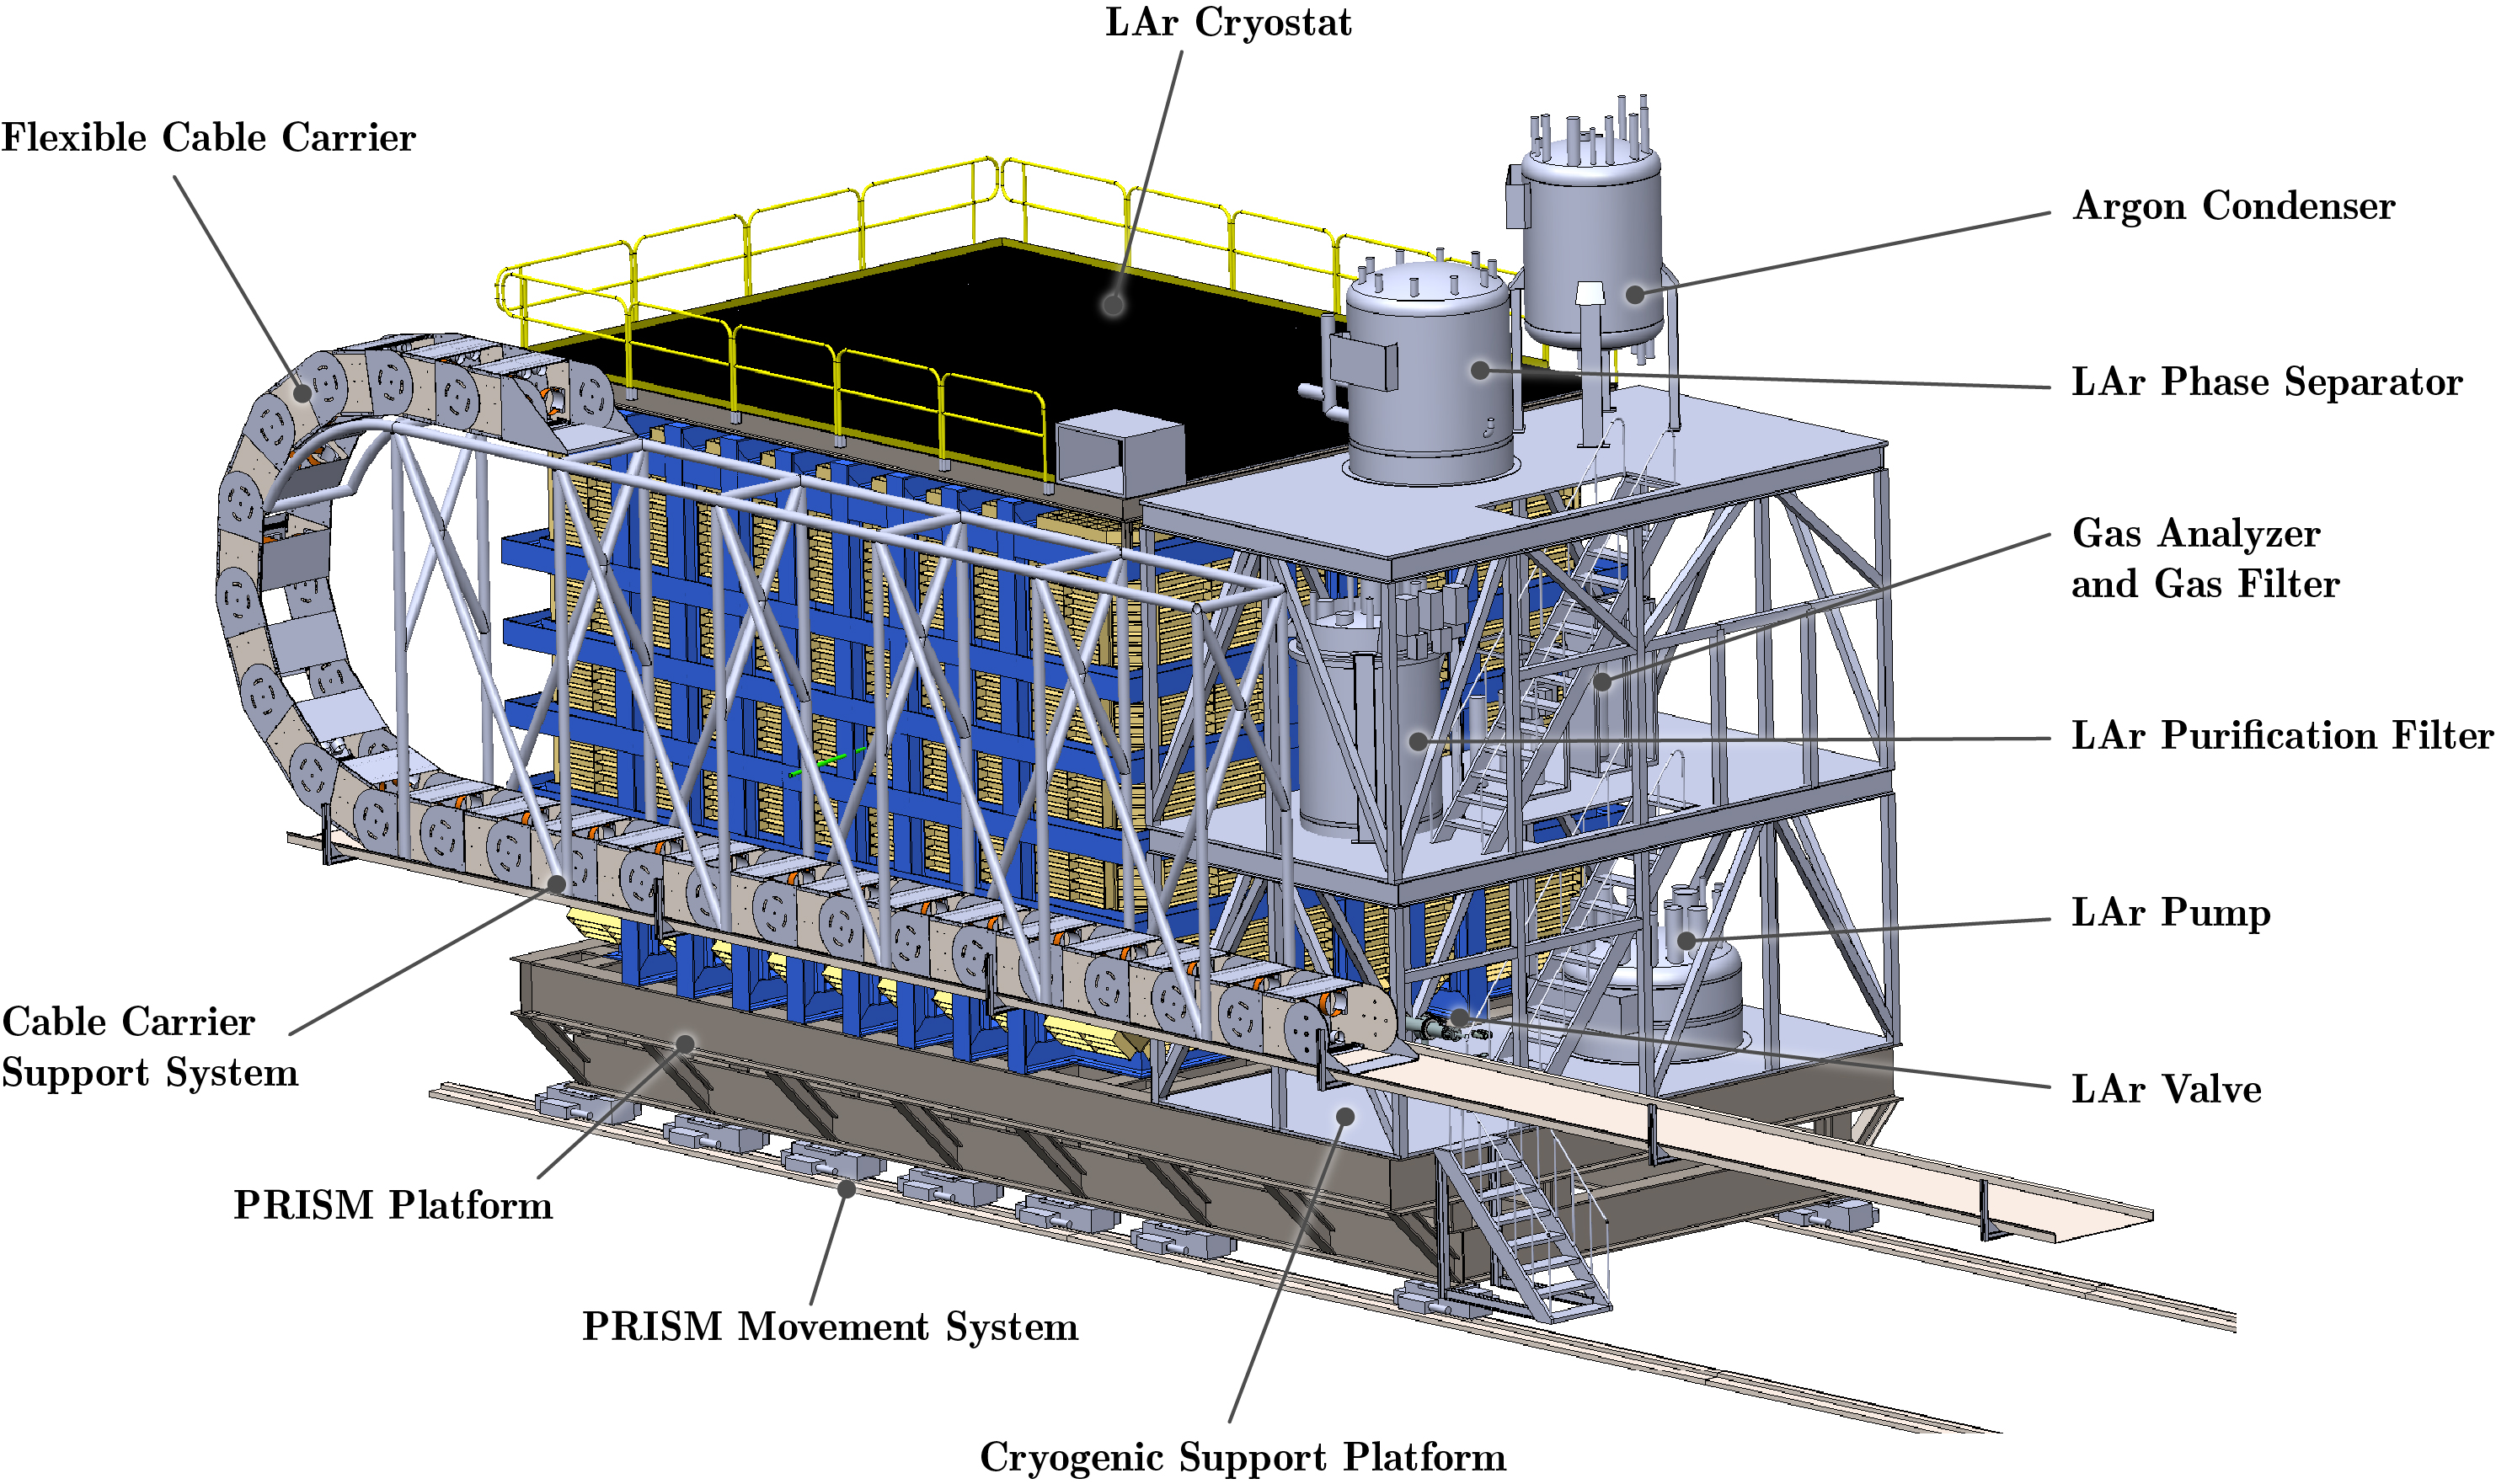
\includegraphics[width=0.8\textwidth]{graphics/i-and-i/nd_lar_setup}
\end{dunefigure}

The ND-LAr subdetector, which can only contain muons with energies up to approximately \SI{1}{\GeV}, needs to operate in conjunction with the ND-GAr subdetector (see section \ref{sec:chap-id:details:mpd}) to cover the full muon energy spectrum up to approximately \SI{5}{\GeV}. Passive material between the ND-LAr and the ND-GAr subdetectors must be minimized in order to maximize the muon detection efficiency. Therefore, the LAr cryostat is designed to include a large, low-mass fiberglass back-wall which is designed to interlock with the main steel beams of the cryostat.


%%%%%%%%%%%%%%%%%%%%%%%%%%%%%%%% 
\section{TMS Detector Layout and Interfaces}
\label{sec:int-inst-tms-layout}

\begin{dunefigure}[TMS detector layout]{fig:tms_setup}
{Illustration of the TMS subdetector setup.}
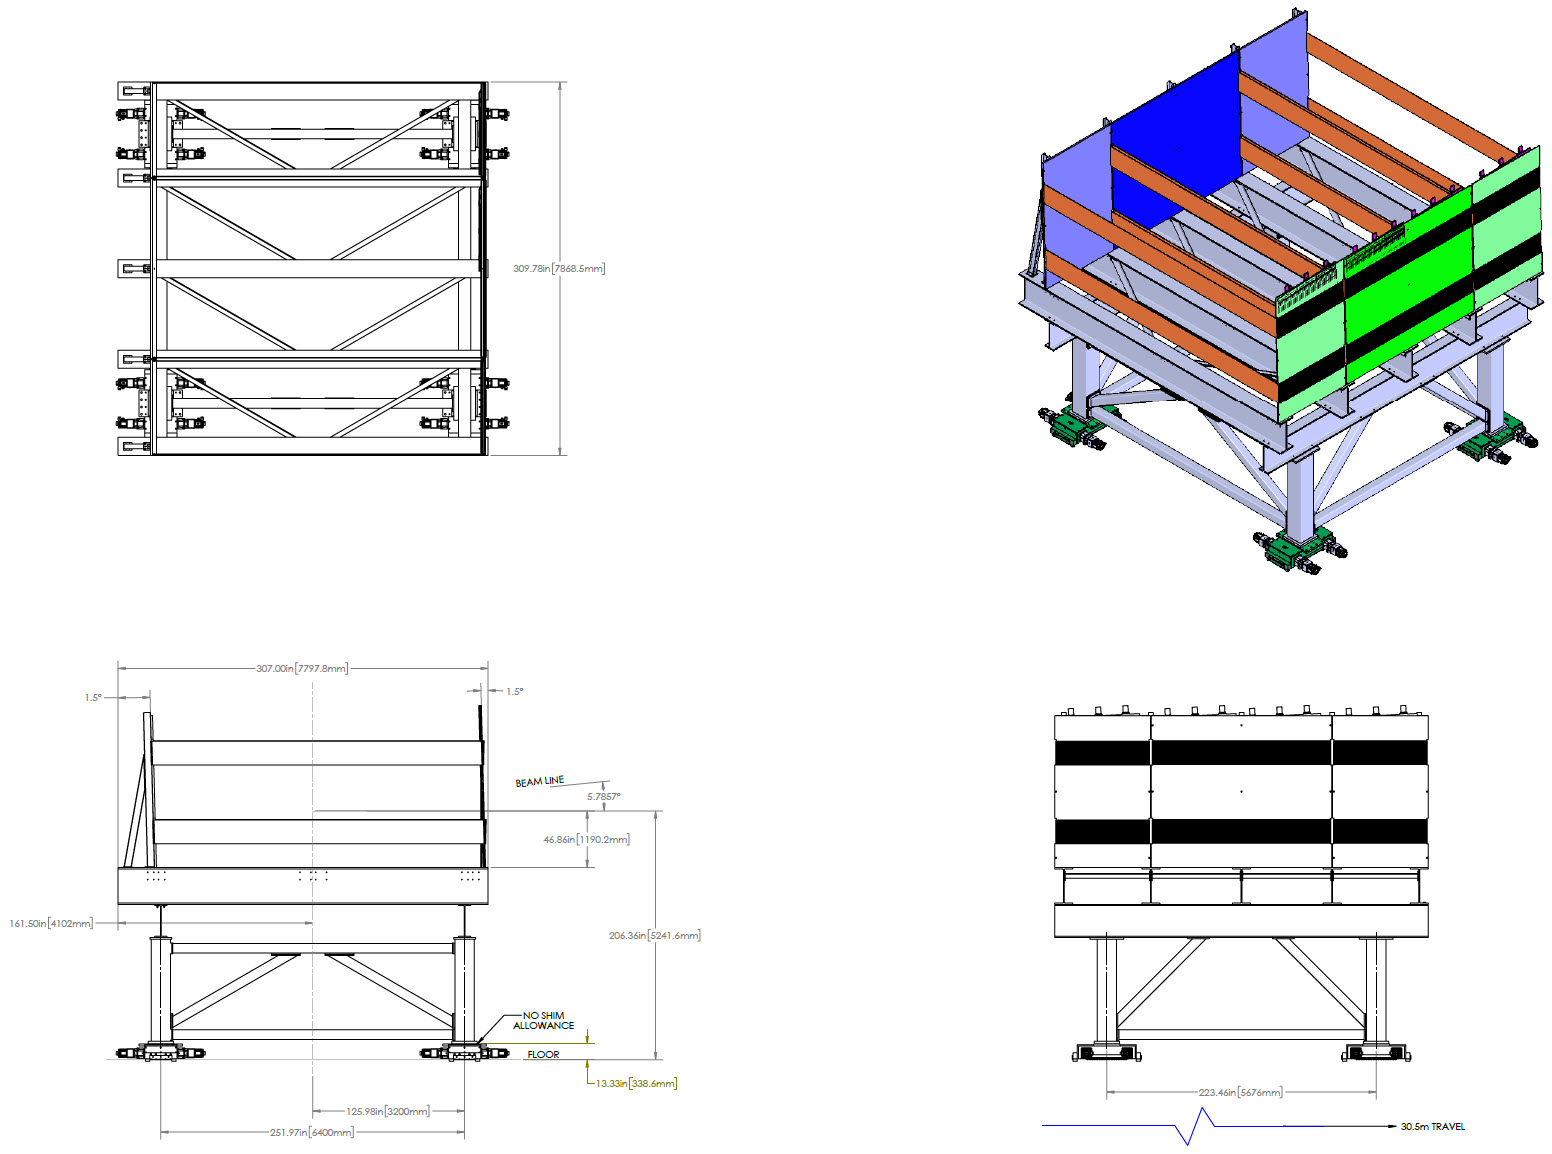
\includegraphics[width=0.8\textwidth]{graphics/i-and-i/tms_setup}
\end{dunefigure}


%%%%%%%%%%%%%%%%%%%%%%%%%%%%%%%% 
\section{SAND Detector Layout and Interfaces}
\label{sec:int-inst-sand-layout}

The \dword{nd} cavern includes an alcove to house a stationary beam monitor for continuous flux measurements, since ND-LAr  and ND-GAr are designed to be moved off-axis. An existing collider detector structure (KLOE, which is currently installed at INFN Frascati, Italy, see Figure~\ref{fig:sand_photos}) will provide the magnet system and ECAL for SAND. As shown in Figure~\ref{fig:sand_schematic}, SAND consists of a large superconducting solenoid which produces approximately \SI{0.6}{\T} on-axis field. The magnetic field is uniform over a large volume inside the subdetector due to a carefully designed and heavy steel yoke including large end plates which can be opened for access. The main magnet parameters are summarized in Table~\ref{tab:sand_coil_data}. The fully assembled subdetector has an approximately length of \SI{10}{\m} and height of \SI{11}{\m}.

\begin{dunefigure}[SAND detector installation photos]{fig:sand_photos}
{Parts of an existing detector (KLOE, which is currently installed at INFN Frascati, Italy) will be repurposed for use in the SAND beam monitor.}
\includegraphics[width=0.7\textwidth]{graphics/i-and-i/sand_photos}
\end{dunefigure}

The SAND subdetector comes with a lead-scintillating fiber calorimeter with photomultiplier readout. The central barrel has an inner diameter of \SI{4}{\m}, \SI{4.3}{\m} active length, and \SI{23}{\cm} thickness. Two calorimeter end caps as shown in Figure~\ref{fig:sand_schematic} close the barrel. The total weight of the calorimeter is approximately \SI{110}{\metricton}. The innermost diagnostic components, which must fit within the existing KLOE TPC volume constraints, are still in design development and will be based on 3DST, TPC, or straw tube technology.

\begin{dunefigure}[Detailed SAND beam monitor layout]{fig:sand_schematic}
{Schematic drawing of the primary SAND beam monitor components. The subdetector consists of a large superconducting coil surrounded by a thick iron yoke and end plates which produce a uniform magnetic field within the subdetector volume. The subdetector incorporates a lead-based electromagnetic calorimeter barrel. The detailed inner detector design is still ongoing and will be based on either 3DST, TPC, or straw tube technology.}
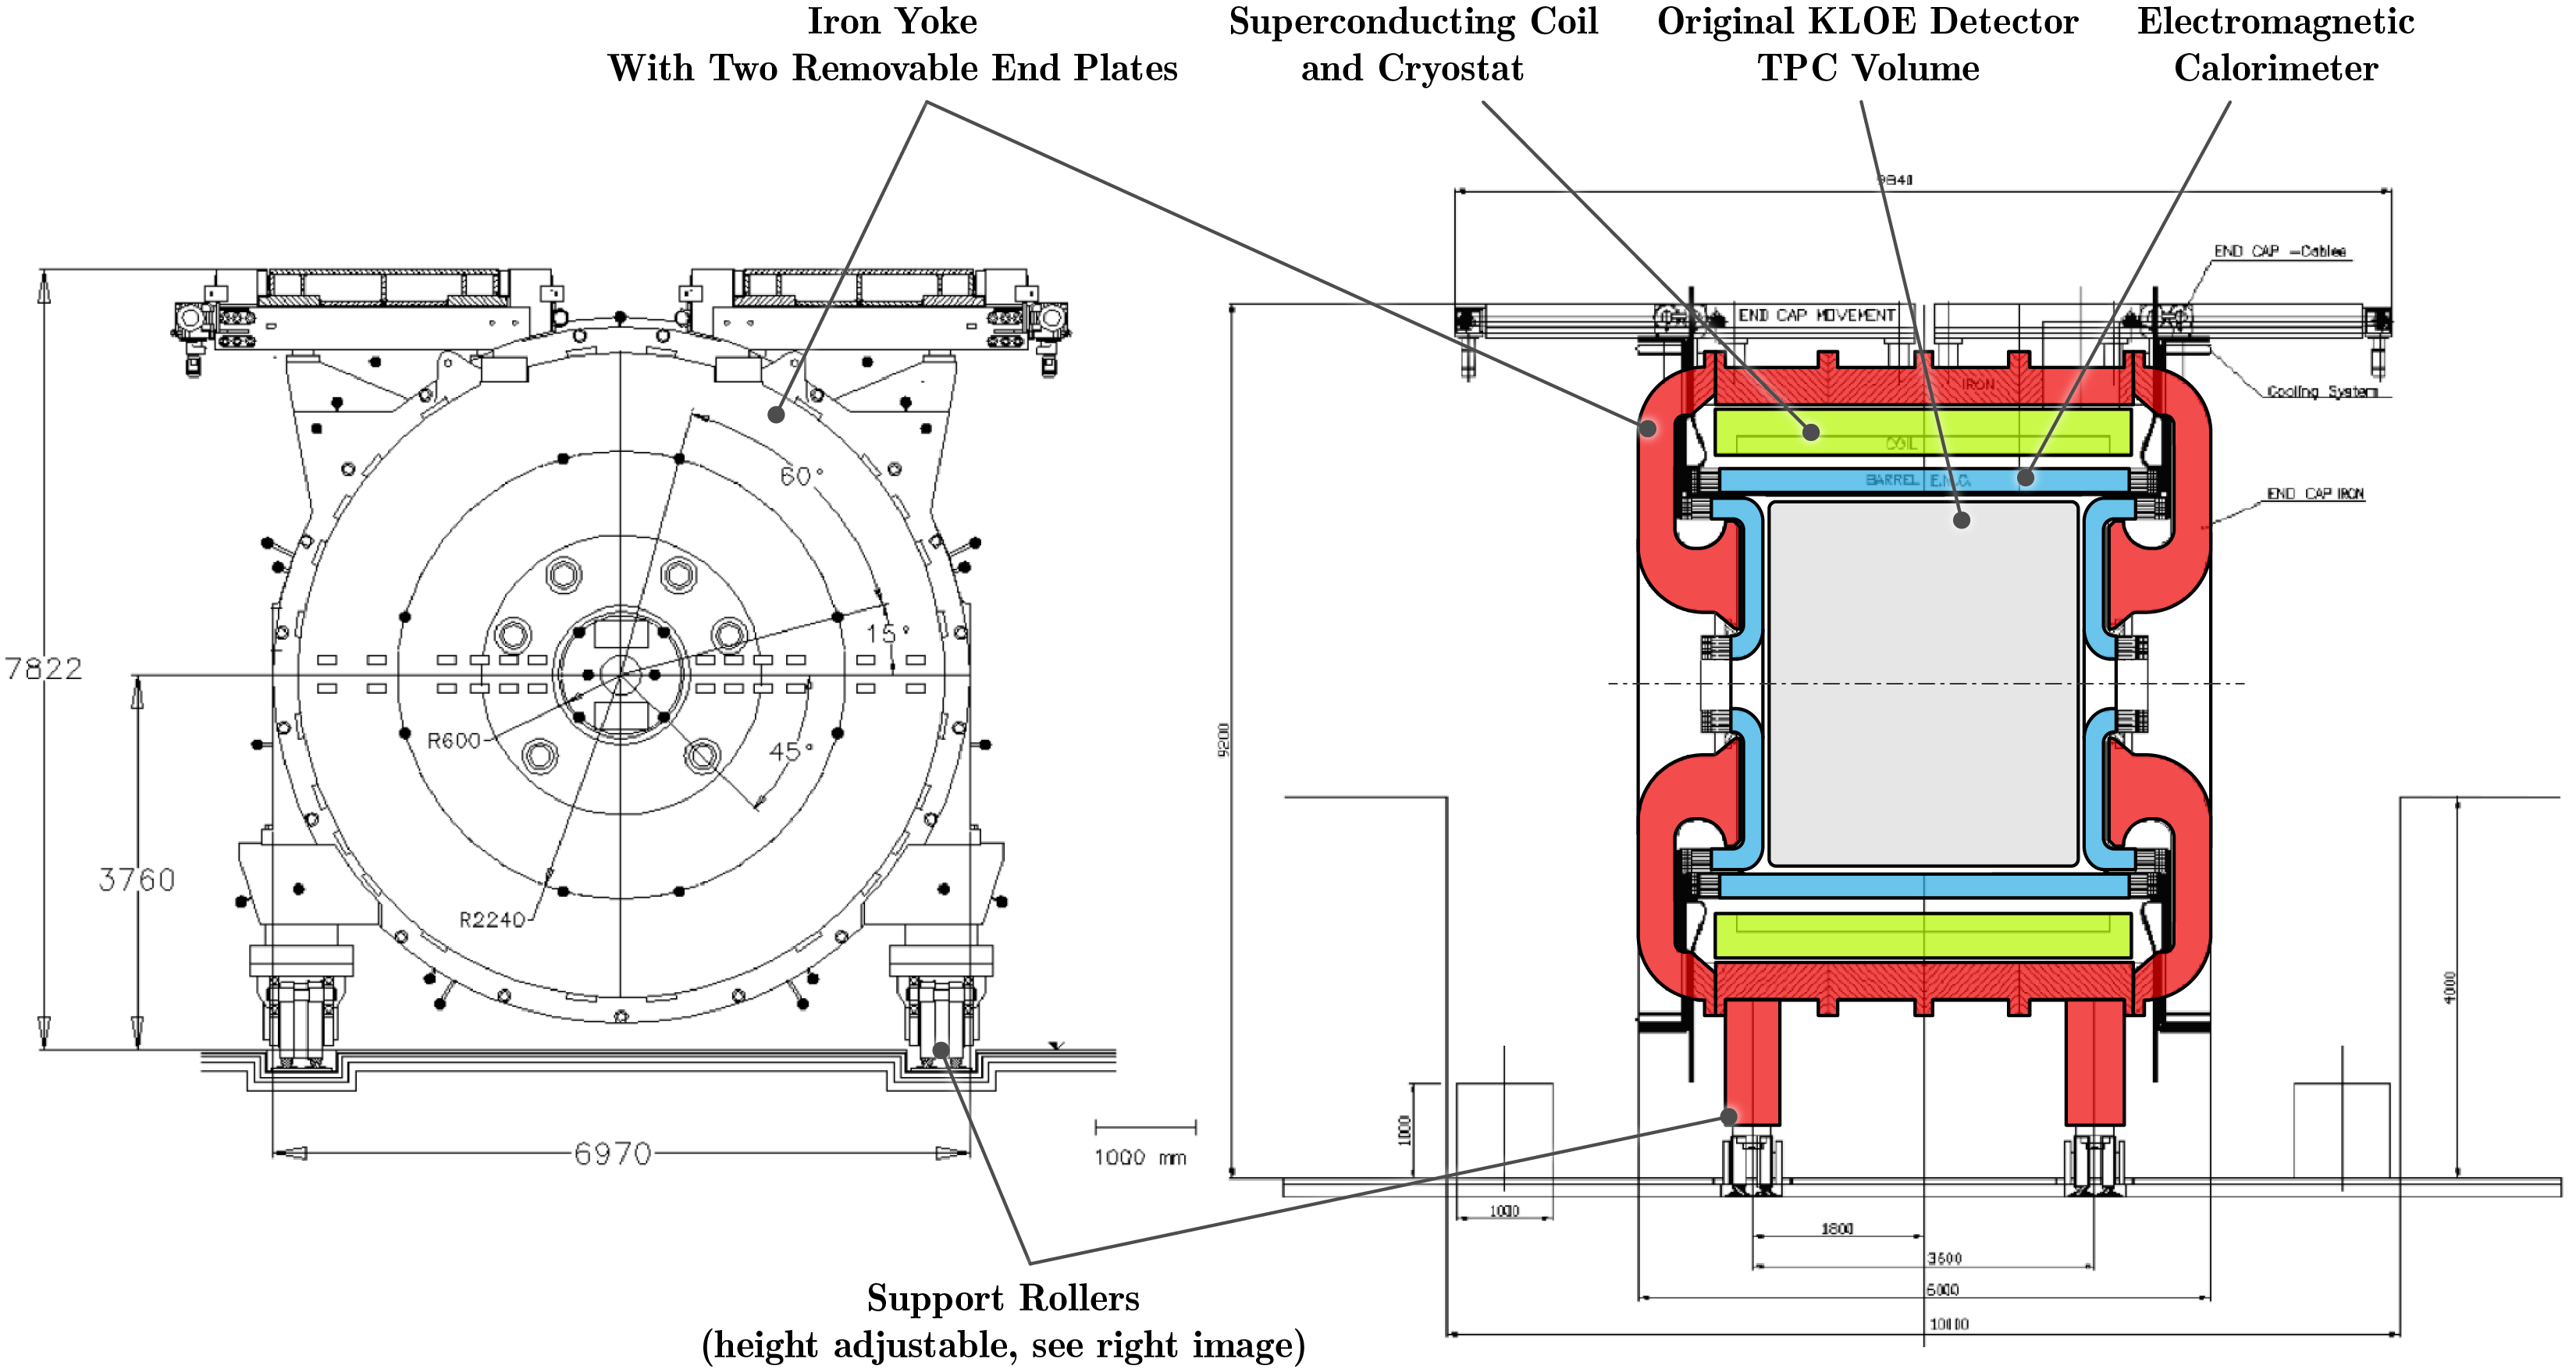
\includegraphics[width=0.8\textwidth]{graphics/i-and-i/sand_schematic}
\end{dunefigure}

\begin{dunetable}
[SAND magnet parameters]
{cc}
{tab:sand_coil_data}
{Important SAND magnet parameters.}
Parameter & Quantity \\ \toprowrule
Central Magnetic Field & \SI{0.6}{\T} \\ \colhline
Solenoid Coil Inner Diameter & \SI{5.19}{\m} \\ \colhline
Cryostat Inner Diameter & \SI{4.86}{\m} \\ \colhline
Cryostat Outer Diameter & \SI{5.76}{\m} \\ \colhline
Cryostat Length & \SI{4.4}{\m} \\ \colhline
Coldmass and Cryostat Weight & \SI{36}{\metricton} \\ \colhline
Iron Return Yoke Weight & \SI{475}{\metricton} \\ \colhline
Operating Current & \SI{2902}{\A} \\ \colhline
Stored Energy & \SI{14.3}{\MJ} \\ % no \colhline on final row
\end{dunetable}

The SAND beam monitor requires the installation of a cryoplant in the Near Detector facility. The superconducting coil is cooled by liquid helium supplied at 1.2~bar and 1.44~K, and the cryostat thermal shield is cooled by 70-80~K gaseous helium. The cooling requirements for SAND are modest, with a heat load to 4~K of less than 55~W, a heat load to the 70~K thermal intercepts of less than 530~W, and a helium flow along the current leads of 0.6~g/s. A small, commercially available cryoplant (approximately 200~W cooling capacity at 4.5~K) will be sufficient for SAND. Its coldbox can be located underground in the vicinity of the shaft as shown in Figure~\ref{fig:sand_cryo_location}. The plant compressor and oil removal skid will be located above ground in the surface support building (see section \ref{sec:chap-id:facility:surface}). The cryoplant requires liquid nitrogen for pre-cooling. The liquid nitrogen cryogenic system including a liquid nitrogen phase separator can be shared between the SAND liquid helium and the ND-LAr argon purification systems.

\begin{dunefigure}[SAND cryoplant location]{fig:sand_cryo_location}
{A small, commercially available cryoplant will be sufficient to cool the SAND superconducting solenoid. Its coldbox can be located underground in the vicinity of the shaft.}
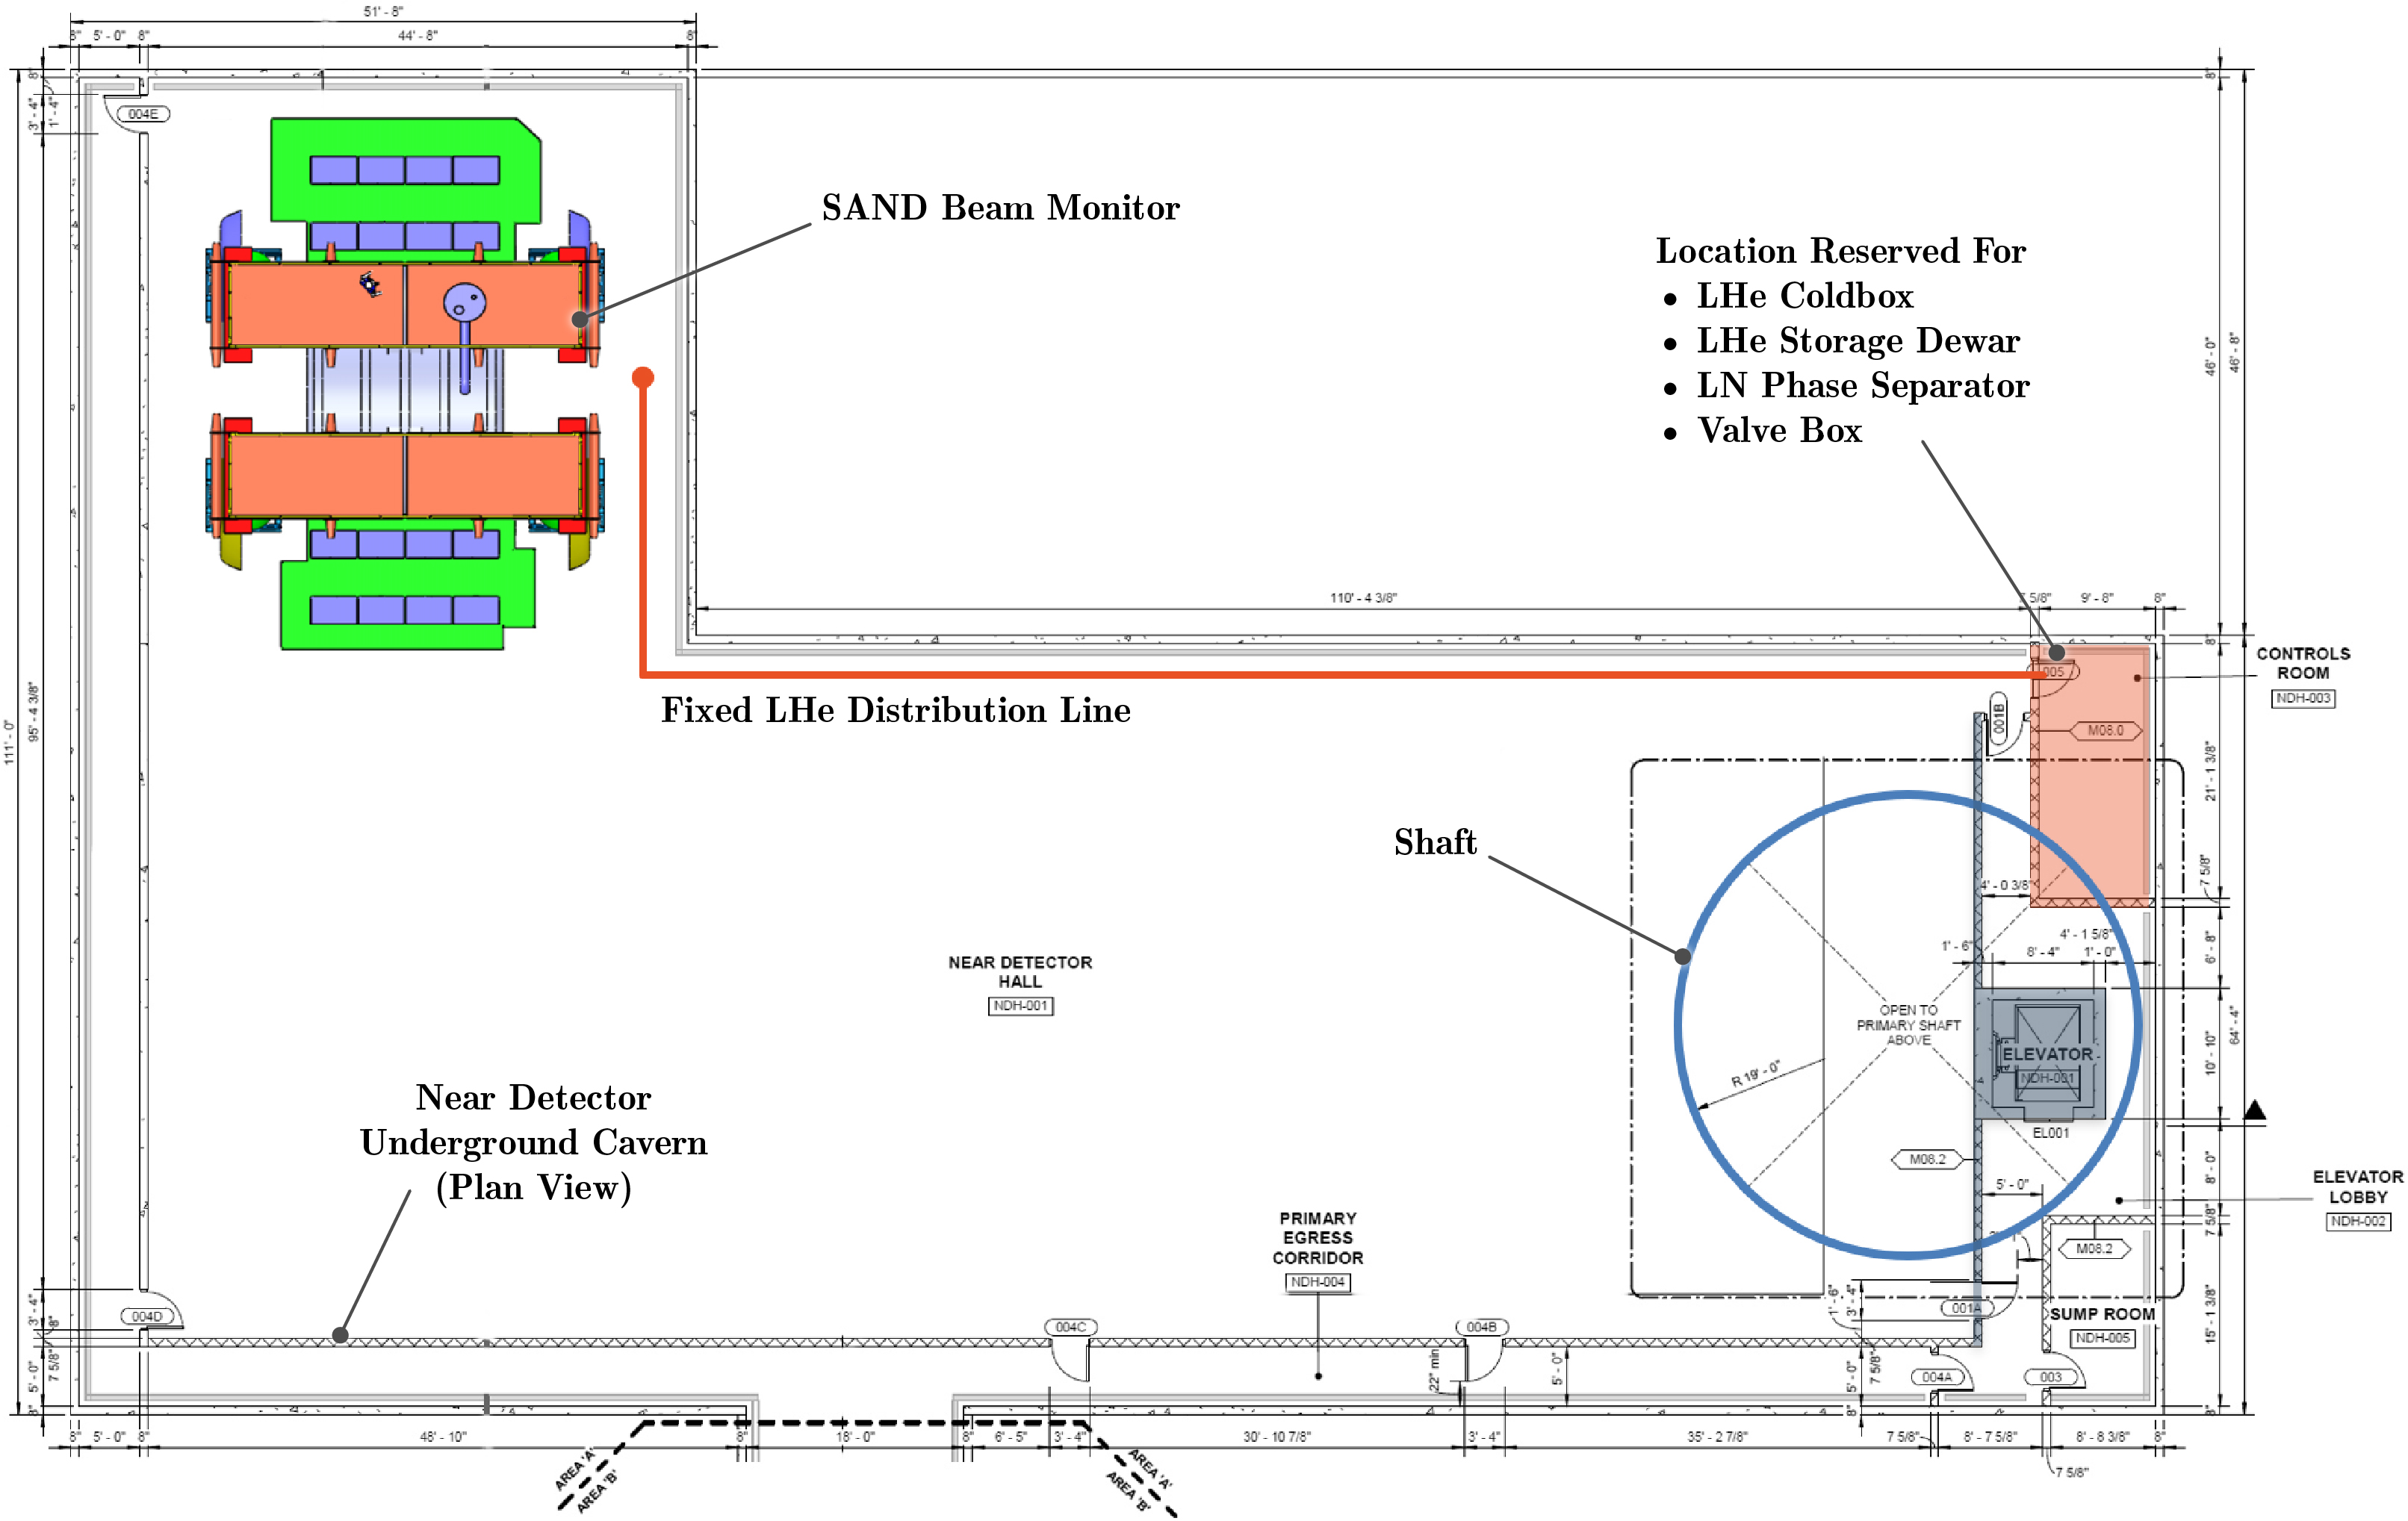
\includegraphics[width=0.8\textwidth]{graphics/i-and-i/sand_cryo_location}
\end{dunefigure}

\begin{dunefigure}[SAND support and movement system]{fig:sand_installation}
{SAND incorporates a versatile support system with large diameter steel rollers for smooth movement and a specialized hydraulic system to adjust the detector height. The steel rollers can be rotated by \SI{90}{\degree} which permits movement of the beam monitor from its assembly area to the final alcove location.}
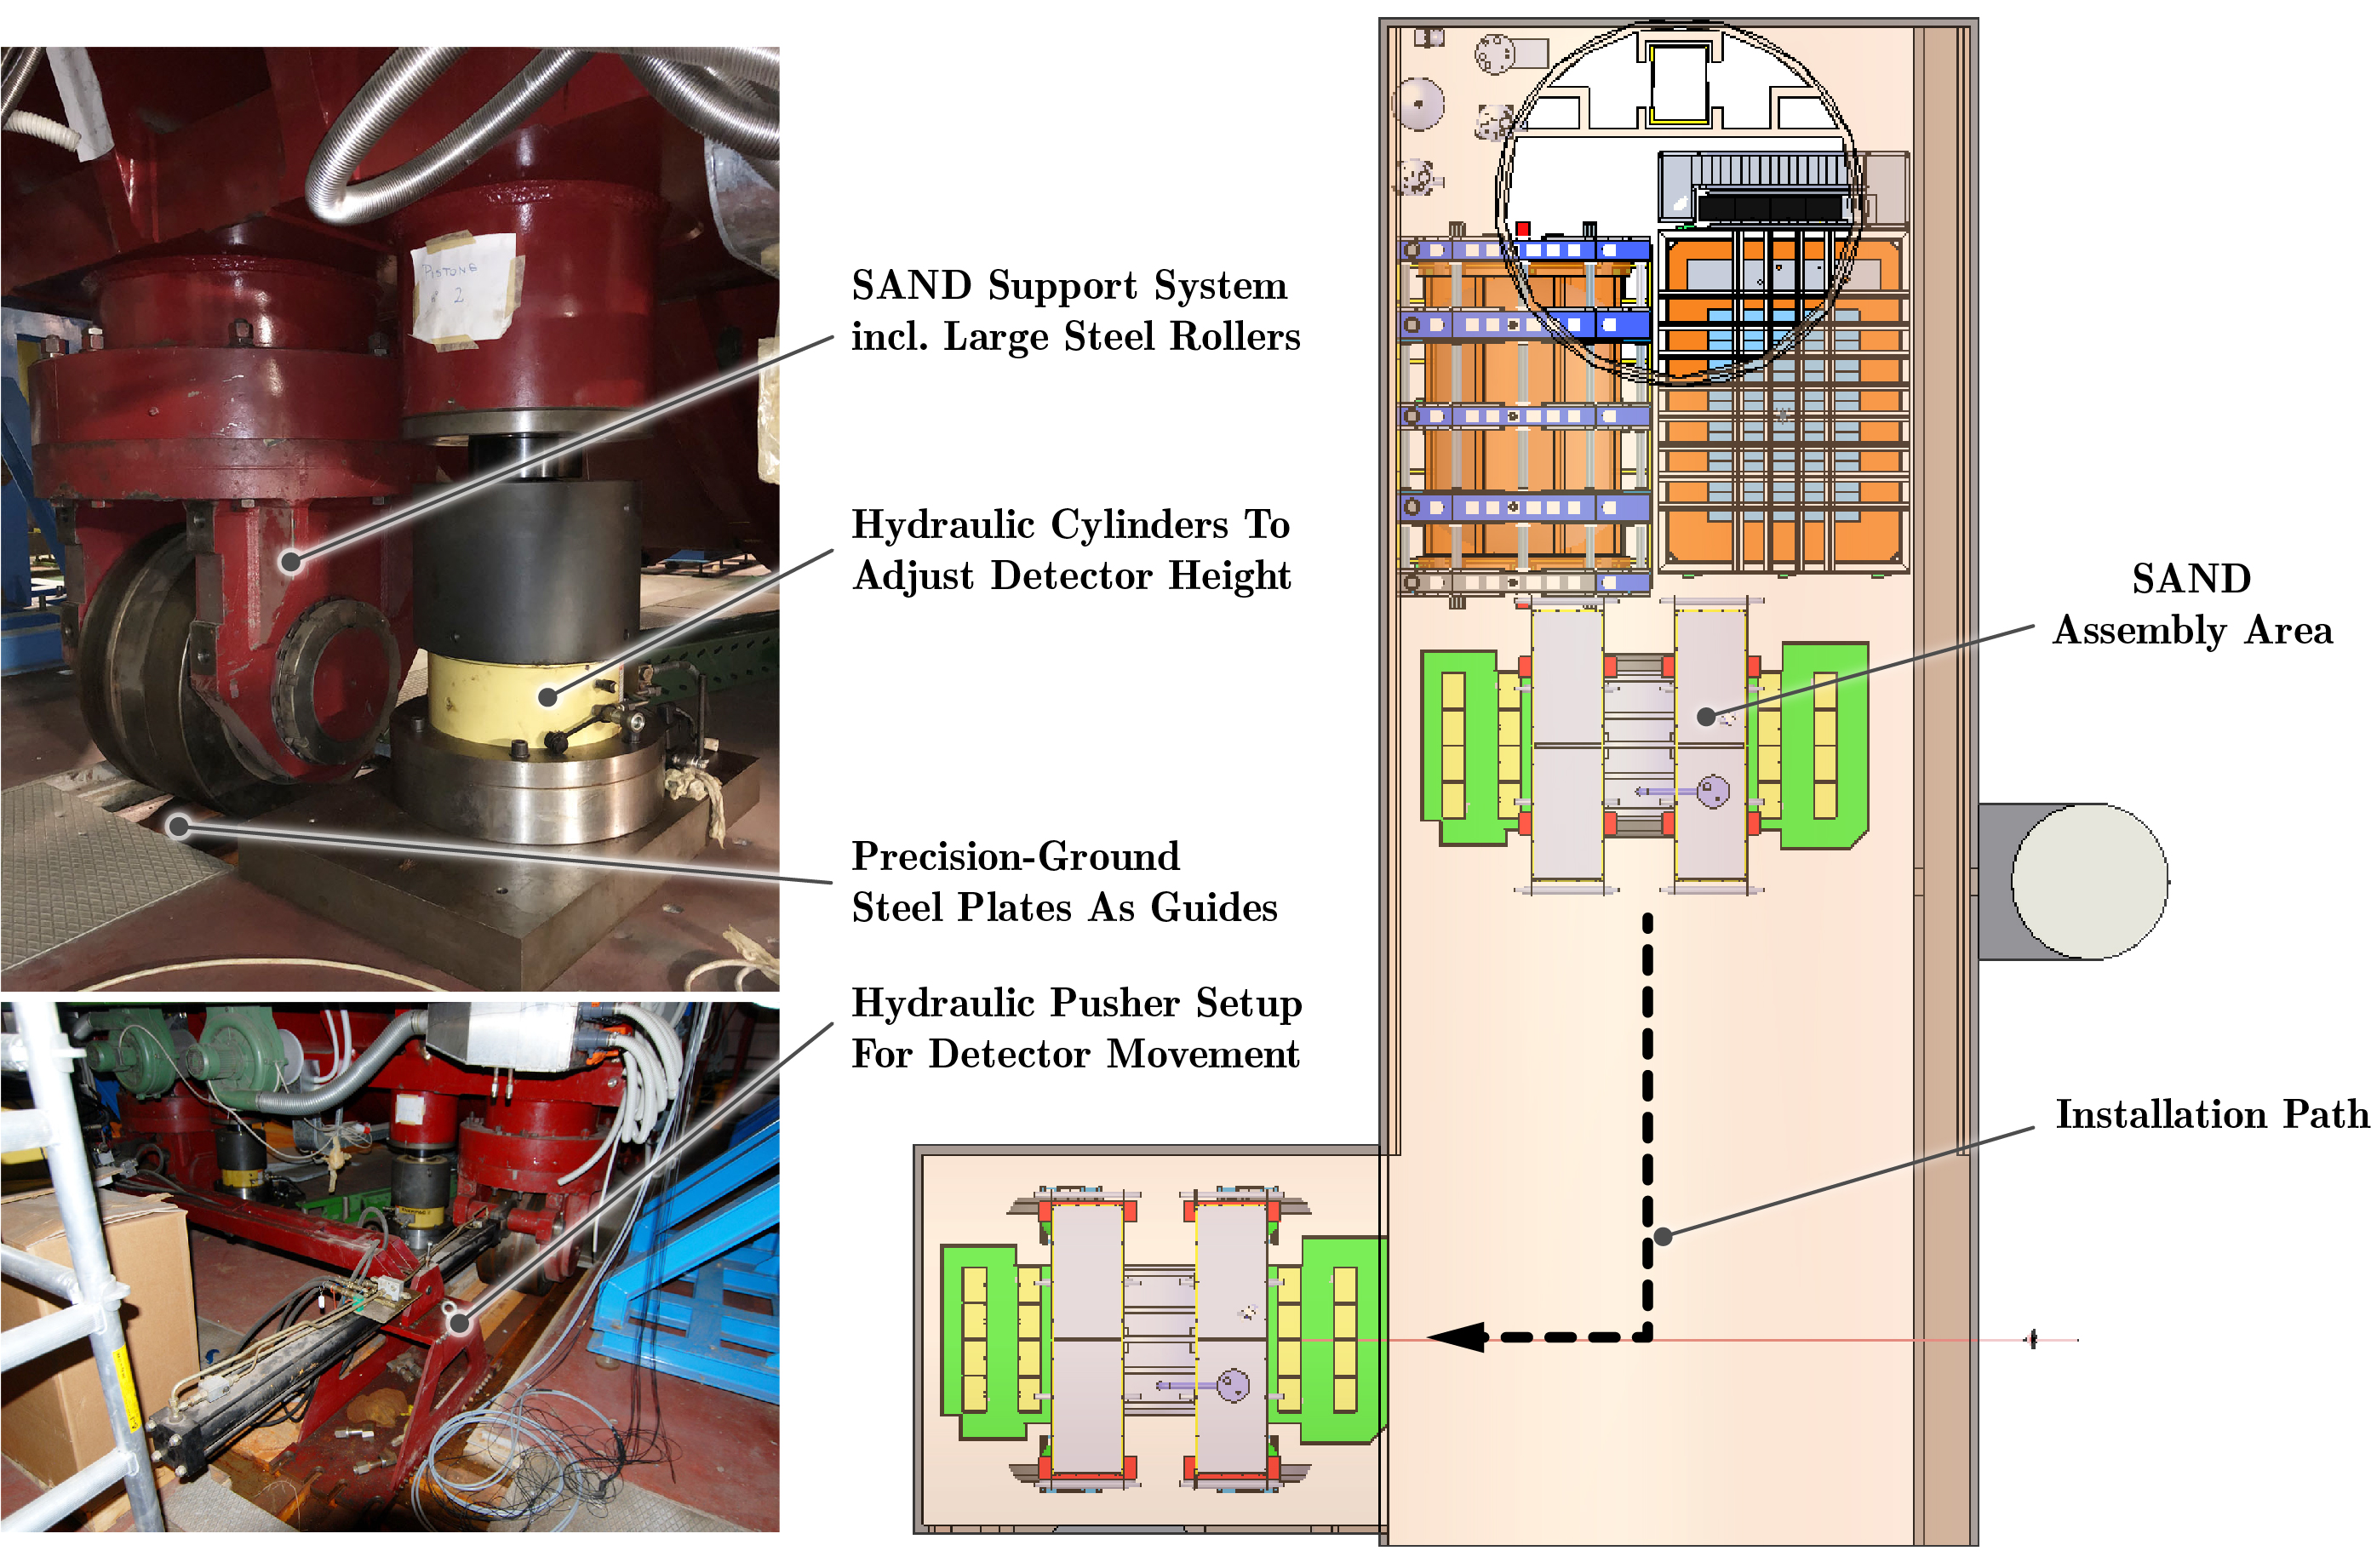
\includegraphics[width=0.8\textwidth]{graphics/i-and-i/sand_installation}
\end{dunefigure}

SAND incorporates a versatile support system with large diameter steel rollers for smooth movement and a specialized hydraulic system to adjust the detector height, see Figure~\ref{fig:sand_installation}. A hydraulic pusher system can move the detector a couple of feet per stroke along the rail system. By repeatedly moving the pusher system the beam monitor can be positioned efficiently. The steel rollers can be rotated by \SI{90}{\degree} which permits changing installation direction. This process is highlighted in Figure~\ref{fig:sand_installation} which shows the planned SAND assembly area inside the underground cavern and the installation path towards the final alcove location. In addition, alternative plans are being developed which would permit the installation and removal of SAND while the other detectors are in place. That scenario would require the assembly of the SAND electronics racks and their mezzanine structures after moving the detector close to the alcove. The SAND detector without mezzanine structures can fit in between each main detector and the cavern wall.

%%%%%%%%%%%%%%%%%%%%%%%%%%%%%%%% 
\section{PRISM Layout and Interfaces}
\label{sec:int-inst-prism-layout}

The PRISM system enables off-axis, energy-dependent neutrino beam measurements. A travel distance of \SI{30}{\m} from the nominal detector on-axis position is required to sample a wide enough energy spectrum. This requirement determines the main length of the Near Detector cavern excavation which consists of the PRISM movement range plus the ND-LAr detector width plus required conventional facility space needs on the walls. For PRISM measurements, the ND-LAr and ND-Gar move in tandem. The design also allows for individual movements that may be needed during installation and maintenance.

PRISM consists of two elements: (1) the individual detector movement platform, the motorized transport system, and rails embedded in the concrete floor; plus (2) fairly large and flexible cable carriers which support the required movement of cryogenic, power, and data lines. Figure~\ref{fig:nd_lar_setup} shows both elements for the ND-LAr subdetector.

Large and movable detectors have been built previously, primarily relying on hydraulic pushing systems (for instance, see Figure~\ref{fig:sand_installation}) which don’t permit continuous and automatic movement. Other setups incorporate rack and pinion drives which add complexity. For DUNE PRISM, an evolutionary next step incorporating  technology based on synchronized servo motor control systems will be developed. Figure~\ref{fig:prism_movement_system} highlights such a commercial (patented by Hilman Inc.), remotely operable transport system optimized for extremely heavy loads and smooth movement. It is based on a continuous track system running on a band of large-diameter, high-strength chain rollers connected to synchronized servo motors by gears and chains. Such a setup provides continuous back and forth movement without jolting.

A single transport system chain unit, as shown in Figure~\ref{fig:prism_movement_system}, can support up to \SI{200}{\metricton}. At least six to eight of such units are needed to support the >\SI{900}{\metricton} DUNE ND  detectors. Table~\ref{tab:prism_profile} summarizes a strawman PRISM movement profile and corresponding movement system requirements for an experimental off-axis run.

\begin{dunefigure}[PRISM movement system]{fig:prism_movement_system}
{Industrial transport systems for extremely heavy loads and smooth movement are commercially available. This figure shows a continuous track system running on a band of high-strength chain rollers driven by synchronized servo motors. The shown setup is patented by Hilman Inc. and would be well suited for the \dword{dune} \dword{nd} Prism movement system permitting smooth forward and back movement.}
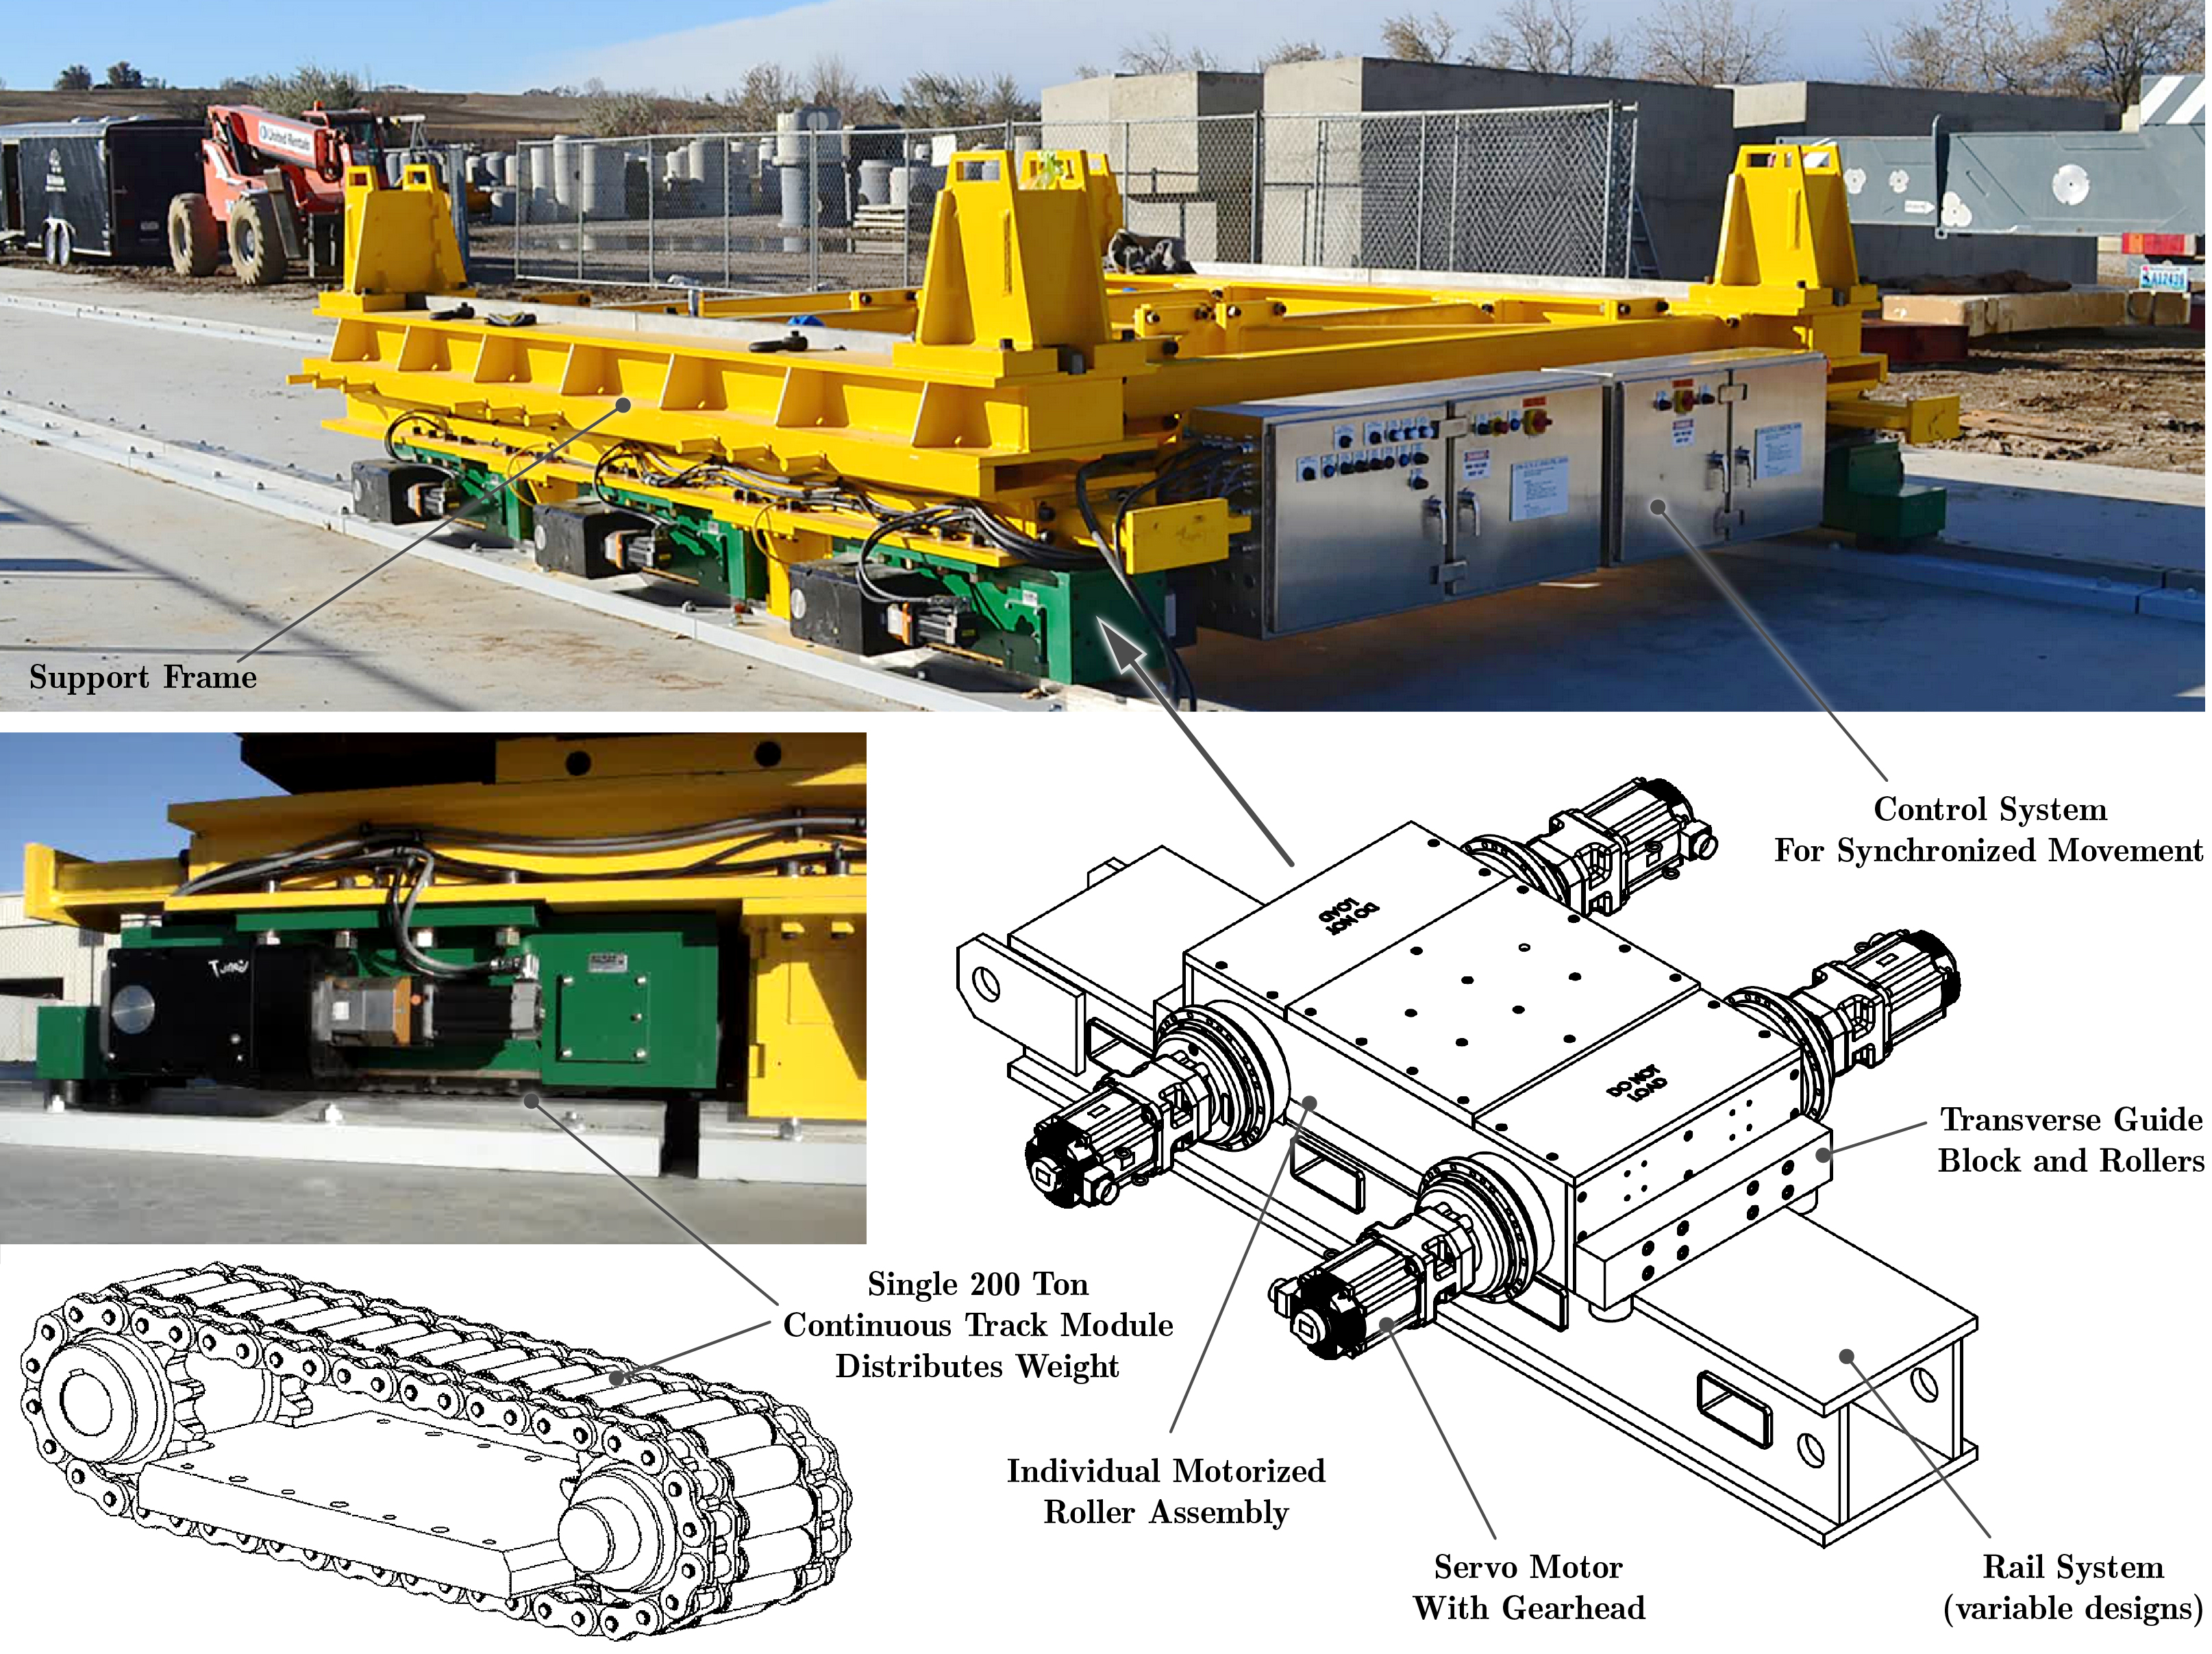
\includegraphics[width=0.8\textwidth]{graphics/i-and-i/prism_movement_system}
\end{dunefigure}

\begin{dunetable}
[Strawman PRISM movement profile]
{cc}
{tab:prism_profile}
{Strawman PRISM movement profile for an experimental off-axis run.}
Parameter & Quantity \\ \toprowrule
Travel Distance & 30.5~m \\ \colhline
Average Movement Speed & 8.5~cm/min \\ \colhline
Top Movement Speed & 10.2~cm/min \\ \colhline
Time To Reach Top Movement Speed & 60~min \\ \colhline
Resulting Linear Acceleration & 0.17~cm/sec\textsuperscript{2} \\ \colhline
Time To Travel Entire Travel Distance Without Stopping & $\sim$6~hrs \\ \colhline
Planned Stops Per Experimental Run & $\sim$9 (locations may vary per run) \\ \colhline
Stop Location - Position Repeatability & <~1~cm \\ \colhline
Stop Location - Position Measurement Accuracy & 1~mm \\ \colhline
Experimental Run Time For A Full Round Trip & 2~weeks \\ % no \colhline on final row
\end{dunetable}

\begin{dunefigure}[PRISM cable chain configuration]{fig:prism_cable_chain}
{Heavy-duty cable chains are being developed for both movable DUNE ND subdetectors. The chains carry several flexible cryogenic lines of significant outside diameter, plus electrical power and data cables.}
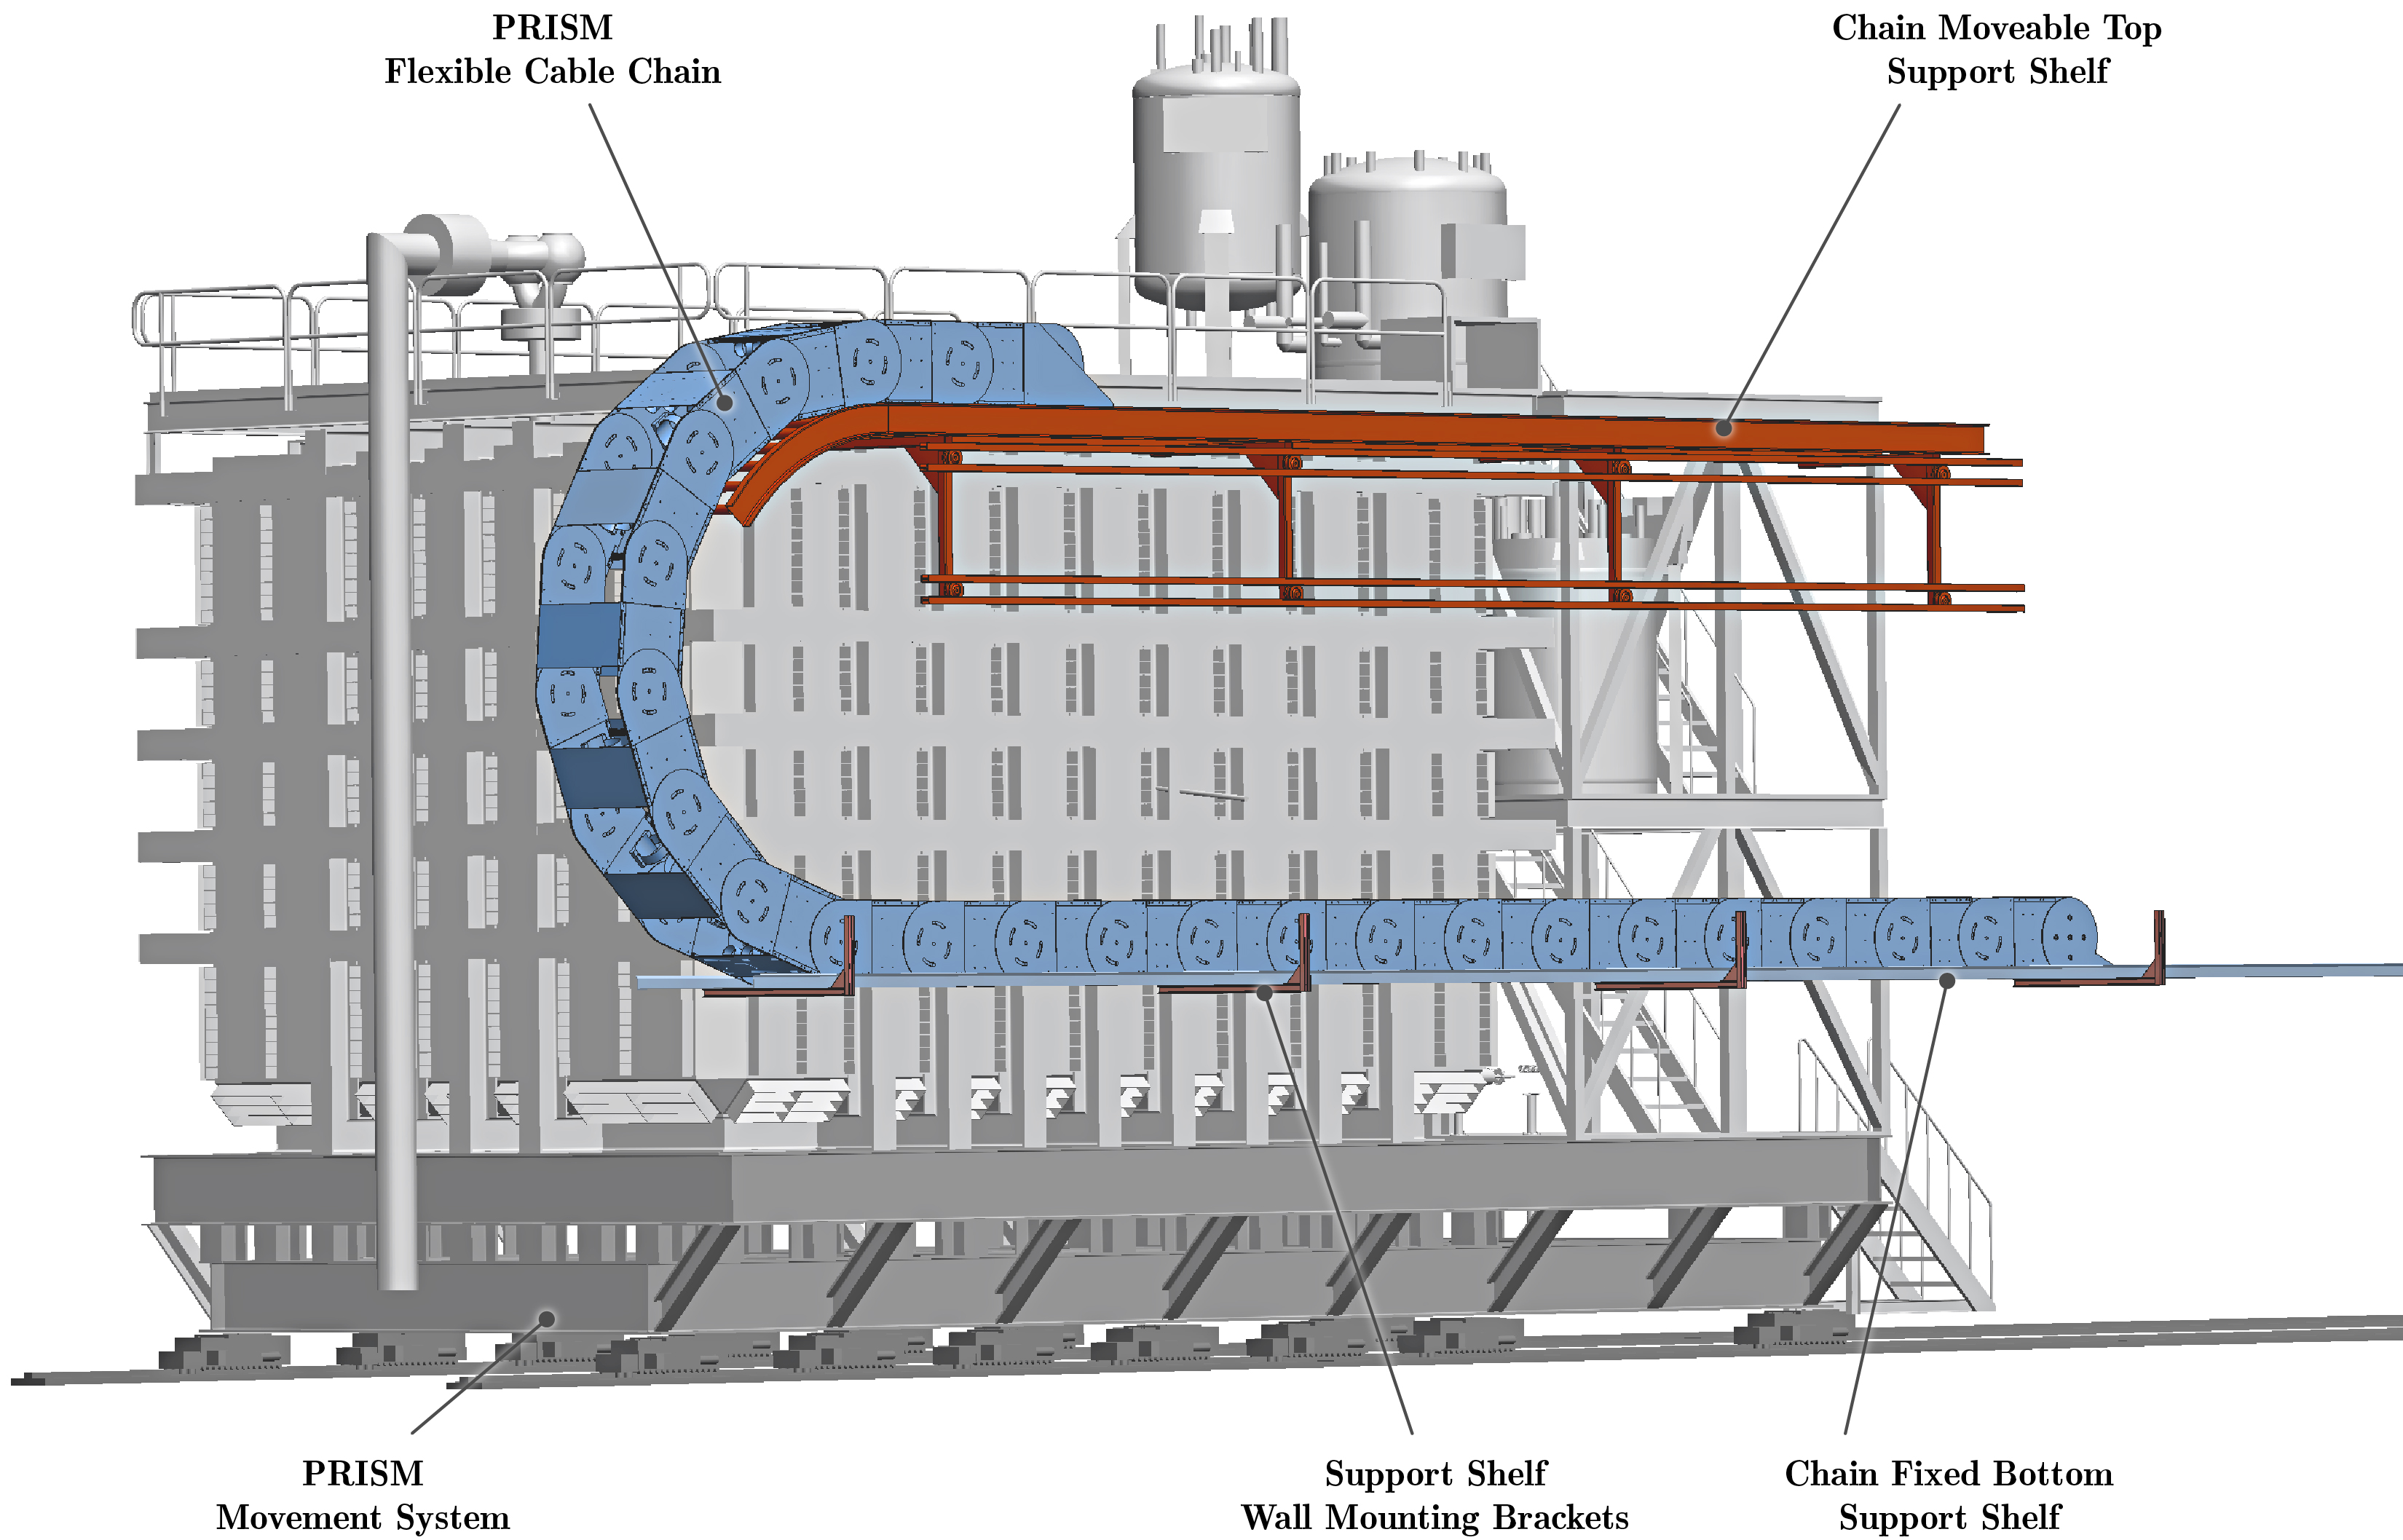
\includegraphics[width=0.8\textwidth]{graphics/i-and-i/prism_cable_chain}
\end{dunefigure}

To enable the movements of the \dword{ndlar} and \dword{ndgar} subdetectors, heavy-duty cable chains must be implemented, as  seen in Figure~\ref{fig:prism_cable_chain}. Depending on the subdetector needs, these cable chains will guide and support large and flexible cryogenic lines, electrical power as well as data cables. The cryogenic lines are made of corrugated, double-walled stainless steel pipes which are evacuated for thermal insulation.

The cable chain consists of custom-fabricated linkages made out of stamped aluminum sheets connected by low-friction bearings. Pipe holders inside the chain position and route the cryogenic lines and power cables. Due to the significant weight of the cables, the chain is not designed to be self-supporting. As shown in Figure~\ref{fig:prism_cable_chain} the bottom part of the cable chain is supported by a fixed platform, whereas the top part of the chain is carried by a moving shelf which follows at half the detector speed. The chain platform and the movable top shelf are supported from the cavern wall by conventional brackets.  The \dword{ndlar} cable chain can be seen well in the right plot of Figure~\ref{fig:nd_detector_arrangement}.

Due to the novel capabilities of the PRISM system  all core components will be prototyped, including the high-load  roller assemblies, the servo motor control system, as well as a representative length of flexible cable chain including evacuated cryogenic lines.


%%%%%%%%%%%%%%%%%%%%%%%%%%%%%%%% 
\section{Near Detector Facility Requirements}
\label{sec:int-inst-fac-req}

%%%%%%%%%%%%%%%%
\subsection{Surface Building and Rigging Access}
\label{sec:chap-id:facility:surface}

The \dword{nd} facility includes a steel-frame building located above ground on top of the primary shaft. An architectural model is shown in Figure~\ref{fig:nd_hall_3d}. Key dimensions are summarized in Table~\ref{tab:surface_building_dims}. The building is oriented parallel to the FNAL property boundary and includes architectural features to minimize impact on the neighbors. The front façade which is directed towards Wilson Hall incorporates transparent cladding which provides a well-lit highbay for equipment staging. See Figure~\ref{fig:surface_building_architectural} for a surface building architectural rendering plus floor plan.

\begin{dunefigure}[DUNE ND surface building architectural rendering]{fig:surface_building_architectural}
{The Near Detector facility includes a steel-frame building located above ground and on top of the primary shaft. The front façade incorporates transparent cladding which provides a well-lit highbay for equipment staging.}
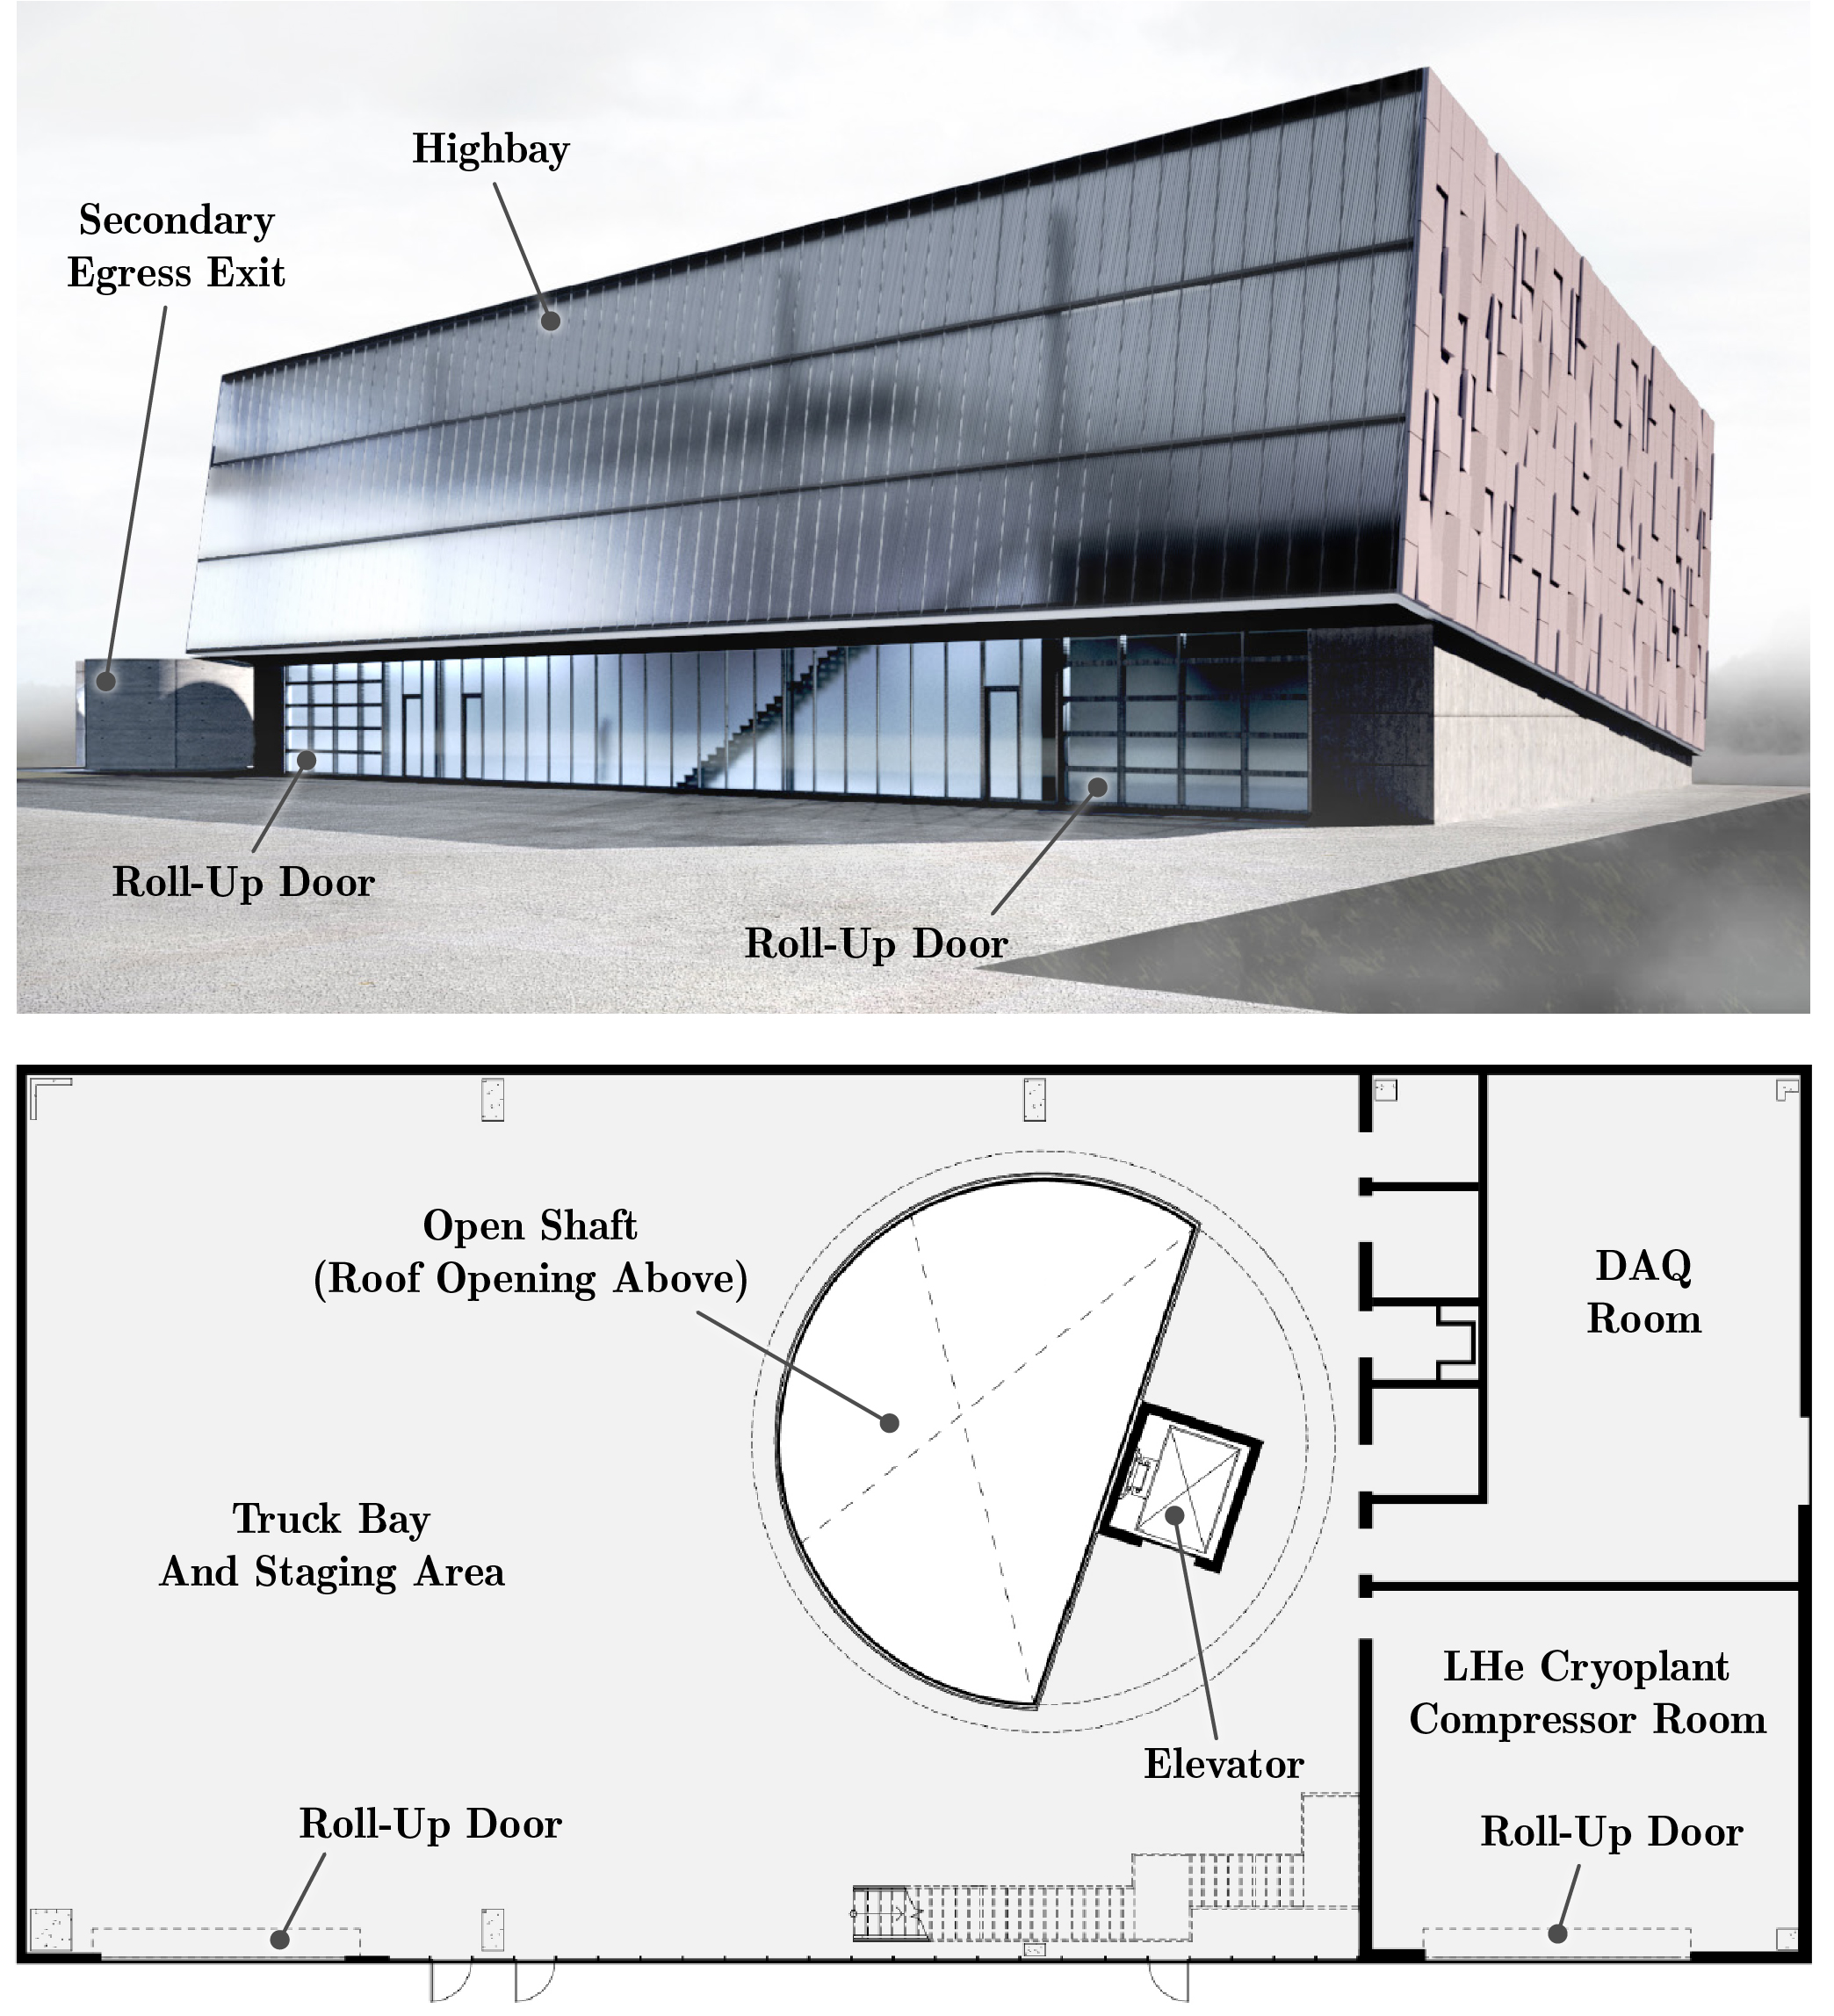
\includegraphics[width=0.7\textwidth]{graphics/i-and-i/surface_building_architectural}
\end{dunefigure}

\begin{dunetable}
[Surface building dimensions]
{cc}
{tab:surface_building_dims}
{Surface building dimensions.}
Parameter & Quantity \\ \toprowrule
Length & 128~ft \\ \colhline
Width & 64~ft \\ \colhline
Height & 38~ft \\ \colhline
Crane Capacity & 15~ton \\ \colhline
Primary Shaft Clear Diameter & 38~ft \\ % no \colhline on final row
\end{dunetable}

The surface building will house important support equipment for detector operation. As shown in Figure~\ref{fig:surface_building} a LHe cryoplant compressor room and a data acquisition (DAQ) server room will be located on the first floor. The compressor room will also accommodate a cryoplant oil purification system, an air compressor, and control racks. The DAQ room will contain a separate air conditioning unit and uninterruptible power supply.

All primary building mechanical systems will be located on the second floor, above the DAQ and compressor rooms. Most of that space will be occupied by the air handling system for the underground cavern which has to provide sufficient air flow (two redundant fan units providing 7,500~ft\textsuperscript{3}/min ventilation volume each) for oxygen deficiency hazard situations. The remaining rooms in the surface building accommodate building control systems, restrooms, storage, and fire suppression control systems.

The front side of the building will include a concrete driveway of sufficient size and strength to enable truck deliveries of detector equipment or cryogens. The LAr, LN, and GHe storage tanks will be located in the vicinity, see Figure~\ref{fig:surface_building}. The surface building highbay will permit the loading and unloading of standard tractor trailers. The highbay rollup door is dimensioned to allow backing in of a tractor trailer loaded with fully assembled LAr modules.

\begin{dunefigure}[Detailed surface building layout]{fig:surface_building}
{The surface building houses important support equipment for detector as well as building operation. In addition, the building provides rigging and staging capabilities to lower equipment into the underground cavern.}
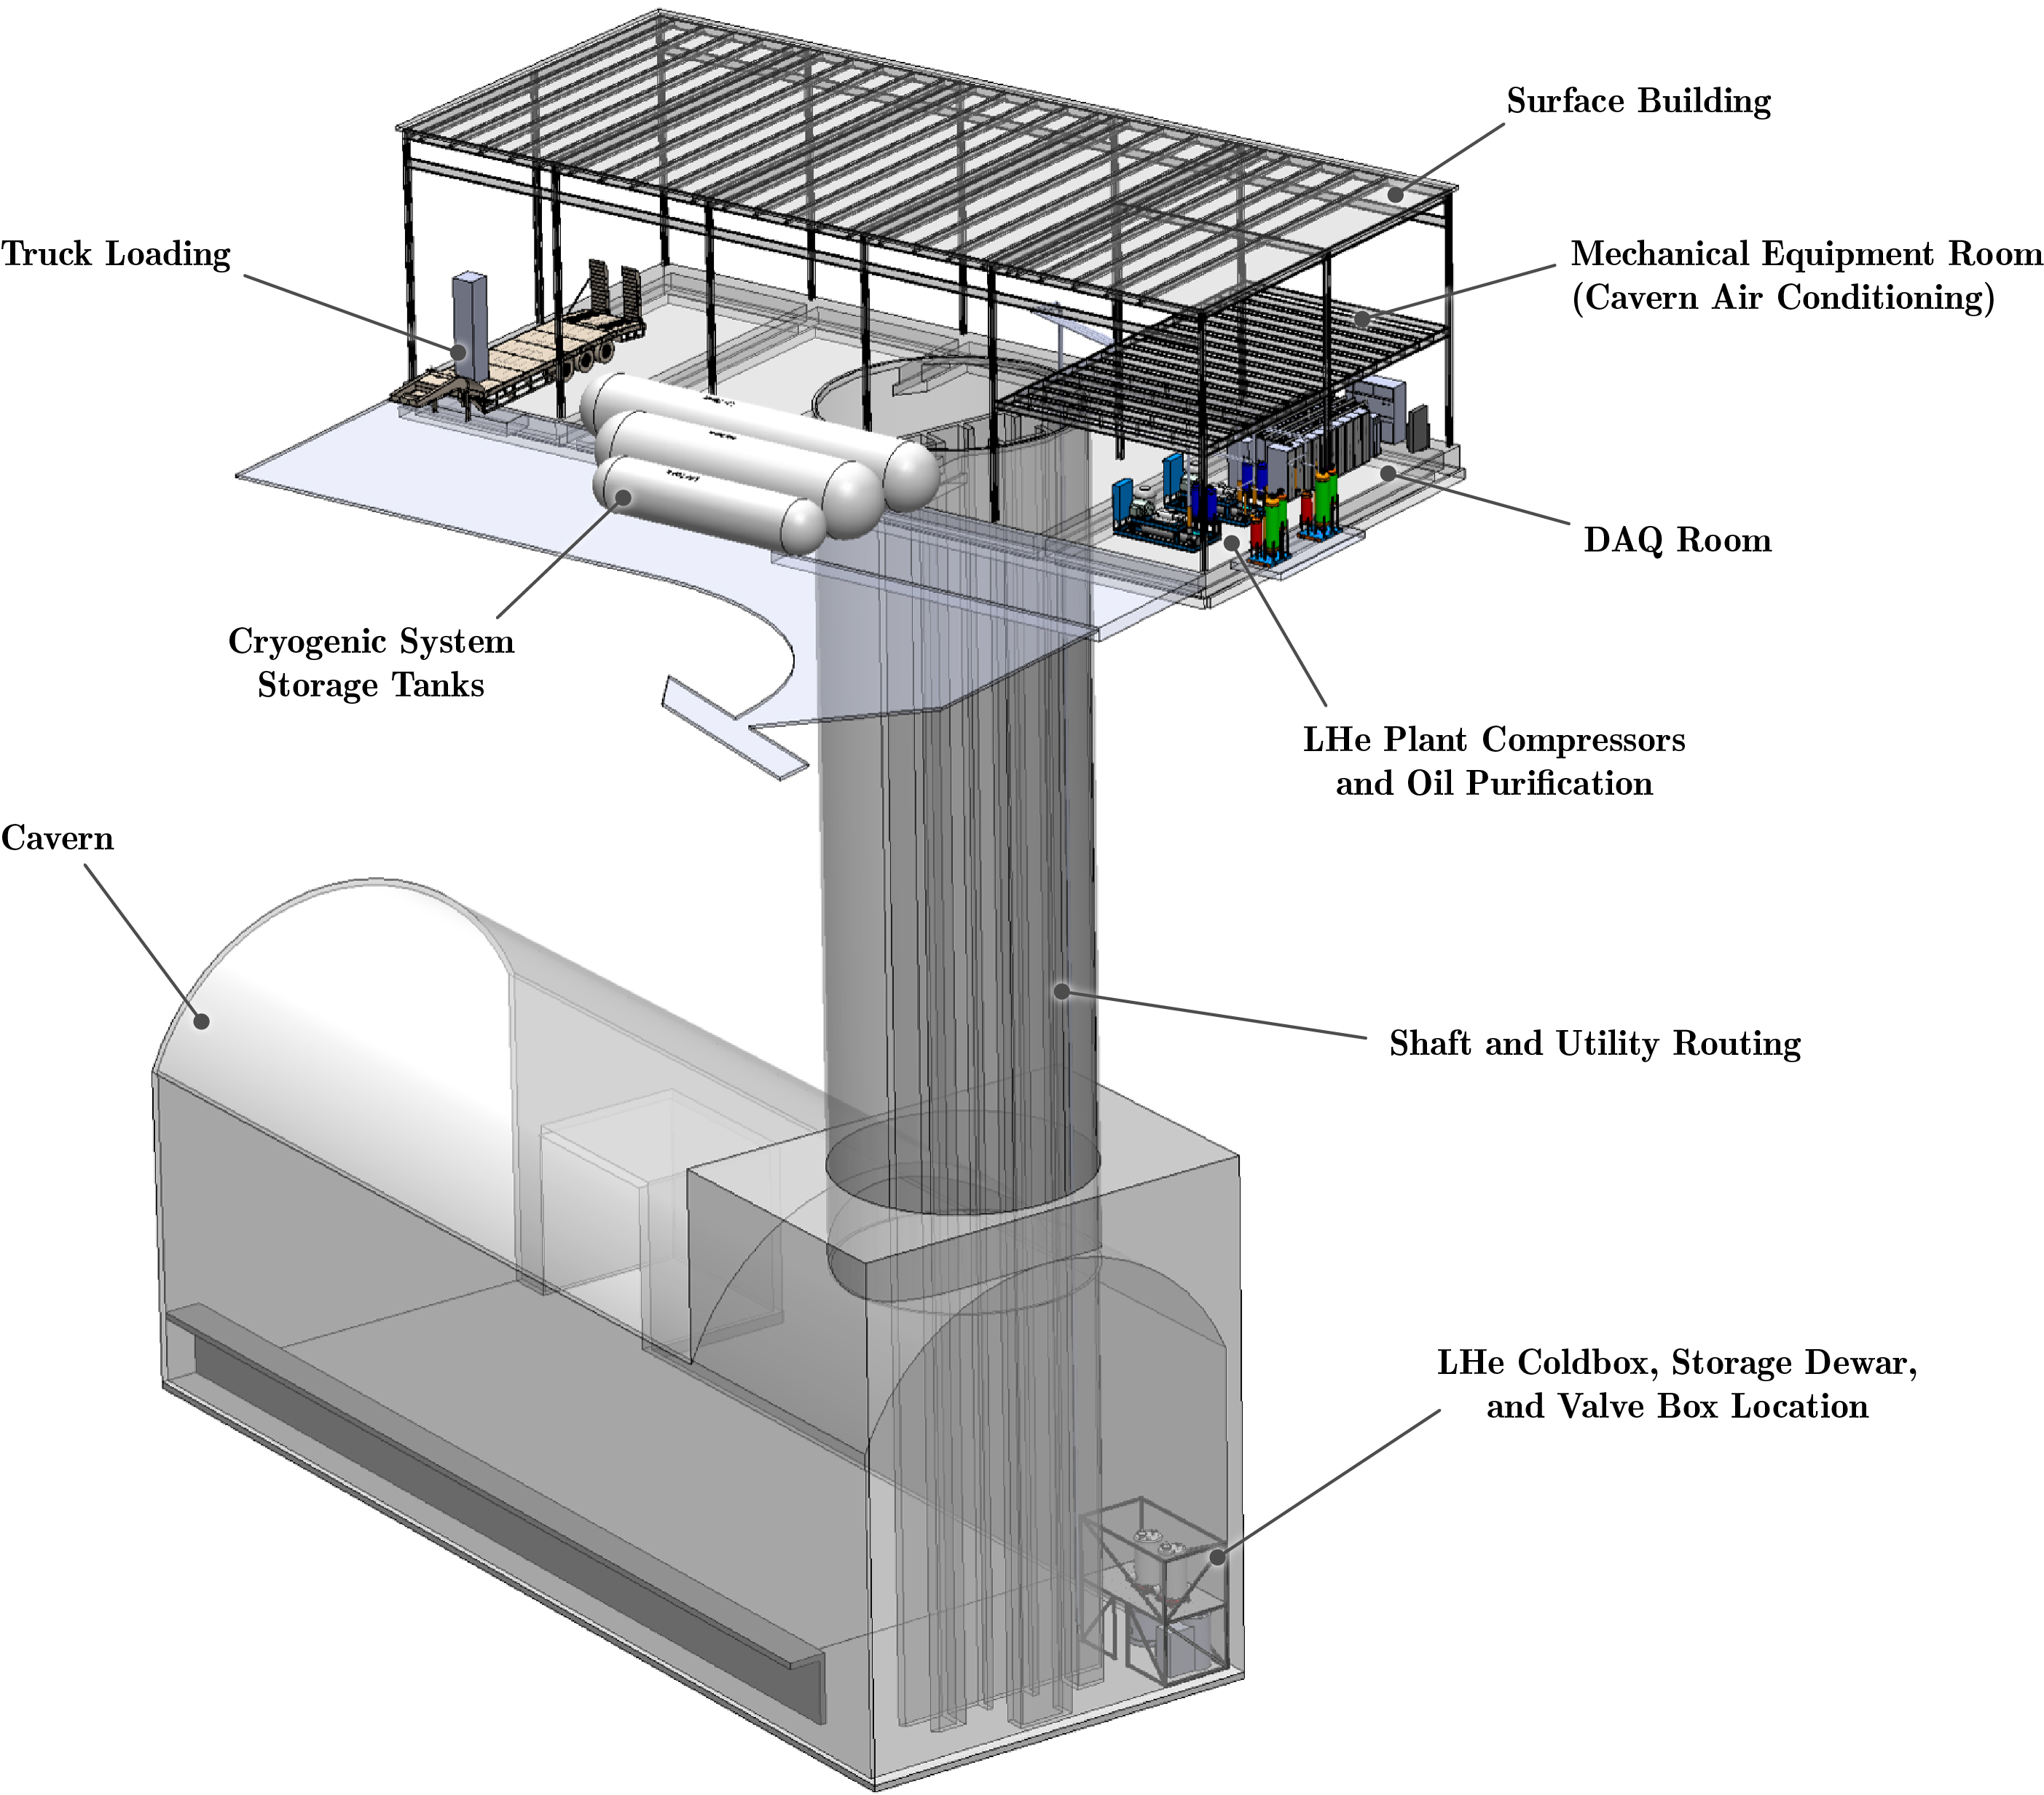
\includegraphics[width=0.7\textwidth]{graphics/i-and-i/surface_building}
\end{dunefigure}

The open shaft to the underground cavern provides detector rigging access. A significant portion of the shaft is also reserved for a personnel elevator and the large ventilation ducts. Electrical power and cryogenic distribution lines will also be routed through the shaft. Since the highbay has only limited building height and crane capacity, a large roof hatch located above the shaft will be utilized to lower heavy detector components underground. Figure~\ref{fig:surface_building_shaft_access} illustrates a few representative rigging setups utilizing rental cranes which can be positioned outside the surface building. The primary shaft diameter has been chosen to fit the ND-GAr pressure vessel and the SAND solenoid cryostat. Neither detector can be disassembled into smaller pieces or rotated. The large shaft size would also permit rigging fully welded and assembled ND-LAr cryostat warm structure panels underground which could significantly ease underground installation. 

\begin{dunefigure}[DUNE ND rigging access]{fig:surface_building_shaft_access}
{A roof hatch in the surface building and above the shaft will be utilized to lower large and heavy detector components underground utilizing rental cranes. The primary shaft diameter is large enough for the ND-GAr pressure vessel or the SAND solenoid cryostat. Such a shaft size would permit rigging fully welded ND-LAr cryostat warm structure panels underground which could significantly ease underground installation.}
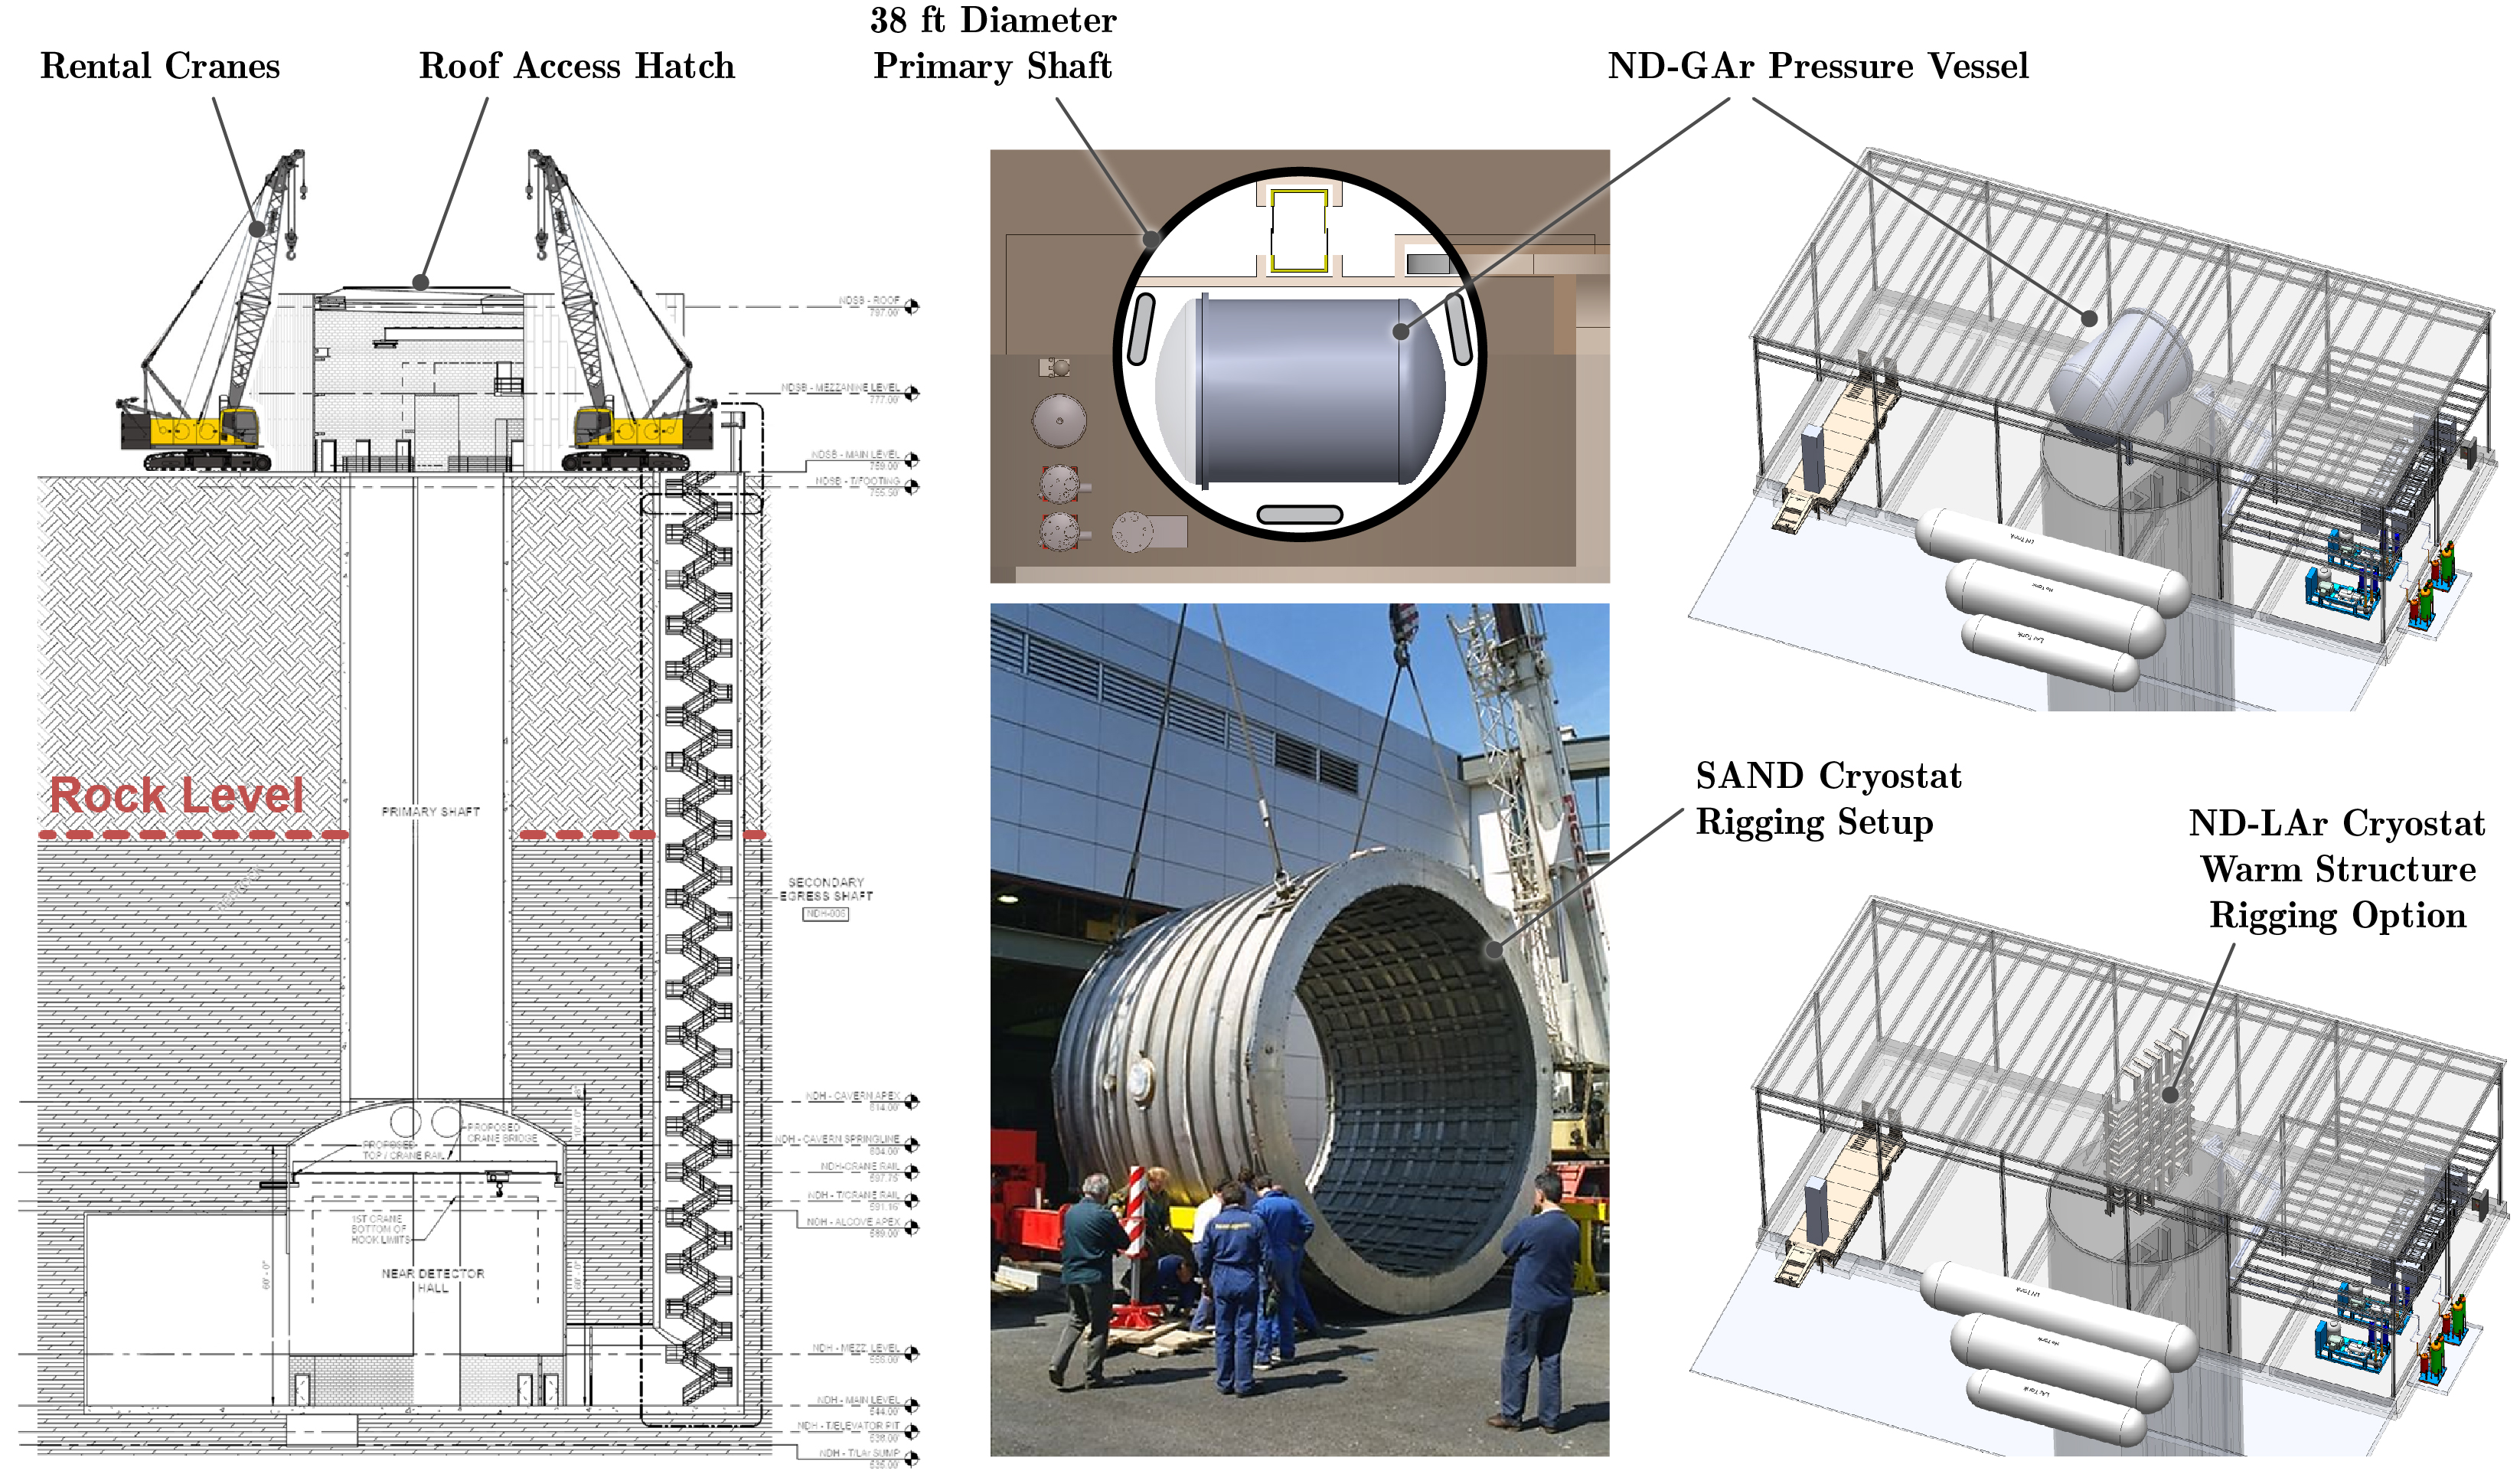
\includegraphics[width=0.9\textwidth]{graphics/i-and-i/surface_building_shaft_access}
\end{dunefigure}

%%%%%%%%%%%%%%%%
\subsection{Auxiliary Building Systems}
\label{sec:chap-id:facility:additional}

%ODH, Electrical, Electrical Power, Crane, Climate, Fire Safety

A new electrical main power feed will be installed to service the Near Detector Facility. A preliminary estimate for detector power requirements is shown in Table~\ref{tab:power_needs}. A corresponding power distribution line diagram for the Near Detector scientific equipment has been developed, see Figure~\ref{fig:power_distribution}. Conventional Facilities will design and install the main circuit breaker panels and the conventional power transformers in the surface building as well as the cavern. All three subdetectors will be electrically isolated from building ground to reduce electrical noise and cross-talk. Therefore, the Near Detector Integration \& Installation electrical engineering group will design the respective subdetector isolation transformers and cable routing. A detailed grounding plan for each subdetector will be developed during the preliminary design phase. The ND-LAr subdetector will closely follow ProtoDUNE design approaches and lessons learned. The SAND subdetector is a self-contained detector with an isolated ground.

\begin{dunetable}
[Near Detector electrical power needs]
{cc}
{tab:power_needs}
{Near Detector Electrical Power Needs.}
System & Power \\ \toprowrule
LHe Cryoplant (surface building) & 500~kVA \\ \colhline
DAQ Room and UPS (surface building) & 75~kVA \\ \colhline
ND-LAr & 225~kVA \\ \colhline
ND-GAr & 225~kVA \\ \colhline
SAND & 500~kVA \\ \colhline
LHe Cold Box & 75~kVA \\ \colhline
PRISM Motors & 75~kVA \\ \colhline
LAr Cryogenics & 45~kVA \\ % no \colhline on final row
\end{dunetable}

\begin{dunefigure}[DUNE ND power distribution diagram]{fig:power_distribution}
{DUNE ND detector power distribution diagram.}
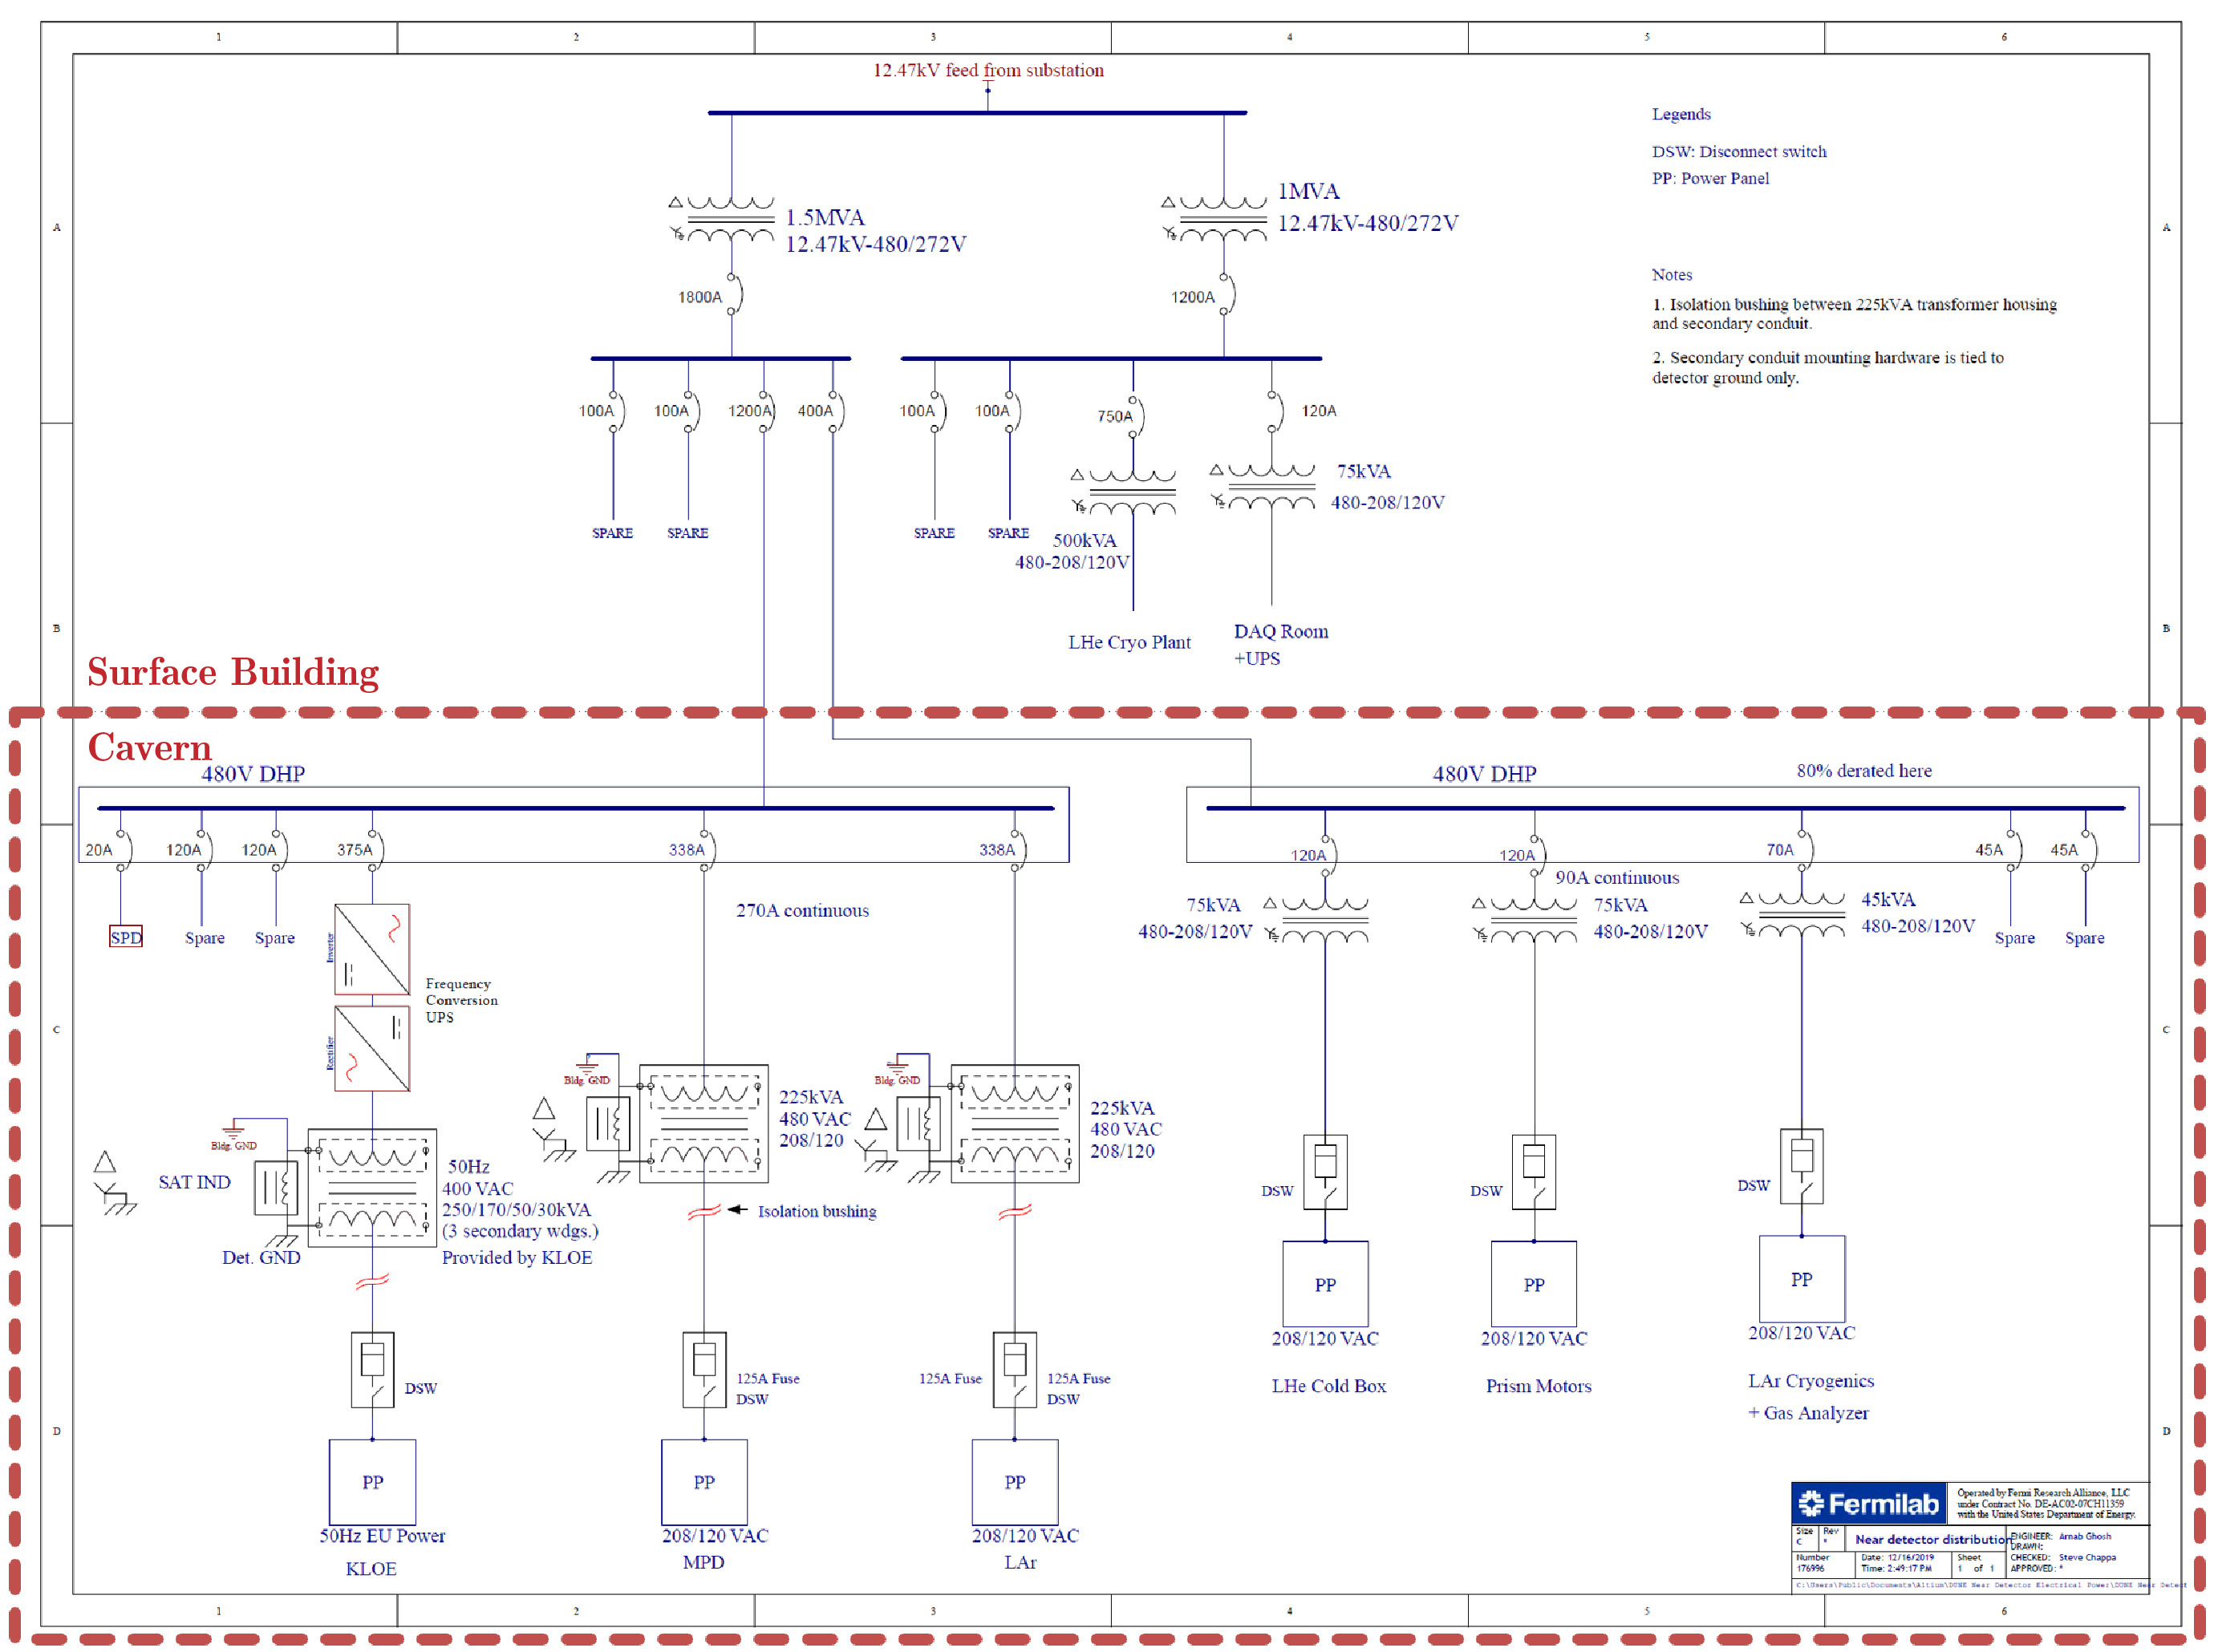
\includegraphics[width=1.0\textwidth]{graphics/i-and-i/power_distribution}
\end{dunefigure}

The SAND subdetector is built based on European electricity standards. Therefore, the US power feed frequency must be converted from 60 to 50~Hz. As shown in Figure~\ref{fig:power_distribution}, a commercially available frequency conversion system similar to ones used in UPS units can be installed. This approach would be an elegant and efficient way of adapting the subdetector to the US line frequency and eliminating the need of modifying SAND components.

Additional building services will be required in addition to electrical power. These include:
\begin{itemize}[noitemsep,topsep=-10pt]
\item Air conditioning,
\item Industrial water cooling,
\item Compressed air,
\item Lighting,
\item Stand-by power,
\item Access control,
\item Fire safety systems, and
\item Oxygen deficiency hazard safety systems.
\end{itemize}
Requirements for most of these systems are comparable to similar detector facilities and will be fully defined during the conventional facilities final design phase. More unique design features for these systems are described next.

The Near Detector cavern temperature should be controlled to \SI{21}{\celsius} $\pm$ \SI{5}{\celsius}. To limit condensation on cryogenic lines and the cryostat structures cavern humidity should ideally be maintained below 50$\%$~RH at \SI{21}{\celsius}. However, such an air conditioning system could become quite expensive since water may be continually present inside the cavern. A proposed, more cost-effective air conditioning approach would be to generate conditioned (dried) air at the surface building and blow it into the cavern. This approach can control temperature and would significantly reduce cavern humidity. However, such an approach cannot actively control or guarantee cavern humidity which will depend on the water present in the cavern or weather conditions on the surface. Localized heating or air flow may be required to minimize excessive ice forming on cryogenic systems or to reduce water formation on electronics and could be implemented after initial detector operational experiences.

\begin{dunefigure}[ODH Ventilation Duct Routing]{fig:odh_vents}
{Routing of the ODH ventilation ducts (the supply line is in green and the exhaust line is in dark pink) inside the Near Detector cavern. Only the LAr detector is shown for clarity. The exhaust line must be directed to the bottom of the cavern to be able to collect argon gas along the travel path of the ND-LAr detector. The large ventilation ducts will be routed through the main shaft to the surface building mechanical equipment room (see Figure~\ref{fig:surface_building}).}
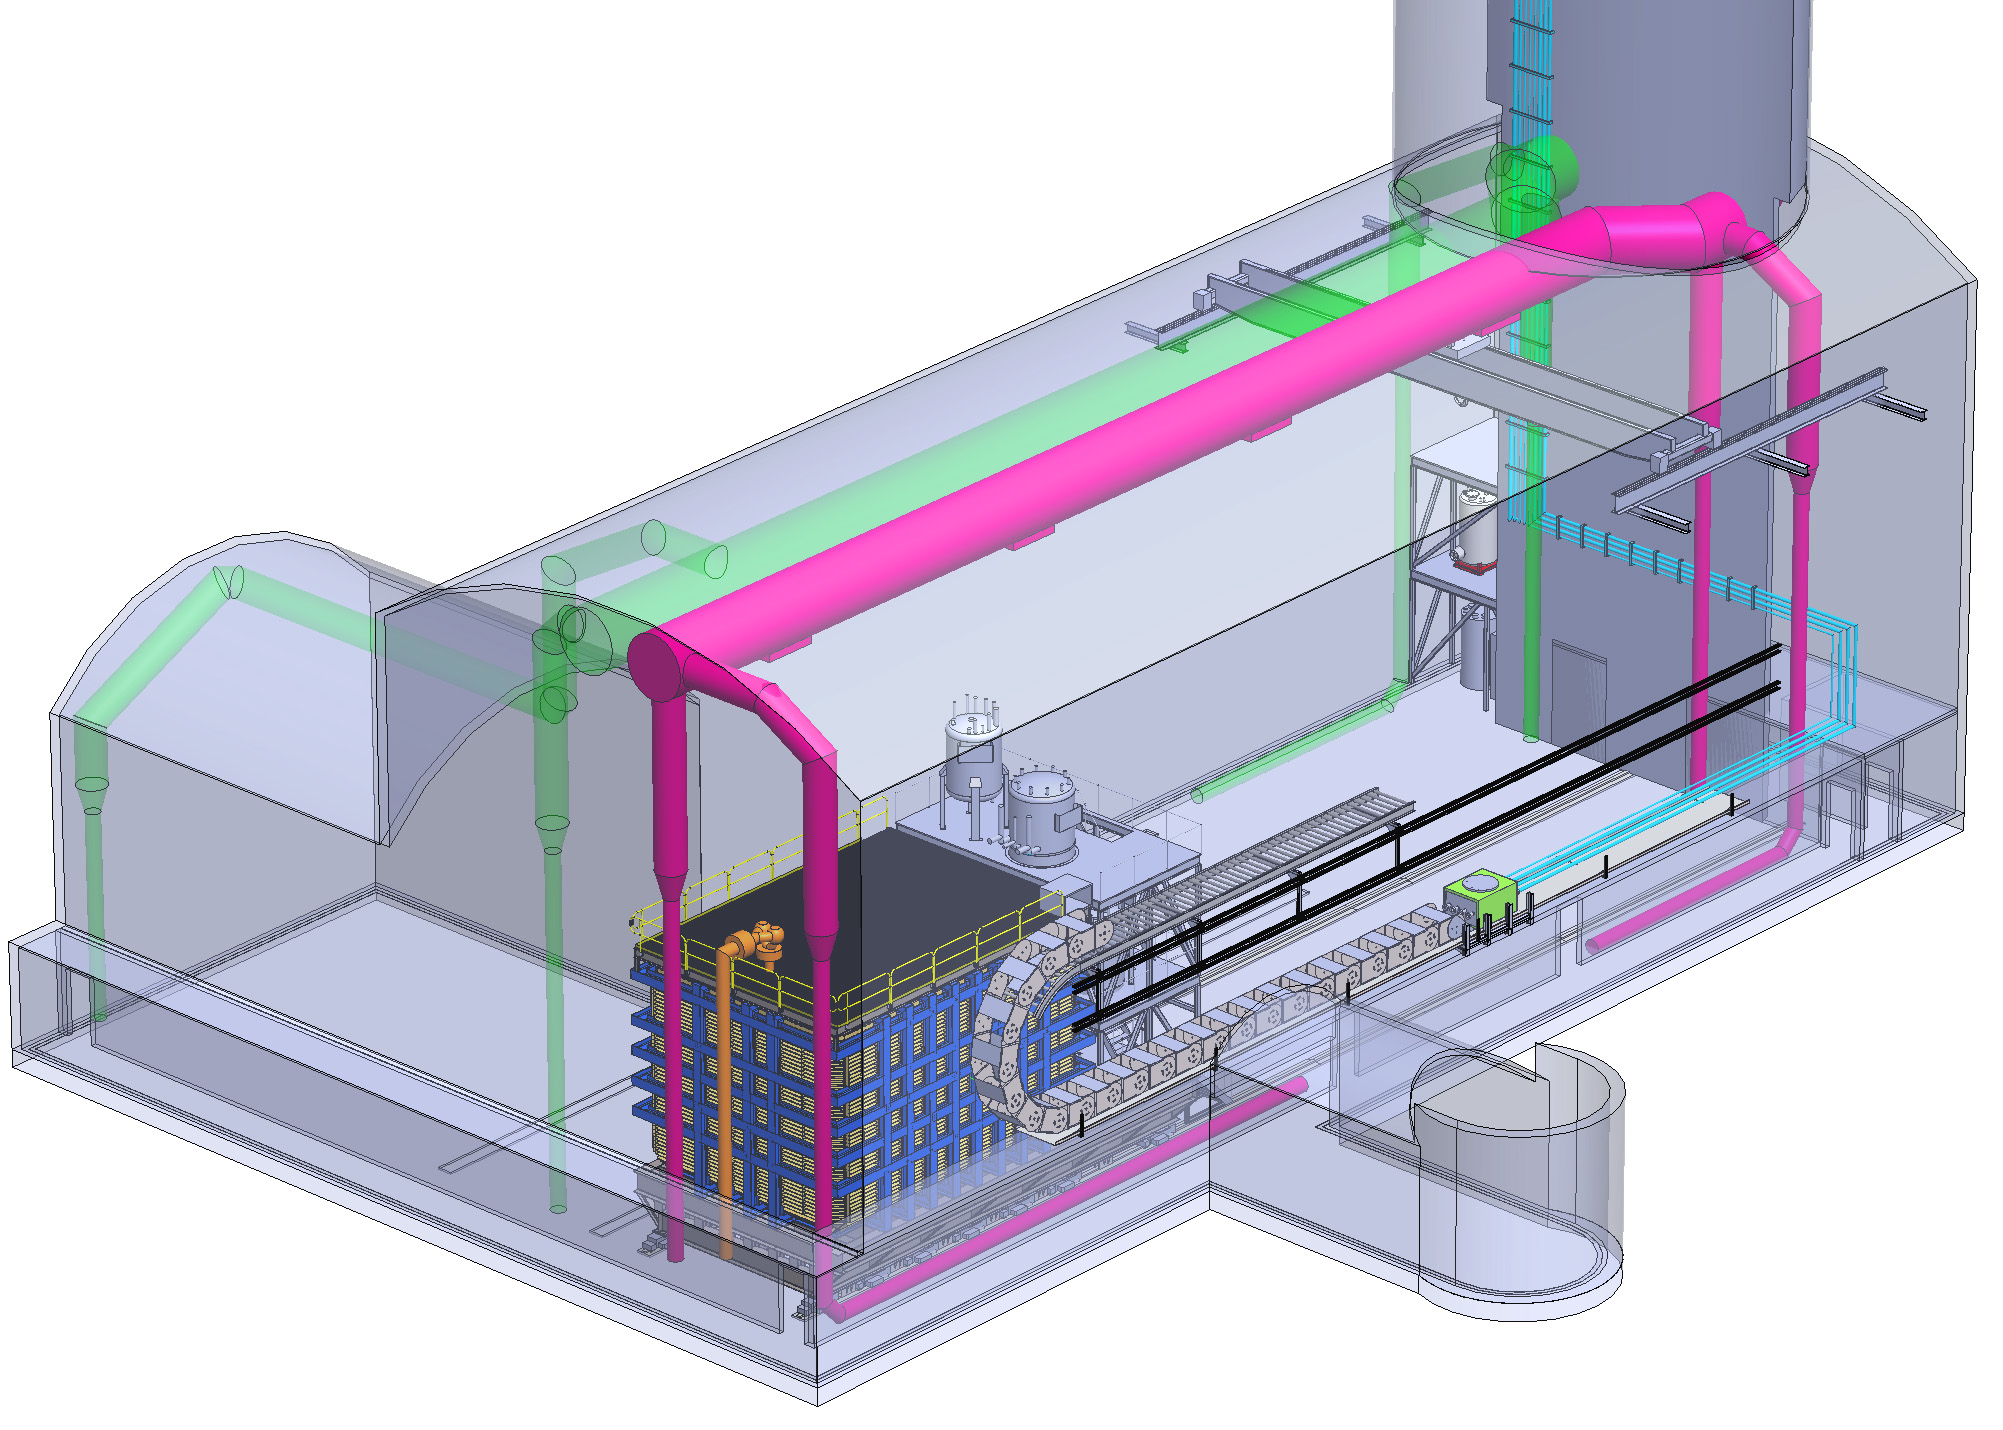
\includegraphics[width=0.7\textwidth]{graphics/i-and-i/odh_vents}
\end{dunefigure}

An ODH scoping calculation has been performed for the Near Detector cavern. Based on this study the air ducts will be  initially designed to provide >7,500~ft\textsuperscript{3}/min ventilation volume. Two fan units will be implemented to provide redundancy. Since large quantities of liquid helium (lighter than air) as well as liquid argon (heavier than air) cryogens are present in the cavern the ventilation ducts will have adjustable louvers on the top as well as the bottom of the cavern. A suggested routing of the ventilation ducts is shown in Figure~\ref{fig:odh_vents}. Similar to ProtoDUNE the current ND-LAr detector design incorporates a cryostat emergency vent discharging to the bottom of the cavern floor in close vicinity to the ODH ventilation ducts. The cavern is expected to be designated class ODH-1. Such a hazard class would require the use of personal oxygen monitors and self-rescue oxygen packs. A detailed safety analysis according to the FNAL ES\&H manual will be performed once the subdetector designs have further matured.

Industrial water cooling will be required in the underground cavern for the LHe coldbox as well as detector power supplies and electronics. Compressed air will be needed for underground cryogenic valve operation. These systems plus standby power and lighting needs will be specified during the detector preliminary design phase. DUNE systems engineering as well as DUNE Integration \& Installation maintain integrated CAD models for clash detection between detectors and conventional facilities equipment.



%%%%%%%%%%%%%%%%%%%%%%%%%%%%%%%% 
\section{Overall Installation Sequence and Schedule}
\label{sec:int-inst-seq-sched}

\fixme{We may want to use a standardized schedule format. (Anne)}

An initial installation schedule, see Figure~\ref{fig:installation_schedule}, has been developed based on the available design information for the cavern and the detectors (see previous sub-sections). Individual detector installations must be staggered in time due to movement constraints given by the size of the equipment and the limited space available underground. For instance, SAND should be moved in place before the other two detector installations can be finalized. The ND-LAr membrane cryostat requires final assembly and welding in situ. ND-GAr installation can only be initiated once the ND-LAr membrane cryostat has been completed.

\begin{dunefigure}[DUNE Near Detector Facility Installation Schedule]{fig:installation_schedule}
{Proposed \dword{dune} \dword{nd} Facility installation schedule. Installation will commence ("FY~x+1" in the displayed schedule) once cavern construction has been completed and authorization to use the \dword{nd} facility has been granted. Assembly of the full \dword{dune} \dword{nd} reference design including checkout and transition to operation will require approximately three years to complete.}
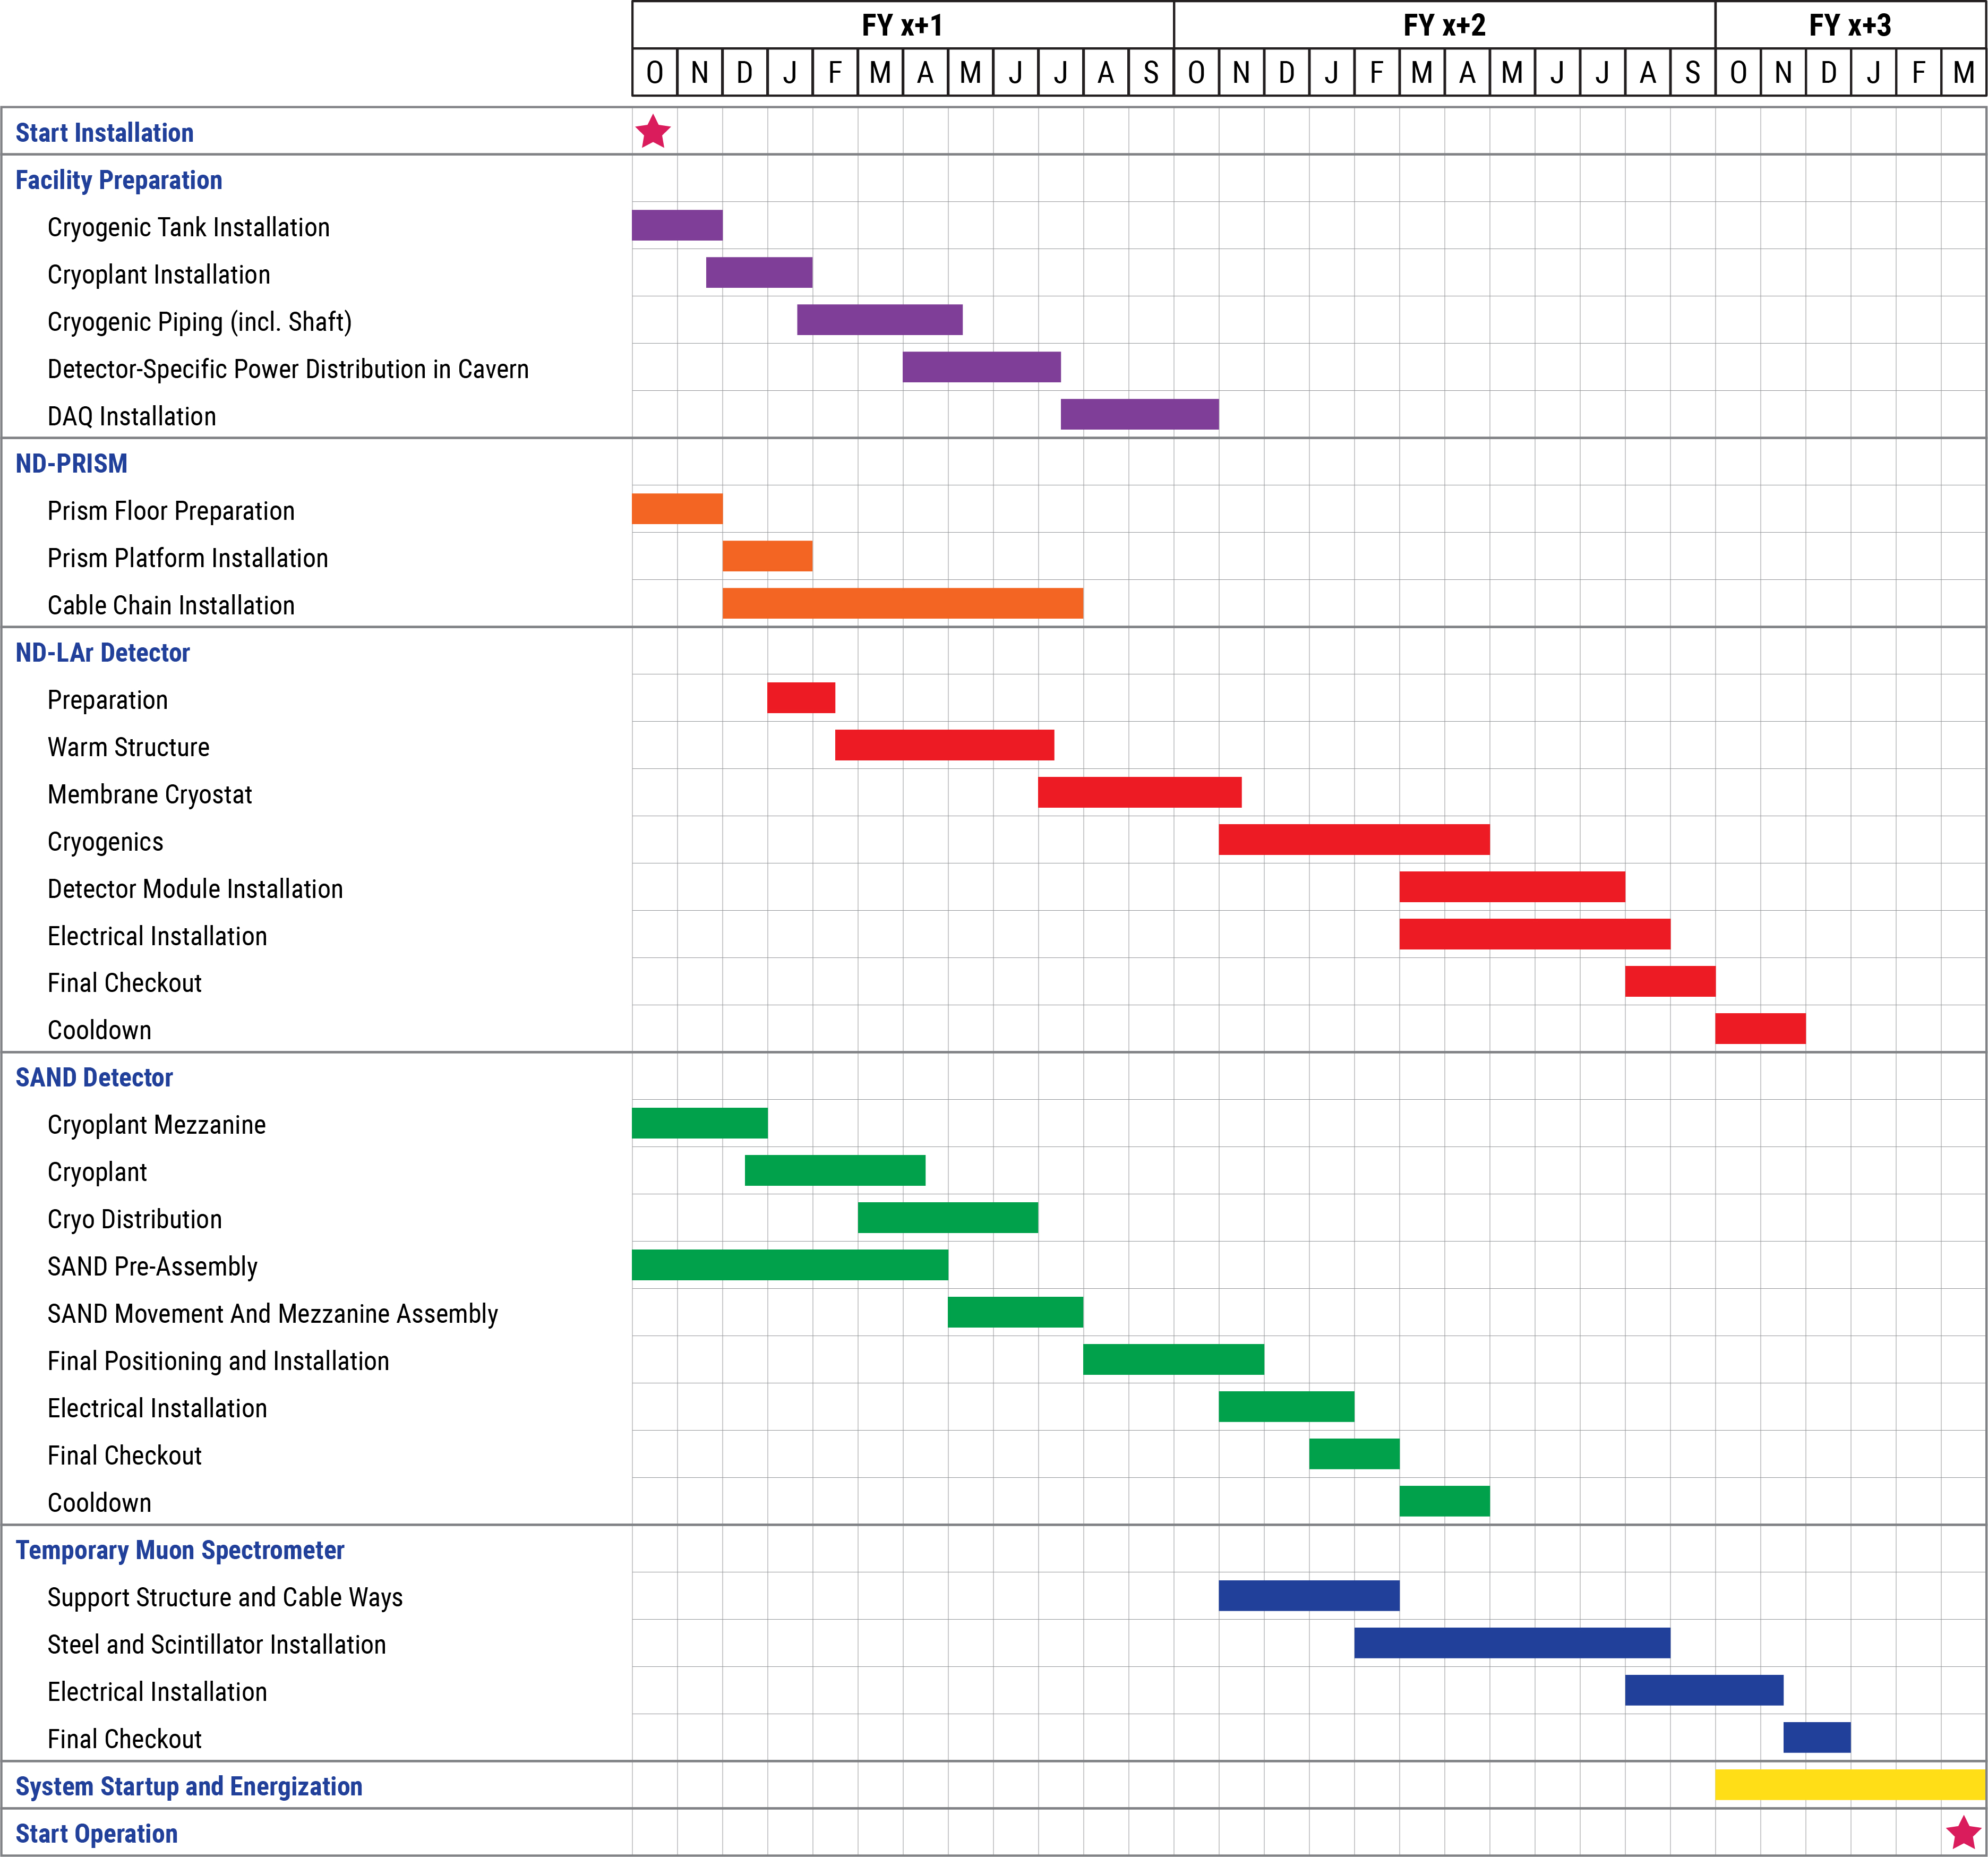
\includegraphics[width=1.0\textwidth]{graphics/i-and-i/installation_schedule}
\end{dunefigure}

Installation activities will commence once cavern construction has been completed and authorization to use the Near Detector facility has been granted. Assembly of the full DUNE Near Detector reference design including checkout and transition to operation will require approximately 3 years to complete. Near Detector installation will require close coordination between the detector consortia and the DUNE project. All on-site installation activities will be coordinated and scheduled by a DUNE~ND Integration \& Installation group to ensure safe occupancy of the installation areas and to optimize manpower utilization. In addition, the DUNE~ND Installation group will provide common rigging hardware, clean room structures, lifting platforms, and shared tooling and fixturing to perform typical installation tasks. To support the detector consortia during detector assembly, \dword{dune} \dword{nd} Integration \& Installation will employ a core group of four mechanical technicians, shift supervisors, an electrical technician and engineer, and two manufacturing engineers. At the same time, the individual detector consortia will provide additional personnel and specialized tooling needed to ensure that the three-year installation schedule can be achieved. This approach will require in-depth agreements between DUNE and the detector consortia. These agreements together with a detailed installation workflow will be developed during the final design phase once all detector component designs have matured.

Figure~\ref{fig:installation_schedule} outlines a potential sequence of Near Detector installation activities. Once authorization to use the building structures has been granted essential detector infrastructure will be installed first. This work includes the installation of cryogenic tanks and cryoplant equipment in the surface building. Likewise, the ND-GAr and SAND LHe coldbox equipment and mezzanine structure (located underground, see Figure~\ref{fig:sand_cryo_location} and Figure~\ref{fig:surface_building}) plus the PRISM rail system and moving platforms will be installed during this first phase.

Next, major rigging activities will be initiated. SAND components will be lowered into the cavern to permit assembly of the main structural components including the coil cryostat. Assembly will occur underground in the vicinity of the shaft. Once the SAND cryostat has been inserted into the iron yoke and the yoke end plates have been installed the detector can be moved close to the beam monitor alcove. All subsequent SAND assembly steps will take place in this location which frees up space close to the shaft to complete parallel assembly of the ND-LAr detector warm structure and to initiate the installation of the membrane cryostat. The SAND cryogenic distribution line installation will be completed during that later time frame. All major rigging activities will require the rental and installation of gantry crane structures with sufficient (>50~ton) load capacity. The current LBNF preliminary cavern design only includes a 15~ton overhead crane which is not sufficient for any of the detector assembly steps.

The installation of the ND-LAr cryostat follows a process similar to ProtoDUNE. Once the PRISM movement frame has been installed the platform surface will be shimmed to bring it within the membrane cryostat flatness requirements. Next, the conventional, warm cryostat structure will be erected and the inner steel membrane welded leak tight. At this point the membrane cryostat company can proceed with assembling the insulating foam structure, the inner stainless-steel liner, and the bottom LAr valve feedthrough. A temporary top plate cover will be mounted to enable leak-checking of the full cryostat assembly.

An extended period of cryogenic installation activities follows the completion of the ND-LAr cryostat assembly. A prefabricated, large mezzanine structure will be erected to support the ND-LAr purification system, and all the cryogenic equipment and piping will be installed. That work also includes connecting the cryostat to the cable chain (see Figure~\ref{fig:prism_cable_chain}) which has been mounted to the cavern wall earlier.

Individual ND-LAr pixelated detector modules, which will be pre-assembled and tested at FNAL in a separate production facility (IREC, currently under construction), will be transported into the Near Detector surface building and assembled to a large flange combining an entire detector row (see Figure~\ref{fig:nd_lar_details}). These rows will be lowered into the cavern and immediately installed in the cryostat. Installation of all electrical utilities, racks, and control chassis will occur in parallel.

Once SAND has been moved into its final position and the ND-LAr membrane cryostat has been assembled the cavern space under the vicinity of the shaft becomes available for ND-GAr detector assembly. Major parts of the ND-GAr detector are still in an early design stage. Therefore, the proposed schedule is based on a preliminary detector configuration as described in sub-section \ref{sec:chap-id:details:mpd}.

The ND-GAr detector magnet structure consists of five individual cryostats which will be lowered into the cavern in a pre-assembled state. Subsequently, these cryostats must be mounted on the PRISM support platform and connected to each other underground. Similarly, the TPC and its pressure tank will be pre-assembled above ground and lowered into the cavern as one unit. A special lifting fixture will permit the insertion of the tank into the magnet structure. Added time is allocated for effort to complete the complex assembly and installation of the TPC components underground. Cryogenic equipment installation and connections to the cryostat can proceed in parallel. Next, the ND-GAr electromagnetic calorimeter segments plus any additional tracking devices will be installed in between the cryostat structures and around the detector ends. At this point assembly of the main ND-GAr detector components will be complete and final detector and electrical integration can start followed by several months of checkout and magnet cooldown.

Finally, individual detector start-up can commence which is a multi-step process requiring subsystem sign-offs, safety approvals, and step-wise equipment energization. During that time frame coordination of and responsibility for Near Detector installation activities will gradually transition to the international detector consortia and their scientific operation teams. At this point, the DUNE Near Detector Facility is ready to start scientific operation.


\begin{comment}
\fixme{ML: These sections still need to be incorporated.}

%%%%%%%%%%%%%%%%% from Tim?
\subsection{Standard: SAND First}
\label{sec:int-inst-seq-std}

%%%%%%%%%%%%%%%%% 
\subsection{Backup: SAND Later}
\label{sec:int-inst-seq-bkup}



%%%%%%%%%%%%%%%%%%%%%%%%%%%%%%%%
\section{Interfaces}
\label{sec:int-inst-interface}

\fixme{We may use individual interface tables in the above sections? Anne}
Table~\ref{tbl:int-inst-interfaces} contains a summary and brief description of all the interfaces between the integration and installation consortium and other consortia, working groups, and task forces, with references to the current version of the interface documents describing those interfaces.  
Drawings of the mechanical interfaces and diagrams of the electrical interfaces are 
included in the interface documents as appropriate.
It is expected that further refinements of the interface documents will take place prior to the final \dword{prr} for the detector. The interface documents specify the responsibility of different consortia or groups during all phases of the experiment including design and prototyping, integration,  installation, and  commissioning.


\begin{dunetable}
[Integration and installation interface links]
{p{0.25\textwidth}p{0.5\textwidth}l}
{tbl:int-inst-interfaces}
{Integration and installation interface links}
Interfacing System & Description & Linked Reference \\ \toprowrule
\dword{ndlar}      &  (desc)
& \citedocdb{?} \\ \colhline

\dshort{duneprism} &  (desc)
& \citedocdb{?} \\ \colhline

\dshort{tms}  &  (desc)
& \citedocdb{?} \\ \colhline

and so on     &  (desc)
& \citedocdb{?} \\
\end{dunetable}

%%%%%%%%%%%%%%%%%%%%%%%%%%%%%%%%
\section{Risks and Mitigations}
\label{sec:int-inst-risks}

\fixme{ (This section will also cover delayed detector arrival)}
Table~\ref{tab:risks:int-inst} contains a list of all the
risks that \dword{dune} is currently holding in the I\&I risk register.  Each line includes the official \dword{dune} risk register identification number, a description of the risk, the proposed mitigation for the risk, and finally three columns rating the post-mitigation (P)robability that the risk described comes to pass, the degree of (C)ost risk for that line, and the degree of (S)chedule risk.  Risk levels are defined as (L)ow (<10\% probability of occurring, <5\% cost impact, <2 month schedule impact), (M)edium (10 to 25\% probability of occurring, 5\% to 20\% cost impact, 2 to 6 month schedule impact), or (H)igh (>25\% probability of occurring, >20\% cost impact, >6 month schedule impact).  Most of these risks are reduced to a ``Low'' level following mitigation (as shown in the table), although several of them currently hold a higher risk levels (pre-mitigation), due to the early stage of development of the \dword{ndlar} system relative to other systems.  

In the following sections, we present a narrative description of each of the risks and the proposed mitigation.

\fixme{Anne needs to get risk table template put together}
%\input{generated/risks-longtable-ND-LAr.tex}

\begin{dunetable}
[Placeholder for risks table]
{cc}
{tab:risks:int-inst}
{Placeholder for Risks Table - it will be generated from a spreadsheet}
Rows & Counts \\ \toprowrule
Row 1 & First \\ \colhline
Row 2 & Second \\ \colhline
Row 3 & Third \\ % no \colhline on final row
\end{dunetable}

%%%%%%%%%%%%%%%%%%%%%%%%%%%%%%%% 
\section{Schedule}
\label{sec:int-inst-org-sched}

Table \ref{tab:int-inst-sched} lists key milestones in the design, validation, construction, and installation of the near detector.  These milestones include external milestones indicating linkages to the main \dword{dune} schedule (highlighted in color in the table), as well as internal milestones such as design validation and technical reviews.

\fixme{Anne to get list of main DUNE sched items from Eric J before making the real table template}
\begin{longtable}
{p{0.75\textwidth}p{0.25\textwidth}}
\caption{\dshort{ndlar} consortium schedule}\\ \colhline
\rowcolor{dunetablecolor}Milestone & Date   \\ \toprowrule


\rowcolor{dunepeach}Beneficial occupancy of cavern 1 and \dword{cuc}& \cucbenocc      \\ \colhline
Initial batch (80 PD modules) assembled  & March 2023\\ \colhline

\rowcolor{dunepeach}Top of \dword{detmodule} \#1 cryostat accessible& \accesstopfirstcryo      \\ \colhline
Third batch (320 PD modules) arrive at US PD Reception Facility  & January 2024\\ 

\label{tab:int-inst-sched}
\end{longtable}


%%%%%%%%%%%%%%%%%%%%%%%%%%%%%%%% 
\section{Prototyping Plans}
\label{sec:int-inst-proto}


%\begin{comment}
\fixme{The following sections are not in the new structure; I'm keeping them at the end here for now, in case you want to include one or more of them later.}
%%%%%%%%%%%%%%%%%%%%%%%%%%%%%%%% Not in Tim's new organization
\section{Safety Concerns}
\label{sec:int-inst-safety}

%%%%%%%%%%%%%%%%%%%%%%%%%%%%%%%% Not in Tim's new organization
\section{Quality Assurance}
\label{sec:int-inst-qa}

%%%%%%%%%%%%%%%%%%%%%%%%%%%%%%%% Not in Tim's new organization
\section{Transport and Handling}
\label{sec:int-inst-transport}


%%%%%%%%%%%%%%% Not in Tim's new organization
\subsection{Participating Institutions}
\label{sec:fdsp-org-inst}

The \dword{ndlar} consortium benefits from the contributions of many institutions and facilities in \fixme{several countries? or the U.S. and ??}.  Table~\ref{tab:int-inst-institutes}
lists the member institutions. 

\begin{longtable}
{ll}
\caption{\dshort{ndlar} consortium institutions}\\ \colhline
\rowcolor{dunetablecolor} Member Institute  &  Country       \\  \toprowrule
univ 1 &  \\ \colhline
univ 2 &  \\ \colhline
univ 3 &  \\ 
\label{tab:int-inst-institutes}
\end{longtable}

\end{comment}







